%%%%%%%%%%%%%%%%%%%%%%%%%%%%%%%%%%%%%%%%%%%%%%%%%%%%%%%%%%%%%%%%%%%%%%%%%%%%%%%%%%%%%%%%
%%%%%%%%%%%%%%%%%%%%%%%%%%%%%%%%%%%%%%%%%%%%%%%%%%%%%%%%%%%%%%%%%%%%%%%%%%%%%%%%%%%%%%%%
%%                                                                                    %%
%%               MASTER THESIS - SEBASTIANO MENEGHIN - 2024 - KTH                     %%
%%                                                                                    %%
%%%%%%%%%%%%%%%%%%%%%%%%%%%%%%%%%%%%%%%%%%%%%%%%%%%%%%%%%%%%%%%%%%%%%%%%%%%%%%%%%%%%%%%%
%%%%%%%%%%%%%%%%%%%%%%%%%%%%%%%%%%%%%%%%%%%%%%%%%%%%%%%%%%%%%%%%%%%%%%%%%%%%%%%%%%%%%%%%
%%
%%%%%%%%%%%%%%%%%%%%%%%%%%%%%%%%%%%%%%%%%%%%%%%%%%%%%%%%%%%%%%%%%%%%%%%%%%%%%%%%%%%%%%%%
%%                                PREAMBLE
%%%%%%%%%%%%%%%%%%%%%%%%%%%%%%%%%%%%%%%%%%%%%%%%%%%%%%%%%%%%%%%%%%%%%%%%%%%%%%%%%%%%%%%%
%%
%% INFORMATION ON THIS PREAMBLE:
%%
%% forked from https://gits-15.sys.kth.se/giampi/kthlatex kthlatex-0.2rc4 on 2020-02-13
%% expanded upon by Gerald Q. Maguire Jr.
%% This template has been adapted by Anders Sjögren to the University
%% Engineering Program in Computer Science at KTH ICT. This adaptation was to
%% translation of English headings into Swedish as the addition of Swedish.
%% Many thanks to others who have provided constructive input regarding the template.

%% Make it possible to conditionally depend on the TeX engine used
\RequirePackage{ifxetex}
\RequirePackage{ifluatex}
\newif\ifxeorlua
\ifxetex\xeorluatrue\fi
\ifluatex\xeorluatrue\fi

\ifxeorlua
%% The following is to ensure that the PDF uses a recent version rather than the typical PDF 1-5
%% This same version of PDF should be set as an option for hyperef

\RequirePackage{expl3}
\ExplSyntaxOn
%pdf_version_gset:n{2.0}
%\pdf_version_gset:n{1.5}

%% Alternatively, if you have a LaTeX newer than June 2022, you can use the following. However, then you have to remove the pdfversion from hyperef. It also breaks hyperxmp. So perhaps it is too early to try using it!
%\DocumentMetadata
%{
%% testphase = phase-I, % tagging without paragraph tagging
% testphase = phase-II % tagging with paragraph tagging and other new stuff.
%pdfversion = 2.0 % pdfversion must be set here.
%}

%% Optionally, you can set the uncompress flag to make it easier to examine the PDF
%\pdf_uncompress: % to check the pdf
\ExplSyntaxOff
\else
\RequirePackage{expl3}
\ExplSyntaxOn
%\pdf_version_gset:n{2.0}
\pdf_version_gset:n{1.5}
\ExplSyntaxOff
\fi


%%%%%%%%%%%%%%%%%%%%%%%%%%%%%%%%%%%%%%%%%%%%%%%%%%%%%%%%%%%%%%%%%%%%%%%%%%%%%%%%%%%%%%%%
%%                              DOCUMENT CLASS
%%%%%%%%%%%%%%%%%%%%%%%%%%%%%%%%%%%%%%%%%%%%%%%%%%%%%%%%%%%%%%%%%%%%%%%%%%%%%%%%%%%%%%%%
%% The template is designed to handle a thesis in English or Swedish
%% set the default language to english or swedish by passing an option to the documentclass - this handles the inside tile page
%% To optimize for digital output (this changes the color palette add the option: digitaloutput
%% To use \ifnomenclature add the option nomenclature
%% To use bibtex or biblatex - include one of these as an option
\documentclass[nomenclature, english, bibtex]{kththesis}
%\documentclass[swedish, biblatex]{kththesis}
% if pdflatex
\usepackage[utf8]{inputenc}

%%%%%%%%%%%%%%%%%%%%%%%%%%%%%%%%%%%%%%%%%%%%%%%%%%%%%%%%%%%%%%%%%%%%%%%%%%%%%%%%%%%%%%%%
%%                                 TODO NOTES
%%%%%%%%%%%%%%%%%%%%%%%%%%%%%%%%%%%%%%%%%%%%%%%%%%%%%%%%%%%%%%%%%%%%%%%%%%%%%%%%%%%%%%%%
%% Conventions for todo notes:
%% Informational
%% \generalExpl{Comments/directions/... in English}
\newcommand*{\generalExpl}[1]{\todo[inline]{#1}}                

%% Language-specific information (currently in English or Swedish)
\newcommand*{\engExpl}[1]{\todo[inline, backgroundcolor=kth-lightgreen40]{#1}} %% \engExpl{English descriptions about formatting}
\newcommand*{\sweExpl}[1]{\todo[inline, backgroundcolor=kth-lightblue40]{#1}}  %% % \sweExpl{Text på svenska}

%% warnings
\newcommand*{\warningExpl}[1]{\todo[inline, backgroundcolor=kth-lightred40]{#1}} %% \warningExpl{warnings}

%% Uncomment to hide specific comments, to hide **all** ToDos add `final` to
%% document class
% \renewcommand\warningExpl[1]{}
% \renewcommand\generalExpl[1]{}
% \renewcommand\engExpl[1]{}
%% For example uncommenting the following line hides the Swedish language explanations
% \renewcommand\sweExpl[1]{}

%%%%%%%%%%%%%%%%%%%%%%%%%%%%%%%%%%%%%%%%%%%%%%%%%%%%%%%%%%%%%%%%%%%%%%%%%%%%%%%%%%%%%%%%
%%                               BIBLIOGRAPHY STYLE
%%%%%%%%%%%%%%%%%%%%%%%%%%%%%%%%%%%%%%%%%%%%%%%%%%%%%%%%%%%%%%%%%%%%%%%%%%%%%%%%%%%%%%%%
% \usepackage[style=numeric,sorting=none,backend=biber]{biblatex}
\ifbiblatex
    %\usepackage[language=english,bibstyle=authoryear,citestyle=authoryear, maxbibnames=99]{biblatex}
    %% alternatively you might use another style, such as IEEE and use citestyle=numeric-comp  to put multiple citations in a single pair of square brackets
    \usepackage[style=ieee,citestyle=numeric-comp]{biblatex}
    \addbibresource{references.bib}
    %\DeclareLanguageMapping{norsk}{norwegian}
\else
    %% The line(s) below are for BibTeX
    \bibliographystyle{bibstyle/myIEEEtran}
    %\bibliographystyle{apalike}
\fi

%%%%%%%%%%%%%%%%%%%%%%%%%%%%%%%%%%%%%%%%%%%%%%%%%%%%%%%%%%%%%%%%%%%%%%%%%%%%%%%%%%%%%%%%
%%                             INCLUDES /LIB PACKAGES
%%%%%%%%%%%%%%%%%%%%%%%%%%%%%%%%%%%%%%%%%%%%%%%%%%%%%%%%%%%%%%%%%%%%%%%%%%%%%%%%%%%%%%%%
%% include a variety of packages that are useful
%%%%%%%%%%%%%%%%%%%%%%%%%%%%%% Packages %%%%%%%%%%%%%%%%%%%%%%%%%%%%%%
% The following is for use with the KTH cover when not using XeLaTeX or LuaLaTeX
\ifxeorlua\relax
\else
\usepackage[scaled]{helvet}
\fi

%% The following are needed for generating the DiVA page(s)
\usepackage[force-eol=true]{scontents}              %% Needed to save lang, abstract, and keywords
\usepackage{pgffor}                 %% includes the foreach loop

%% Basic packages

%% Links
\usepackage{xurl}                %% Support for breaking URLs

%% Colorize
%\usepackage{color}
\PassOptionsToPackage{dvipsnames, svgnames, table}{xcolor}
\usepackage{xcolor}

\usepackage[normalem]{ulem}
\usepackage{soul}
\usepackage{xspace}
\usepackage{braket}

% to support units and decimal aligned columns in tables
\usepackage[locale=US]{siunitx}

\usepackage{balance}
\usepackage{stmaryrd}
\usepackage{booktabs}
\usepackage{graphicx}	        %% Support for images
\usepackage{multirow}	        %% Support for multirow columns in tables
\usepackage{tabularx}		    %% For simple table stretching
\usepackage{mathtools}
\usepackage{algorithm} 
\usepackage{algorithmic}  
\usepackage{amsmath}
\usepackage[linesnumbered,ruled,vlined,algo2e]{algorithm2e}
% can't use both algpseudocode and algorithmic packages
%\usepackage[noend]{algpseudocode}
%\usepackage{subfig}  %% cannot use both subcaption and subfig packages
\usepackage{subcaption}
\usepackage{optidef}
\usepackage{float}		        %% Support for more flexible floating box positioning
\usepackage{pifont}

%% some additional useful packages
% to enable rotated figures
\usepackage{rotating}	    	%% For text rotating
\usepackage{array}		        %% For table wrapping
\usepackage{mdwlist}            %% various list-related commands
\usepackage{setspace}           %% For fine-grained control over line spacing


\usepackage{enumitem}           %% to allow changes to the margins of descriptions


%% If you are going to include source code (or code snippets) you can use minted in a listings environment
\usepackage{listings}		    %% For source code listing
                                %% For source code highlighting
%\usepackage[chapter, cache=false]{minted}   %% If you use minted make sure to use the chapter options to do numbering in the chapter
%%\usemintedstyle{borland}

\usepackage{bytefield}          %% For packet drawings


\setlength {\marginparwidth }{2cm} %leave some extra space for todo notes
% The obeyFinal option means that todonotes will be disables when "final" is added as an option for the documentclass
\usepackage[obeyFinal]{todonotes}
\usepackage{notoccite} % do not number captions based on their appearance in the TOC


% Footnotes
\usepackage{perpage}
\usepackage[perpage,symbol]{footmisc} %% use symbols to ``number'' footnotes and reset which symbol is used first on each page
%% Removed option "para" to place each footnote on a separate line. This avoids bad stretching of URLs in footnotes.


%% Various useful packages
%%----------------------------------------------------------------------------
%%   pcap2tex stuff
%%----------------------------------------------------------------------------
\usepackage{tikz}
\usepackage{colortbl}
\usetikzlibrary{arrows,decorations.pathmorphing,backgrounds,fit,positioning, decorations.pathreplacing, calc,shapes, patterns}
\usepackage{pgfmath}	% --math engine
\newcommand\bmmax{2}
\usepackage{bm} % bold math


%% Managing titles
% \usepackage[outermarks]{titlesec}
%%%%%%%%%%%%%%%%%%%%%%%%%%%%%%%%%%%%%%%%%%%%%%%%%%%%%%%%%%%%%%%%%%%%%%
%\captionsetup[subfloat]{listofformat=parens}

% to include PDF pages
%\usepackage{pdfpages}

\usepackage{fvextra}
\usepackage{csquotes}               %% Recommended by biblatex
% to provide a float barrier use:
\usepackage{placeins}

\usepackage{comment}  %% Provides a comment environment
\usepackage{refcount}   %% to be able to get an expandable \getpagerefnumber

% for experiments with new cover
\usepackage{eso-pic}
\usepackage[absolute,overlay]{textpos}

% when the package is used, it draws boxes on the page showing the text, footnote, header, and margin regions of the page
%\usepackage{showframe}  
%\usepackage{printlen} % defines the printlength command to print out values of latex variable

\usepackage{xparse}  % to use for commands with optional arguments

\ifnomenclature
\usepackage[nocfg]{nomencl}  %% include refpage, refeq, to have page number and equation number for each nomenclature
\fi

\usepackage{longtable}  % For multipage tables
\usepackage{lscape}     % For landscape pages
\usepackage{needspace}  % to specify needed space, for example to keep listing heading with the listing
\usepackage{metalogo}   % for \XeLaTeX and \LuaLaTeX logos

% to define a command\B to bold font entries in a table
% based on https://tex.stackexchange.com/questions/469559/bold-entries-in-table-with-s-column-type
\usepackage{etoolbox}
\renewcommand{\bfseries}{\fontseries{b}\selectfont}
\robustify\bfseries
\newrobustcmd{\B}{\bfseries}

% To be able to have conditional text #2 that will be included IFF a label is defined, else #3
\newcommand{\iflabelexists}[3]{\ifcsundef{r@#1}{#3}{#2}}


% to allow more than 16 files to be open at once
% Package morewrites Warning: The morewrites package is unnecessary in LuaTeX.
\ifluatex\empty
\else
\usepackage{morewrites}
\fi

%%% The lines below are for use with the pgfplots examples

\usepackage{svg}
\usepackage{pgfplots}
\usepackage{pgfplotstable}
 \pgfplotsset{compat=1.12}
 

 
%https://tex.stackexchange.com/questions/554732/bar-plot-does-not-use-defined-color-cycle-list
%\pgfplotscreateplotcyclelist{mycolors}{
%    {blue,fill=blue!30!white,mark=none},
%    {green,fill=green!30!white,mark=none},
%    {brown!60!black,fill=brown!30!white,mark=none},
%    {black,fill=gray,mark=none}
%}

    \tikzset{
        hatch distance/.store in=\hatchdistance,
        hatch distance=10pt,
        hatch thickness/.store in=\hatchthickness,
        hatch thickness=2pt
    }

    \makeatletter
    \pgfdeclarepatternformonly[\hatchdistance,\hatchthickness]{flexible hatch}
    {\pgfqpoint{0pt}{0pt}}
    {\pgfqpoint{\hatchdistance}{\hatchdistance}}
    {\pgfpoint{\hatchdistance-1pt}{\hatchdistance-1pt}}%
    {
        \pgfsetcolor{\tikz@pattern@color}
        \pgfsetlinewidth{\hatchthickness}
        \pgfpathmoveto{\pgfqpoint{0pt}{0pt}}
        \pgfpathlineto{\pgfqpoint{\hatchdistance}{\hatchdistance}}
        \pgfusepath{stroke}
    }
\makeatother
%\usetikzlibrary{patterns, patterns.meta}
%\usetikzlibrary{decorations.pathreplacing}
% high contrast colors: https://venngage.com/tools/accessible-color-palette-generator

%#1d138a, #ffffff
%#3829bc, #ffffff
%#c44601, #ffffff
%#008e4a, #000000
%#026526, #ffffff
%https://latex-tutorial.com/color-latex/
\definecolor{color1bg}{HTML}{1954a6}
\colorlet{color1bgFill}{color1bg!30!white}
\colorlet{color1bgDarkFill}{color1bg!90!white}

\definecolor{color2bg}{HTML}{24a0d8}
\colorlet{color2bgFill}{color2bg!30!white}
\colorlet{color2bgDarkFill}{color2bg!90!white}

\definecolor{color3bg}{HTML}{d85497}
\colorlet{color3bgFill}{color3bg!30!white}
\colorlet{color3bgDarkFill}{color3bg!90!white}

\definecolor{color4bg}{HTML}{b0c92b}
\colorlet{color4bgFill}{color4bg!30!white}
\colorlet{color4bgDarkFill}{color4bg!90!white}

\definecolor{color5bg}{HTML}{63666a}
\colorlet{color5bgFill}{color5bg!30!white}
\colorlet{color5bgDarkFill}{color5bg!90!white}

\pgfplotscreateplotcyclelist{rustcolors}{
  {color1bg,mark=none, pattern=
  %{flexible hatch}
  {crosshatch}
  ,pattern color=color1bg},
  {color2bg,mark=none, pattern={vertical lines}, pattern color=color2bg},{color3bg,mark=none, pattern={horizontal lines}, pattern color=color3bg},{color4bg,mark=none, pattern={north east lines}, pattern color=color4bg},{color5bg,fill=color5bg,mark=none},
  {black,fill=gray,mark=none}
}

\pgfplotsset{cycle list name=rustcolors}
\pgfplotsset{/pgfplots/bar cycle list/.style={/pgfplots/cycle list name={rustcolors}}}

\usepackage{makecell}

%\usepackage[table]{xcolor}

\usepackage{pgf-pie}

\usetikzlibrary{tikzmark}

%%% The lines below are for setting text that includes Japanese
\ifluatex
\usepackage{luatexja-fontspec}
\setmainjfont{IPAexMincho} % A high quality Japanese font preinstalled in TeX Live
\fi


%%% Manual additions

\usepackage{caption}
\usepackage{subcaption}
\usepackage{graphicx}
\usepackage{mwe}

%% For Python listings
% Default fixed font does not support bold face
\DeclareFixedFont{\ttb}{T1}{txtt}{bx}{n}{12} % for bold
\DeclareFixedFont{\ttm}{T1}{txtt}{m}{n}{12}  % for normal

% Custom colors
\usepackage{color}

% Have figure and table side-by-side
\usepackage{subfloat}

% Decimal point alignment in tables
\usepackage{siunitx}

% To better display TODO: 
% Set this to suppress "underfull boxes" errors
\hbadness=99999  % or any number >=10000
\usepackage{booktabs}
%%% Local Variables:
%%% mode: latex
%%% TeX-master: t
%%% End:
% KTH colors for LaTeX documents
%
% Started from kthcolors by:
% Riccardo Sven Risuleo
% 2016-09-06 11:05:40
%
% from https://github.com/KTH-AC/kthcolors
%
% Adapted using the colors from "Graphic Profile Manual KTH" version 180604
% (i.e.. 2018-06-04) 
% see https://intra.kth.se/en/administration/kommunikation/grafiskprofil/kth-s-grafiska-profil-1.844676
% 
% G. Q. Maguire Jr.
% 2021-07-05
%

%\NeedsTexFormat{LaTeX2e}[1994/06/01]
%\ProvidesPackage{kthcolors}[2021/07/85 v3 Latex package with official KTH colors]

\RequirePackage{xcolor}
%% Primary colors
%% As of the new manual, there is only 1 primary color; but with three 
\definecolor{kth-blue}{RGB/cmyk}{25,84,166/0.849,0.494,0,0.349}
\colorlet{kth-blue80}{kth-blue!80!}
\colorlet{kth-blue40}{kth-blue!40!}

% these are no longer used as of 2018-06-04
%\definecolor{kth-red}{RGB/cmyk}{157,16,45/0,0.898,0.713,0.384}
%\definecolor{kth-green}{RGB/cmyk}{98,146,46/0.329,0,0.685,0.427}

%% Secondary colors
\definecolor{kth-lightblue}{RGB/cmyk}{36,160,216/0.833,0.259,0,0.153}
\colorlet{kth-lightblue80}{kth-lightblue!80!}
\colorlet{kth-lightblue40}{kth-lightblue!40!}

%\definecolor{kth-lightred}{RGB/cmyk}{228,54,62/0,0.763,0.728,0.106}
\definecolor{kth-lightred}{RGB}{216,84,151}
\colorlet{kth-lightred80}{kth-lightred!80!}
\colorlet{kth-lightred40}{kth-lightred!40!}

\definecolor{kth-lightgreen}{RGB/cmyk}{176,201,43/0.124,0,0.786,0.212} % olive
\colorlet{kth-lightgreen80}{kth-lightgreen!80!}
\colorlet{kth-lightgreen40}{kth-lightgreen!40!}

% Cool Gray 9C
%\definecolor{kth-coolgray}{RGB}{101,101,108}

% Cool Gray 10 suggested by Martin Krzywinski (see http://mkweb.bcgsc.ca/colorblind) 
\definecolor{kth-coolgray}{RGB}{99,102,106}
\colorlet{kth-coolgray80}{kth-coolgray!80!}
\colorlet{kth-coolgray40}{kth-coolgray!40!}

% Tertiary colors (yet more colors)
% All of these are no longer used
%\definecolor{kth-pink}{RGB/cmyk}{216,84,151/10,0.611,0.301,0.153}
%\definecolor{kth-yellow}{RGB/cmyk}{250,185,25/0,0.26,0.9,0.0196}
%\definecolor{kth-darkgray}{RGB/cmyk}{101,101,108/0.0648,0.0648,0,0.576}
%\definecolor{kth-middlegray}{RGB/cmyk}{189,188,188/0,0.00529,0.00529,0.259}
%\definecolor{kth-lightgray}{RGB/cmyk}{227,229,227/0.00873,0,0.00873,0.102}

%\DeclareOption{gray}{\colorlet{gray}{kth-darkgray}}

% These versions are designed to meet accessability requirements for digital media
% Note that the palette is more limited than for the print version of the colors
\ifdigitaloutput
    % primary color
    \definecolor{kth-blue}{HTML}{1954A6} % Deep sea
    \definecolor{kth-blue80}{HTML}{5E87C0}

    % Secondary colors
    \definecolor{kth-lightblue}{HTML}{2191C4} % Stratosphere
    \definecolor{kth-lightred}{HTML}{D02F80} % Fluorescence
    \definecolor{kth-lightred80}{HTML}{D95599}
    \definecolor{kth-lightgreen}{HTML}{62922E} % Front-lawn
    \definecolor{kth-coolgray}{HTML}{65656C} % Office
    \definecolor{kth-coolgray80}{HTML}{848489}
\fi



%\glsdisablehyper
%\makeglossaries
%\makenoidxglossaries
%%%% Local Variables:
%%% mode: latex
%%% TeX-master: t
%%% End:
% The following command is used with glossaries-extra
\setabbreviationstyle[acronym]{long-short}
% The form of the entries in this file is \newacronym{label}{acronym}{phrase}
%                                      or \newacronym[options]{label}{acronym}{phrase}
% see "User Manual for glossaries.sty" for the  details about the options, one example is shown below
% note the specification of the long form plural in the line below
\newacronym[longplural={Debugging Information Entities}]{DIE}{DIE}{Debugging Information Entity}
%
% The following example also uses options
\newacronym[shortplural={OSes}, firstplural={operating systems (OSes)}]{OS}{OS}{operating system}

% note the use of a non-breaking dash in long text for the following acronym
\newacronym{IQL}{IQL}{Independent Q‑Learning}

% example of putting in a trademark on first expansion
\newacronym[first={NVIDIA OpenSHMEM Library (NVSHMEM\texttrademark)}]{NVSHMEM}{NVSHMEM}{NVIDIA OpenSHMEM Library}

\newacronym{KTH}{KTH}{KTH Royal Institute of Technology}

\newacronym{LAN}{LAN}{Local Area Network}
\newacronym{VM}{VM}{virtual machine}
% note the use of a non-breaking dash in the following acronym
\newacronym{WiFi}{Wi‑Fi}{Wireless Fidelity}

\newacronym{WLAN}{WLAN}{Wireless Local Area Network}
\newacronym{UN}{UN}{United Nations}
\newacronym{SDG}{SDG}{Sustainable Development Goal}
                %%load the acronyms file

\makeatletter
\newcommand{\DeclareLatinAbbrev}[2]{%
  \DeclareRobustCommand{#1}{%
  \@ifnextchar\cite{\textit{#2.\,}}{%  if next is a \cite then insert a period and a thin space
    \@ifnextchar{.}{\textit{#2}}{%
      \@ifnextchar{,}{\textit{#2.}}{%
        \@ifnextchar{!}{\textit{#2.}}{%
          \@ifnextchar{?}{\textit{#2.}}{%
            \@ifnextchar{)}{\textit{#2.}}{%
              {\textit{#2.,\ }}}}}}}}}%
}
\makeatother
\DeclareLatinAbbrev{\eg}{e.g}
\DeclareLatinAbbrev{\Eg}{E.g}
\DeclareLatinAbbrev{\ie}{i.e}
\DeclareLatinAbbrev{\Ie}{I.e}
\DeclareLatinAbbrev{\etc}{etc}
\DeclareLatinAbbrev{\etal}{et~al}

\def\first {$(i)$\xspace}
\def\Second{$(ii)$\xspace}
\def\third {$(iii)$\xspace}
\def\fourth{$(iv)$\xspace}
\def\fifth {$(v)$\xspace}
\def\sixth {$(vi)$\xspace}
\def\seventh{$(vii)$\xspace}
\def\eighth{$(viii)$\xspace}

%%% custom definitions
%% Coloring the links!
\newcommand\myshade{75} % Usage: red!\myshade!black

\definecolor{ForestGreen} {RGB}{34,  139,  34}
\definecolor{HeraldRed2}   {rgb}{0.81, 0.12, 0.15}

\newcommand{\refscolor} {blue}
\newcommand{\linkscolor}{HeraldRed2}
\newcommand{\urlscolor} {ForestGreen}

%% Some definitions of used colors
%\definecolor{darkblue}{rgb}{0.0,0.0,0.3} %% define a color called darkblue
%\definecolor{darkred}{rgb}{0.4,0.0,0.0}
%\definecolor{red}{rgb}{0.7,0.0,0.0}
%\definecolor{lightgrey}{rgb}{0.8,0.8,0.8} 
%\definecolor{grey}{rgb}{0.6,0.6,0.6}
%\definecolor{darkgrey}{rgb}{0.4,0.4,0.4}
%\definecolor{aqua}{rgb}{0.0, 1.0, 1.0}

% For runin headings
\newcommand{\smartparagraph}[1]{\vspace{.05in}\noindent\textbf{#1}}

%% Table of Contents (ToC) depth 
\setcounter{secnumdepth}{4} % how many sectioning levels to assign numbers to
\setcounter{tocdepth}{4}    % how many sectioning levels to show in ToC

%% Limit hyphenation
\hyphenpenalty=9000
\tolerance=5000
% Reduce hyphenation as much as possible:
%\hyphenpenalty=15000
%\tolerance=1000

% For notes by the authors to themselves
\newcommand*{\todoinline}[1]{\textcolor{red}{TODO: #1}}

%\DeclareUnicodeCharacter{2003}{\quad}

% Use grouping for numbers that are 4 or more digits long
\sisetup{group-minimum-digits=4}

%%% Manual additions

%% For Python listings
\definecolor{deepblue}{rgb}{0,0,0.5}
\definecolor{deepred}{rgb}{0.6,0,0}
\definecolor{deepgreen}{rgb}{0,0.5,0}

% Python style for highlighting
\newcommand\pythonstyle{\lstset{
language=Python,
basicstyle=\ttm,
morekeywords={self},              % Add keywords here
keywordstyle=\ttb\color{deepblue},
emph={MyClass,__init__},          % Custom highlighting
emphstyle=\ttb\color{deepred},    % Custom highlighting style
stringstyle=\color{deepgreen},
frame=tb,                         % Any extra options here
showstringspaces=false
}}

% Python environment
\lstnewenvironment{python}[1][]
{
\pythonstyle
\lstset{#1}
}
{}

% Python for external files
\newcommand\pythonexternal[2][]{{
\pythonstyle
\lstinputlisting[#1]{#2}}}

% Python for inline
\newcommand\pythoninline[1]{{\pythonstyle\lstinline!#1!}}  %% load some additional definitions to make writing more consistent

% Set this to suppress "underfull boxes" errors
\hbadness=99999  % or any number >=10000

%%%%%%%%%%%%%%%%%%%%%%%%%%%%%%%%%%%%%%%%%%%%%%%%%%%%%%%%%%%%%%%%%%%%%%%%%%%%%%%%%%%%%%%%
%%                                DIVA COMMANDS
%%%%%%%%%%%%%%%%%%%%%%%%%%%%%%%%%%%%%%%%%%%%%%%%%%%%%%%%%%%%%%%%%%%%%%%%%%%%%%%%%%%%%%%%
%% The following is needed in conjunction with generating the DiVA data with abstracts and keywords using the scontents package and a modified listings environment
%\usepackage{listings}   %%  already included
\ExplSyntaxOn
\newcommand\typestoredx[2]{\expandafter\__scontents_typestored_internal:nn\expandafter{#1} {#2}}
\ExplSyntaxOff
\makeatletter
\let\verbatimsc\@undefined
\let\endverbatimsc\@undefined
\lst@AddToHook{Init}{\hyphenpenalty=50\relax}
\makeatother


\lstnewenvironment{verbatimsc}
    {
    \lstset{%
        basicstyle=\ttfamily\tiny,
        backgroundcolor=\color{white},
        %basicstyle=\tiny,
        %columns=fullflexible,
        columns=[l]fixed,
        language=[LaTeX]TeX,
        %numbers=left,
        %numberstyle=\tiny\color{gray},
        keywordstyle=\color{red},
        breaklines=true,                 %% sets automatic line breaking
        breakatwhitespace=true,          %% sets if automatic breaks should only happen at whitespace
        %keepspaces=false,
        breakindent=0em,
        %fancyvrb=true,
        frame=none,                     %% turn off any box
        postbreak={}                    %% turn off any hook arrow for continuation lines
    }
}{}

%% Add some more keywords to bring out the structure more
\lstdefinestyle{[LaTeX]TeX}{
morekeywords={begin, todo, textbf, textit, texttt}
}

%% definition of new command for bytefield package
\newcommand{\colorbitbox}[3]{%
	\rlap{\bitbox{#2}{\color{#1}\rule{\width}{\height}}}%
	\bitbox{#2}{#3}}


%%%%%%%%%%%%%%%%%%%%%%%%%%%%%%%%%%%%%%%%%%%%%%%%%%%%%%%%%%%%%%%%%%%%%%%%%%%%%%%%%%%%%%%%
%%                             LEFT ALIGNED TABLE CELL
%%%%%%%%%%%%%%%%%%%%%%%%%%%%%%%%%%%%%%%%%%%%%%%%%%%%%%%%%%%%%%%%%%%%%%%%%%%%%%%%%%%%%%%%
%% define a left aligned table cell that is ragged right
\newcolumntype{L}[1]{>{\raggedright\let\newline\\\arraybackslash\hspace{0pt}}p{#1}}
\newcolumntype{M}[1]{>{\centering\arraybackslash}m{#1}}
%%%%%%%%%%%%%%%%%%%%%%%%%%%%%%%%%%%%%%%%%%%%%%%%%%%%%%%%%%%%%%%%%%%%%%%%%%%%%%%%%%%%%%%%
%%                         BACKREF BIBLATEX INCOMPATIBILITY
%%%%%%%%%%%%%%%%%%%%%%%%%%%%%%%%%%%%%%%%%%%%%%%%%%%%%%%%%%%%%%%%%%%%%%%%%%%%%%%%%%%%%%%%
%% Because backref is not compatible with biblatex
\ifbiblatex
    \usepackage[plainpages=false]{hyperref}
\else
    \usepackage[
    backref=page,
    pagebackref=false,
    plainpages=false,
                            %% PDF related options
    unicode=true,           %% Unicode encoded PDF strings
    bookmarks=true,         %% generate bookmarks in PDF files
    bookmarksopen=false,    %% Do not automatically open the bookmarks in the PDF reading program
    pdfpagemode=UseNone,    %% None, UseOutlines, UseThumbs, or FullScreen
    destlabel,              %% better naming of destinations
    pdfencoding=auto,       %% for unicode in 
    ]{hyperref}
    \makeatletter
    \ltx@ifpackageloaded{attachfile2}{
    %% cannot use backref if one is using attachfile
    }
    {\usepackage{backref}
    %%
    %% Customize list of backreferences.
    %% From https://tex.stackexchange.com/a/183735/1340
    \renewcommand*{\backref}[1]{}
    \renewcommand*{\backrefalt}[4]{%
    \ifcase #1%
          \or [Page~#2.]%
          \else [Pages~#2.]%
    \fi%
    }
    }
    \makeatother

\fi
\usepackage[all]{hypcap}	%% prevents an issue related to hyperref and caption linking

%%%%%%%%%%%%%%%%%%%%%%%%%%%%%%%%%%%%%%%%%%%%%%%%%%%%%%%%%%%%%%%%%%%%%%%%%%%%%%%%%%%%%%%%
%%                                 ACRONYMS
%%%%%%%%%%%%%%%%%%%%%%%%%%%%%%%%%%%%%%%%%%%%%%%%%%%%%%%%%%%%%%%%%%%%%%%%%%%%%%%%%%%%%%%%
%% note that nonumberlist - removes the cross references to the pages where the acronym appears
%% note that super will set the descriptions text aligned
%% note that nomain - does not produce a main glossary, thus only acronyms will be in the glossary
%% note that nopostdot - will prevent there being a period at the end of each entry
\usepackage[acronym, style=super, section=section, nonumberlist, nomain,
nopostdot]{glossaries}
\setlength{\glsdescwidth}{0.75\textwidth}
\usepackage[automake]{glossaries-extra}
\ifinswedish
    %\usepackage{glossaries-swedish}
\fi

% packages that have to be included after hyperref
\usepackage{doi}
\usepackage{cleveref}           %% Replace Section with a symbol
\usepackage{hyperxmp}           %% to be able to add the copyright information to the PDF metadata

% To be able to attach files to the final PDF
% Note that the package used is attachfile2 and not attachfile - as the former supports most TeX engines
\usepackage{attachfile2}

%% If you are going to set bidirectional text, i.e., left to right and right to left, add bidi as the last package
%\usepackage{bidi}


%%%%%%%%%%%%%%%%%%%%%%%%%%%%%%%%%%%%%%%%%%%%%%%%%%%%%%%%%%%%%%%%%%%%%%%%%%%%%%%%%%%%%%%%
%%                          MAKE GLOSSARIES COMMAND
%%%%%%%%%%%%%%%%%%%%%%%%%%%%%%%%%%%%%%%%%%%%%%%%%%%%%%%%%%%%%%%%%%%%%%%%%%%%%%%%%%%%%%%%
%\glsdisablehyper
\makeglossaries
%\makenoidxglossaries

%%%%%%%%%%%%%%%%%%%%%%%%%%%%%%%%%%%%%%%%%%%%%%%%%%%%%%%%%%%%%%%%%%%%%%%%%%%%%%%%%%%%%%%%
%%                          PDFLaTeX non-breaking hypen problem
%%%%%%%%%%%%%%%%%%%%%%%%%%%%%%%%%%%%%%%%%%%%%%%%%%%%%%%%%%%%%%%%%%%%%%%%%%%%%%%%%%%%%%%%
%% The following bit of ugliness is because of the problems PDFLaTeX has handling a non-breaking hyphen
%% unless it is converted to UTF-8 encoding.
%% If you do not use such characters in your acronyms, this could be simplified to just include the acronyms file.
\ifxeorlua
%%% Local Variables:
%%% mode: latex
%%% TeX-master: t
%%% End:
% The following command is used with glossaries-extra
\setabbreviationstyle[acronym]{long-short}
% The form of the entries in this file is \newacronym{label}{acronym}{phrase}
%                                      or \newacronym[options]{label}{acronym}{phrase}
% see "User Manual for glossaries.sty" for the  details about the options, one example is shown below
% note the specification of the long form plural in the line below
\newacronym[longplural={Debugging Information Entities}]{DIE}{DIE}{Debugging Information Entity}
%
% The following example also uses options
\newacronym[shortplural={OSes}, firstplural={operating systems (OSes)}]{OS}{OS}{operating system}

% note the use of a non-breaking dash in long text for the following acronym
\newacronym{IQL}{IQL}{Independent Q‑Learning}

% example of putting in a trademark on first expansion
\newacronym[first={NVIDIA OpenSHMEM Library (NVSHMEM\texttrademark)}]{NVSHMEM}{NVSHMEM}{NVIDIA OpenSHMEM Library}

\newacronym{KTH}{KTH}{KTH Royal Institute of Technology}

\newacronym{LAN}{LAN}{Local Area Network}
\newacronym{VM}{VM}{virtual machine}
% note the use of a non-breaking dash in the following acronym
\newacronym{WiFi}{Wi‑Fi}{Wireless Fidelity}

\newacronym{WLAN}{WLAN}{Wireless Local Area Network}
\newacronym{UN}{UN}{United Nations}
\newacronym{SDG}{SDG}{Sustainable Development Goal}
                %load the acronyms file
\else
%%% Local Variables:
%%% mode: latex
%%% TeX-master: t
%%% End:
% The following command is used with glossaries-extra
\setabbreviationstyle[acronym]{long-short}
% The form of the entries in this file is \newacronym{label}{acronym}{phrase}
%                                      or \newacronym[options]{label}{acronym}{phrase}
% see "User Manual for glossaries.sty" for the  details

\newacronym{KTH}{KTH}{KTH Royal Institute of Technology}
\newacronym{AB}{AB}{\textit{Aktiebolag}, tr. Limited company}
\newacronym{ACID}{ACID}{Atomicity, Consistency, Isolation and Durability}
\newacronym{AI}{AI}{Artificial Intelligence}
\newacronym{ML}{ML}{Machine Learning}
\newacronym{BI}{BI}{Business Intelligence}
\newacronym[shortplural={RDDs}, firstplural={Resilient Distributed Datasets (RDDs)}]{RDD}{RDD}{Resilient Distributed Dataset}
\newacronym{OLAP}{OLAP}{On-Line Analytical Processing}
\newacronym{ELT}{ELT}{Extract Load Transform}
\newacronym{ETL}{ETL}{Extract Transform Load}
\newacronym{HDFS}{HDFS}{Hadoop Distributed File System}
\newacronym{JVM}{JVM}{Java Virtual Machine}
\newacronym[shortplural={INs}, firstplural={Industrial Needs (INs)}]{IN}{IN}{Industrial Need}
\newacronym[shortplural={PAs}, firstplural={Project Assumptions (PAs)}]{PA}{PA}{Project Assumption}
\newacronym[shortplural={APIs}, firstplural={Application Programming Interfaces (APIs)}]{API}{API}{Application Programming Interface}
\newacronym{OLTP}{OLTP}{On-Line Transaction Processing}
\newacronym[shortplural={DBMs}, firstplural={Data Base Management Systems}]{DBMS}{DBMS}{Data Base Management System}
\newacronym[shortplural={Gs}, firstplural={Goals}]{G}{G}{Goal}
\newacronym[shortplural={RQs}, firstplural={Research Questions}]{RQ}{RQ}{Research Question}
\newacronym[shortplural={Ds}, firstplural={Deliverables}]{D}{D}{Deliverable}
\newacronym{CRUD}{CRUD}{Create Read Update Delete}
\newacronym[shortplural={SDGs}, firstplural={Sustainable Development Goals}]{SDG}{SDG}{Sustainable Development Goal}
\newacronym{AWS}{AWS}{Amazon Web Services}
\newacronym{GCS}{GCS}{Google Cloud Storage}
\newacronym[shortplural={HDDs}, firstplural={Hard Disks Drives}]{HDD}{HDD}{Hard Disk Drive}
\newacronym[shortplural={SSDs}, firstplural={Solid State Drives}]{SSD}{SSD}{Solid State Drive}
\newacronym[shortplural={PCs}, firstplural={Personal Computers}]{PC}{PC}{Personal Computer}
\newacronym[shortplural={OSes}, firstplural={Operating Systems (OSes)}]{OS}{OS}{Operating System}
\newacronym[shortplural={DFSes}, firstplural={Distributed File Systems (DFSes)}]{DFS}{DFS}{Distributed File System}
\newacronym{BPMN}{BPMN}{Business Process Model and Notation}
\newacronym{TLS}{TLS}{Transport Layer Security}
\newacronym{SSH}{SSH}{Secure Shell protocol}
\newacronym{VM}{VM}{Virtual Machine}
\newacronym{CoC}{CoC}{Conquer of Completion}
\newacronym{SF}{SF}{Scale Factor}
\newacronym{CPU}{CPU}{Central Processing Unit}
\newacronym{GPU}{GPU}{Graphical Processing Unit}
\newacronym{HopsFS}{HopsFS}{Hopsworks' \glsentryshort{HDFS} distribution}
\newacronym{LocalFS}{LocalFS}{Local File System}
\newacronym{TPC}{TPC}{Transaction Processing Performance Council}
\newacronym{RAM}{RAM}{Random Access Memory}
\newacronym{RPC}{RPC}{Remote Procedural Call}
\newacronym{CIDR}{CIDR}{Conference on Innovative Data Systems Research}
\newacronym{MLOps}{MLOps}{Machine Learning Operations}
\newacronym{LOC}{LOC}{Lines Of Code}

\fi

%%%%%%%%%%%%%%%%%%%%%%%%%%%%%%%%%%%%%%%%%%%%%%%%%%%%%%%%%%%%%%%%%%%%%%%%%%%%%%%%%%%%%%%%
%%                                    FRONT PAGE
%%%%%%%%%%%%%%%%%%%%%%%%%%%%%%%%%%%%%%%%%%%%%%%%%%%%%%%%%%%%%%%%%%%%%%%%%%%%%%%%%%%%%%%%
%% insert the configuration information with author(s), examiner, supervisor(s), ...
%%%%%%%%%%%%%%%%%%%%%%%%%%%%%%%%%%%%%%%%%%%%%%%%%%%%%%%%%%%%%%%%%%%%%%%%%%%%%%%%%%%%%%%%
%%                        INFORMATION INSIDE TITLE PAGE
%%%%%%%%%%%%%%%%%%%%%%%%%%%%%%%%%%%%%%%%%%%%%%%%%%%%%%%%%%%%%%%%%%%%%%%%%%%%%%%%%%%%%%%%
%%
%% AUTHORS INFO
%%
\authorsLastname{Meneghin}
\authorsFirstname{Sebastiano}
\email{meneghin@kth.se}
\kthid{u16dn7xj}
%% As per email from KTH Biblioteket on 2021-06-28 students cannot have an OrCiD reported for their degree project
\authorsSchool{\schoolAcronym{EECS}}
%% If the student is not in Stockholm, Sweden, add that information here
%% This information will be used when generating the acknowledgements signature.
%\authorCity{A City}
%\authorCountry{A Country}
%% pass into \authorCityCountryDate{} the month and year for the acknowledgment
%% Specify the month and year for the first author:
\authorCityCountryDate{February 2025}

%%
%% SUPERVISOR INFO
%%
\supervisorAsLastname{Sheikholeslami}
\supervisorAsFirstname{Sina}
\supervisorAsEmail{sinash@kth.se}
%% If the supervisor is from within KTH add their KTHID, School and Department info
\supervisorAsKTHID{u1znylhw}
\supervisorAsSchool{\schoolAcronym{EECS}}
\supervisorAsDepartment{Computer Science}


%%If there is a second supervisor add them here:
\supervisorBsLastname{Schmidt}
\supervisorBsFirstname{Fabian}
\supervisorBsEmail{fschm@kth.se}
%% If the supervisor is from within KTH add their KTHID, School and Department info
\supervisorBsKTHID{u1mrsz0u}
\supervisorAsSchool{\schoolAcronym{EECS}}
\supervisorAsDepartment{Computer Science}


%%If there is a third supervisor add them here:
\supervisorCsLastname{Dowling}
\supervisorCsFirstname{Jim}
\supervisorCsEmail{jim@hopsworks.ai}
% other for a supervisor outside of KTH add their organization info
\supervisorCsOrganization{Hopsworks AB}


%%
%% EXAMINER INFO
%%
\examinersLastname{Vlassov}
\examinersFirstname{Vladimir}
\examinersEmail{vladv@kth.se}
%% If the examiner is from within KTH add their KTHID, School and Department info
\examinersKTHID{u19yb2c8}
\examinersSchool{\schoolAcronym{EECS}}
\examinersDepartment{Computer Science}


\hostcompany{Hopsworks AB} % Remove this line if the project was not done at a host company

\date{\today}


%%
%% COURSE INFO
%%
\courseCycle{2}
\courseCode{DA258X}
\courseCredits{30.0}

\programcode{TIVNM}
\degreeName{Master's Programme, Distributed Systems and Data Mining for Big Data, 120 credits}
%% Note that the subject area for a Bachelor's thesis (Kandidatexamen) should be either Technology or Architecture
%% If the thesis is in Swedish, these would be: teknik | arkitektur -- Note the use of lower case
\subjectArea{Computer Science}
\secondSubjectArea{Data Science}
%% if there is a second degree
%\secondProgramcode{CINTE}
%\secondDegreeName{test second degree}
%\secondSubjectArea{test second subject area}

%% Note that in the case of both Both Degree of Master of Science in Engineering and Master's degree
%% there are two cases: "Both" is used when the field of technology (\subjectArea{}) and the main subject (\secondSubjectArea{} are different and the case "Same" when they are the same.
%% Both case
%\courseCycle{2}
%\courseCode{xxxxxx}
%\courseCredits{30.0}
%\degreeName{Both Degree of Master of Science in Engineering and Master's degree}
%\subjectArea{Biotechnology}
%\secondSubjectArea{Medical Engineering}

%\courseCycle{2}
%\courseCode{xxxxxx}
%\courseCredits{30.0}
%\degreeName{Både civilingenjörsexamen och masterexamen}
%\subjectArea{bioteknik}
%\secondSubjectArea{medicinsk teknik}

%% Same case
%\courseCycle{2}
%\courseCode{xxxxxx}
%\courseCredits{30.0}
%\degreeName{Both Degree of Master of Science in Engineering and Master's degree}
%\subjectArea{Biotechnology}
%\secondSubjectArea{Biotechnology}

%\courseCycle{2}
%\courseCode{xxxxxx}
%\courseCredits{30.0}
%\degreeName{Både civilingenjörsexamen och masterexamen}
%\subjectArea{bioteknik}
%\secondSubjectArea{bioteknik}

%% For a CDATE student the following are likely values:
%\programcode{CDATE}
%\courseCycle{2}
%\courseCode{DA231X}
%\courseCredits{30.0}
%\degreeName{Degree of Master of Science in Engineering}
%\subjectArea{Computer Science and Engineering}

%% For a TCSCM student the following are likely values:
%\programcode{TCSCM}
%\courseCycle{2}
%\courseCode{DA231X}
%\courseCredits{30.0}
%\degreeName{Master's Programme, Computer Science, 120 credits}
%\subjectArea{Computer Science}

%% For a CMETE student the following are likely values:
%\programcode{CMETE}
%\courseCycle{2}
%\courseCode{DA231X}
%\courseCredits{30.0}
%\degreeName{Degree of Master of Science in Engineering}
%\subjectArea{Media Technology}

%% For a CINTE student the following are likely values:
%\programcode{CINTE}
%\courseCycle{2}
%\courseCode{DA231X}
%\courseCredits{30.0}
%\degreeName{Degree of Master of Science in Engineering}
%\subjectArea{Information and Communication Technology}


%%%%% for DiVA's National Subject Category information
%%% Enter one or more 3 or 5 digit codes
%%% See https://www.scb.se/contentassets/3a12f556522d4bdc887c4838a37c7ec7/standard-for-svensk-indelning--av-forskningsamnen-2011-uppdaterad-aug-2016.pdf
%%% See https://www.scb.se/contentassets/10054f2ef27c437884e8cde0d38b9cc4/oversattningsnyckel-forskningsamnen.pdf
%%%%
%%%% Some examples of these codes are shown below:
% 102 Data- och informationsvetenskap (Datateknik)    Computer and Information Sciences
% 10201 Datavetenskap (datalogi) Computer Sciences 
% 10202 Systemvetenskap, informationssystem och informatik (samhällsvetenskaplig inriktning under 50804)
% Information Systems (Social aspects to be 50804)
% 10203 Bioinformatik (beräkningsbiologi) (tillämpningar under 10610)
% Bioinformatics (Computational Biology) (applications to be 10610)
% 10204 Människa-datorinteraktion (interaktionsdesign) (Samhällsvetenskapliga aspekter under 50803) Human Computer Interaction (Social aspects to be 50803)
% 10205 Programvaruteknik Software Engineering
% 10206 Datorteknik Computer Engineering
% 10207 Datorseende och robotik (autonoma system) Computer Vision and Robotics (Autonomous Systems)
% 10208 Språkteknologi (språkvetenskaplig databehandling) Language Technology (Computational Linguistics)
% 10209 Medieteknik Media and Communication Technology
% 10299 Annan data- och informationsvetenskap Other Computer and Information Science
%%%
% 202 Elektroteknik och elektronik Electrical Engineering, Electronic Engineering, Information Engineering
% 20201 Robotteknik och automation Robotics
% 20202 Reglerteknik Control Engineering
% 20203 Kommunikationssystem Communication Systems
% 20204 Telekommunikation Telecommunications
% 20205 Signalbehandling Signal Processing
% 20206 Datorsystem Computer Systems
% 20207 Inbäddad systemteknik Embedded Systems
% 20299 Annan elektroteknik och elektronik Other Electrical Engineering, Electronic Engineering, Information Engineering
%% Example for a thesis in Computer Science and Computer Systems
\nationalsubjectcategories{10201, 10205, 10206}

%%%%%%%%%%%%%%%%%%%%%%%%%%%%%%%%%%%%%%%%%%%%%%%%%%%%%%%%%%%%%%%%%%%%%%%%%%%%%%%%%%%%%%%%
%%                        TITLE OF TITLE PAGE
%%%%%%%%%%%%%%%%%%%%%%%%%%%%%%%%%%%%%%%%%%%%%%%%%%%%%%%%%%%%%%%%%%%%%%%%%%%%%%%%%%%%%%%%
\title{Accelerating Feature Store performance with Apache Iceberg}
\subtitle{A Python-based alternative delivering speed and scalability without Spark dependency}

%% give the alternative title - i.e., if the thesis is in English, then give a Swedish title
\alttitle{Snabbare prestanda för Feature Store med Apache Iceberg}
\altsubtitle{Ett Python-baserat alternativ som ger snabbhet och skalbarhet utan Spark-beroende}
%% alternative, if the thesis is in Swedish, then give an English title
%\alttitle{This is the English translation of the title}
%\altsubtitle{This is the English translation of the subtitle}

%% Enter the English and Swedish keywords here for use in the PDF meta data _and_ for later use
%% following the respective abstract.
%% Try to put the words in the same order in both languages to facilitate matching. For example:
\EnglishKeywords{Machine Learning, Feature Store, Spark, Apache Iceberg, Python, Read/write latency}
\SwedishKeywords{Maskininlärning, Feature Store, Spark, Apache Iceberg, Python, Läs- och skrivlatens}

%%%%% For the oral presentation
%% Add this information once your examiner has scheduled your oral presentation
\presentationDateAndTimeISO{2022-03-15 13:00}
\presentationLanguage{eng}
\presentationRoom{via Zoom https://kth-se.zoom.us/j/ddddddddddd}
\presentationAddress{Isafjordsgatan 22 (Kistagången 16)}
\presentationCity{Stockholm}

%% When there are multiple opponents, separate their names with '\&'
%% Opponent's information
\opponentsNames{Name Surname}

%% Once a thesis is approved by the examiner, add the TRITA number
%% The TRITA number for a thesis consists of two parts a series (unique to each school)
%% and the number in the series which is formatted as the year followed by a colon and
%% then a unique series number for the thesis - starting with 1 each year.
\trita{TRITA -- EECS-EX}{2025:0000}

%% Put the title, author, and keyword information into the PDF meta information
% This file contains the LaTeX to add information to the PDF file (specifically, author(s), title(s), and keywords
% It uses the hyperref package and should be included before the \begin{document}
%
% I want to acknowledge the inspiration of Karl Voit's template for TU Graz that inspired me to add the PDF document information
% For more information about his template see https://github.com/novoid/LaTeX-KOMA-template
% Note that this template does not use anything from his template other than the names of the information for the PDF meta fields, i.e., mytitle, myauthor, and mykeywords together with the idea of defining the corresponding newcommand to set the relevant hyperref parameters.

\makeatletter
\ifx\@subtitle\@empty
    \newcommand{\mytitle}{\@title}
\else
    \ifinswedish
        \newcommand{\mytitle}{\@title\xspace–\xspace\@subtitle}
    \else
        \newcommand{\mytitle}{\@title: \@subtitle}
    \fi
\fi
\makeatother

% Put the alternative title (and subtitle) into the PDF Subject meta
\makeatletter
\ifx\@altsubtitle\@empty\relax
    \newcommand{\myalttitle}{\@alttitle}
\else
    \ifinswedish
        \newcommand{\myalttitle}{\@alttitle: \@altsubtitle}
    \else
    \newcommand{\myalttitle}{\@alttitle\xspace–\xspace\@altsubtitle}
    \fi
    
\fi
\makeatother
\hypersetup{
     pdfsubject={\myalttitle}        % Subject field
}

\ifinswedish
\XMPLangAlt{en}{pdfsubject={\myalttitle}}
\else
\XMPLangAlt{sv}{pdfsubject={\myalttitle}}
\fi


\ifinswedish
\hypersetup{%
    pdflang={sv},
    pdfmetalang={sv},
    pdftitle={\mytitle}        % Title field
}
\XMPLangAlt{en}{pdftitle={\myalttitle}}
\else
\hypersetup{%
    pdflang={en},
    pdfmetalang={en},
    pdftitle={\mytitle}        % Title field
}
\XMPLangAlt{sv}{pdftitle={\myalttitle}}
\fi

\makeatletter
\ltx@ifpackageloaded{hyperxmp}{
\ifx\@secondAuthorsLastname\@empty
% Note that \hyxmp@comma is used explicitly rather than \xmpcomma
% As the later will simply turn into a comma in this context.
\StrSubstitute{\@authorsLastname}{,}{\hyxmp@comma}[\@authorsLastnameXMP]
    \newcommand{\myauthor}{\xmpquote{\@authorsFirstname\space\@authorsLastnameXMP}} 
\else
% Note that \hyxmp@comma is used explicitly rather than \xmpcomma
% As the later will simply turn into a comma in this context.
\StrSubstitute{\@authorsLastname}{,}{\hyxmp@comma}[\@authorsLastnameXMP]
\StrSubstitute{\@secondAuthorsLastname}{,}{\hyxmp@comma}[\@secondAuthorsLastnameXMP]
    \newcommand{\myauthor}{\xmpquote{\@authorsFirstname\space\@authorsLastnameXMP},
\xmpquote{\@secondAuthorsFirstname\space\@secondAuthorsLastnameXMP}}
\fi
}{
\ifx\@secondAuthorsLastname\@empty
    \newcommand{\myauthor}{\@authorsFirstname\space\@authorsLastname} 
\else
    \newcommand{\myauthor}{\@authorsFirstname\space\@authorsLastname,
\space\@secondAuthorsFirstname\space\@secondAuthorsLastname}
\fi
}% end of ifpackage conditional
\makeatother

\hypersetup{
     pdfauthor={\myauthor}      % Author field
}


\makeatletter
\ifx\@EnglishKeywords\@empty
    \ifx\@SwedishKeywords\@empty
        \newcommand{\mykeywords}{}
    \else
    \newcommand{\mykeywords}{\@SwedishKeywords}
    \fi
\else
    \ifx\@SwedishKeywords\@empty
        \newcommand{\mykeywords}{\@EnglishKeywords}
    \else
        \ifinswedish
            \newcommand{\mykeywords}{\@SwedishKeywords, \@EnglishKeywords}
        \else
            \newcommand{\mykeywords}{\@EnglishKeywords, \@SwedishKeywords}
        \fi
    \fi
\fi
\makeatother

\hypersetup{
     pdfkeywords={\mykeywords}        % Keywords field
}        
% I have _not_ set the following fields:
%    pdfcreator             % Creator field
%    pdfproducer            % Producer field

%% Note that the copyright information is added to the PDF file inside bookinfo{}
%% as until then, the copyright information is unknown.

% Put the alternative title (and subtitle) into the PDF Subject meta
\makeatletter
\ifx\@secondkthid\@empty\relax
    \newcommand{\mykthids}{author: \@kthid}
\else
    \newcommand{\mykthids}{author: \@kthid,\xspace
    secondauthor: \@secondkthid}
\fi
\makeatother

\hypersetup{
     pdfcontactemail={\mykthids}        % Subject field
}

% Add the TRITA number to the metadata
% Get and store information about the series and the number within this series, i.e, TRITA numbers
%"Series": \{
%	"Title of series": "TRITA-ICT-EX"
%	"No. in series": "2019:00"
\makeatletter
\ifinswedish
\hypersetup{
        pdfvolumenum={\@thesisSeries},        % put the series in the volume field
        pdfissuenum={\@thesisSeriesNumber},
        pdfpublisher={Kungliga Tekniska högskolan (KTH)},
        pdfpubtype={report}
}
\else
\hypersetup{
        pdfvolumenum={\@thesisSeries},        % put the series in the volume field
        pdfissuenum={\@thesisSeriesNumber},
        pdfpublisher={KTH Royal Institute of Technology},
        pdfpubtype={report}
}
\fi
\makeatother


% summary

%%%%%%%%%%%%%%%%%%%%%%%%%%%%%%%%%%%%%%%%%%%%%%%%%%%%%%%%%%%%%%%%%%%%%%%%%%%%%%%%%%%%%%%%
%%                                    CUSTOM COLOURS
%%%%%%%%%%%%%%%%%%%%%%%%%%%%%%%%%%%%%%%%%%%%%%%%%%%%%%%%%%%%%%%%%%%%%%%%%%%%%%%%%%%%%%%%
%% the custom colors and the commands are defined in defines.tex    
\hypersetup{
	colorlinks  = true,
	breaklinks  = true,
	linkcolor   = \linkscolor,
	urlcolor    = \urlscolor,
	citecolor   = \refscolor,
	anchorcolor = black
}

%%%%%%%%%%%%%%%%%%%%%%%%%%%%%%%%%%%%%%%%%%%%%%%%%%%%%%%%%%%%%%%%%%%%%%%%%%%%%%%%%%%%%%%%
%%                             NOMENCLATURE (SYMBOL USED)
%%%%%%%%%%%%%%%%%%%%%%%%%%%%%%%%%%%%%%%%%%%%%%%%%%%%%%%%%%%%%%%%%%%%%%%%%%%%%%%%%%%%%%%%
\ifnomenclature
%% The following lines make the page numbers and equations hyperlinks in the Nomenclature list
\renewcommand*{\pagedeclaration}[1]{\unskip, \dotfill\hyperlink{page.#1}{page\nobreakspace#1}}
%% The following does not work correctly, as the name of the cross-reference is incorrect
%\renewcommand*{\eqdeclaration}[1]{, see equation\nobreakspace(\hyperlink{equation.#1}{#1})}

%% You can also change the page heading for the nomenclature
\renewcommand{\nomname}{List of Symbols Used}

%% You can even add customization text before the list
\renewcommand{\nompreamble}{The following symbols will be later used within the body of the thesis.}
\makenomenclature
\fi

%%%%%%%%%%%%%%%%%%%%%%%%%%%%%%%%%%%%%%%%%%%%%%%%%%%%%%%%%%%%%%%%%%%%%%%%%%%%%%%%%%%%%%%%
%%                               JSON, XML LISTINGS
%%%%%%%%%%%%%%%%%%%%%%%%%%%%%%%%%%%%%%%%%%%%%%%%%%%%%%%%%%%%%%%%%%%%%%%%%%%%%%%%%%%%%%%%
%% format for JSON listings
\colorlet{punct}{red!60!black}
\definecolor{delim}{RGB}{20,105,176}
\definecolor{numb}{RGB}{106, 109, 32}
\definecolor{string}{RGB}{0, 0, 0}

\lstdefinelanguage{json}{
    numbers=none,
    numberstyle=\small,
    frame=none,
    rulecolor=\color{black},
    showspaces=false,
    showtabs=false,
    breaklines=true,
    postbreak=\raisebox{0ex}[0ex][0ex]{\ensuremath{\color{gray}\hookrightarrow\space}},
    breakatwhitespace=true,
    basicstyle=\ttfamily\small,
    extendedchars=false,
    upquote=true,
    morestring=[b]",
    stringstyle=\color{string},
    literate=
     *{0}{{{\color{numb}0}}}{1}
      {1}{{{\color{numb}1}}}{1}
      {2}{{{\color{numb}2}}}{1}
      {3}{{{\color{numb}3}}}{1}
      {4}{{{\color{numb}4}}}{1}
      {5}{{{\color{numb}5}}}{1}
      {6}{{{\color{numb}6}}}{1}
      {7}{{{\color{numb}7}}}{1}
      {8}{{{\color{numb}8}}}{1}
      {9}{{{\color{numb}9}}}{1}
      {:}{{{\color{punct}{:}}}}{1}
      {,}{{{\color{punct}{,}}}}{1}
      {\{}{{{\color{delim}{\{}}}}{1}
      {\}}{{{\color{delim}{\}}}}}{1}
      {[}{{{\color{delim}{[}}}}{1}
      {]}{{{\color{delim}{]}}}}{1}
      {’}{{\char13}}1,
}

\lstdefinelanguage{XML}
{
  basicstyle=\ttfamily\color{blue}\bfseries\small,
  morestring=[b]",
  morestring=[s]{>}{<},
  morecomment=[s]{<?}{?>},
  stringstyle=\color{black},
  identifierstyle=\color{blue},
  keywordstyle=\color{cyan},
  breaklines=true,
  postbreak=\raisebox{0ex}[0ex][0ex]{\ensuremath{\color{gray}\hookrightarrow\space}},
  breakatwhitespace=true,
  morekeywords={xmlns,version,type}% list your attributes here
}

%% In case you use both listings and lstlistings - this makes them both use the same counter
\makeatletter
\AtBeginDocument{\let\c@listing\c@lstlisting}
\makeatother
\usepackage{subfiles}

%%%%%%%%%%%%%%%%%%%%%%%%%%%%%%%%%%%%%%%%%%%%%%%%%%%%%%%%%%%%%%%%%%%%%%%%%%%%%%%%%%%%%%%%
%%                            CREATIVE COMMONS LICENCE
%%%%%%%%%%%%%%%%%%%%%%%%%%%%%%%%%%%%%%%%%%%%%%%%%%%%%%%%%%%%%%%%%%%%%%%%%%%%%%%%%%%%%%%%
%% To have Creative Commons (CC) license and logos use the doclicense package
%% Note that the lowercase version of the license has to be used in the modifier
%% i.e., one of by, by-nc, by-nd, by-nc-nd, by-sa, by-nc-sa, zero.
%% For background see:
%% https://www.kb.se/samverkan-och-utveckling/oppen-tillgang-och-bibsamkonsortiet/open-access-and-bibsam-consortium/open-access/creative-commons-faq-for-researchers.html
%% https://kib.ki.se/en/publish-analyse/publish-your-article-open-access/open-licence-your-publication-cc
\begin{comment}
\usepackage[
    type={CC},
    %modifier={by-nc-nd},
    %version={4.0},
    modifier={by-nc},
    imagemodifier={-eu-88x31},  % to get Euro symbol rather than Dollar sign
    hyphenation={RaggedRight},
    version={4.0},
    %modifier={zero},
    %version={1.0},
]{doclicense}
\end{comment}

%%%%%%%%%%%%%%%%%%%%%%%%%%%%%%%%%%%%%%%%%%%%%%%%%%%%%%%%%%%%%%%%%%%%%%%%%%%%%%%%%%%%%%%%
%%                                DOCUMENT
%%%%%%%%%%%%%%%%%%%%%%%%%%%%%%%%%%%%%%%%%%%%%%%%%%%%%%%%%%%%%%%%%%%%%%%%%%%%%%%%%%%%%%%%
\begin{document}
%\selectlanguage{swedish}
\selectlanguage{english}

%% Set the numbering for the title page to a numbering series not in the preface or body
\pagenumbering{alph}
\kthcover
\clearpage\thispagestyle{empty}\mbox{} % empty back of front cover
\titlepage

%% If you do not want to have a bookinfo page, comment out the line saying \bookinfopage and add a \cleardoublepage
%% If you want a bookinfo page: you will get a copyright notice, unless you have used the doclicense package in which case you will get a Creative Commons license. To include the doclicense package, uncomment the configuration of this package above and configure it with your choice of license.
\bookinfopage

%% Frontmatter includes the abstracts and table-of-contents
\frontmatter
\setcounter{page}{1}

%%%%%%%%%%%%%%%%%%%%%%%%%%%%%%%%%%%%%%%%%%%%%%%%%%%%%%%%%%%%%%%%%%%%%%%%%%%%%%%%%%%%%%%%
%%                                ABSTRACTS
%%%%%%%%%%%%%%%%%%%%%%%%%%%%%%%%%%%%%%%%%%%%%%%%%%%%%%%%%%%%%%%%%%%%%%%%%%%%%%%%%%%%%%%%
\begin{abstract}
    % The first abstract should be in the language of the thesis.
  \markboth{\abstractname}{}
\begin{scontents}[store-env=lang]
eng
\end{scontents}
%%% The contents of the abstract (between the begin and end of scontents) will be saved in LaTeX format
%%% and output on the page(s) at the end of the thesis with information for DiVA facilitating the correct
%%% entry of the meta data for your thesis.
%%% These page(s) will be removed before the thesis is inserted into DiVA.



\begin{scontents}[store-env=abstracts,print-env=true]
The growing need for efficient data management in Machine Learning (ML) workflows has led to the widespread adoption of feature stores, centralized data platforms that supports feature engineering, model training and prediction inference. The Hopsworks' feature store has demonstrated outperformance compared to its alternatives, leveraging Apache Hudi and Spark for offline data storage, but suffers from high write and read latency, even for small quantities of data (1GB or less). This thesis explores the potential of Apache Iceberg as an alternative table format, integrating it with HopsFS (Hopsworks HDFS distribution) and PyIceberg Python library to reduce latencies.

The research begin with an evaluation of potential system integration alternatives, documenting the advantages and limitations of each approach. Then, a PyIceberg-based architecture is implemented and evaluated, benchmarking it against the existing Spark-based solution and an alternative Delta Lake implementation (delta-rs). Extensive experiments were conducted across varying table sizes and CPU configurations to assess write and read performance. Results show that PyIceberg significantly reduces write latency -- from 40 to 140 times lower than the legacy system -- and read latency -- from 55\% to 60 times lower than the legacy system. Compared to delta-rs, PyIceberg demonstrates reduced write latency for large tables -- up to 7 times lower -- and equal read latency, but exhibits lower scaling benefits with additional CPU cores -- 20\% less than delta-rs.

These findings confirm that alternatives to Spark-based pipelines in small-scale scenarios are possible and are worth of further investigations, and the system implemented will be included in the Hopsworks feature store. Furthermore, this thesis work and results finally provides a baseline for future work about additional open table formats, alternative languages to mitigate Python's performance overhead, and strategies to improve resource utilization in data management platforms.

% Describe the following:
% What is the topic area? 
% (optional) Introduces the subject area for the project.
% Short problem statement
% Why was this problem worth a Master’s thesis project? (\ie, why is the problem both significant and of a suitable degree of difficulty for Master’s thesis project? Why has no one else solved it yet?)
% How did you solve the problem? What was your method/insight?
% Results/Conclusions/Consequences/Impact: What are your key results/\linebreak[4]conclusions? What will others do based on your results? What can be done now that you have finished - that could not be done before your thesis project was completed?
\end{scontents}


\subsection*{Keywords}
\begin{scontents}[store-env=keywords,print-env=true]
% If you set the EnglishKeywords earlier, you can retrieve them with:
\InsertKeywords{english}
% If you did not set the EnglishKeywords earlier then simply enter the keywords here:
% comma separate keywords, such as: Canvas Learning Management System, Docker containers, Performance tuning
\end{scontents}


%\textbf{Formatting the keywords}:
%\begin{itemize}
  %\item The first letter of a keyword should be set with a capital letter and proper names should be capitalized as usual.
  %\item Spell out acronyms and abbreviations.
  %\item Avoid "stop words" - as they generally carry little or no information.
  %\item List your keywords separated by commas (",").
%\end{itemize}
\end{abstract}

\cleardoublepage

\babelpolyLangStart{swedish}
\begin{abstract}
   \markboth{\abstractname}{}
\begin{scontents}[store-env=lang]
swe
\end{scontents}
\warningExpl{Inside the following scontents environment, you cannot use a \textbackslash include{filename} as it will not end up in the for diva information. Additionally, you should not use a straight double quote character in the abstracts or keywords, use two single quote characters instead.}
\begin{scontents}[store-env=abstracts,print-env=true]
\generalExpl{Enter your Swedish abstract or summary here!}

\engExpl{If you are writing your thesis in English, you can leave this until the draft version that goes to your opponent for the written opposition. In this way, you can provide the English and Swedish abstract/summary information that can be used in the announcement for your oral presentation.\\If you are writing your thesis in English, then this section can be a summary targeted at a more general reader. However, if you are writing your thesis in Swedish, then the reverse is true – your abstract should be for your target audience, while an English summary can be written targeted at a more general audience.}

\warningExpl{Do not use the \textbackslash glspl\{\} command in an abstract that is not in English, as my programs do not know how to generate plurals in other languages. Instead, you will need to spell these terms out or give the proper plural form. In fact, it is a good idea not to use the glossary commands at all in an abstract/summary in a language other than the language used in the \texttt{acronyms.tex file} - since the glossary package does \textbf{not} support use of more than one language.}

\end{scontents}
\subsection*{Nyckelord}
\begin{scontents}[store-env=keywords,print-env=true]
% SwedishKeywords were set earlier, hence we can use alternative 2
\InsertKeywords{swedish}
\end{scontents}
\end{abstract}
\babelpolyLangStop{swedish}

\cleardoublepage

\babelpolyLangStart{italian}
\begin{abstract}
    \markboth{\abstractname}{}
\begin{scontents}[store-env=lang]
ita
\end{scontents}
\begin{scontents}[store-env=abstracts,print-env=true]
Sommario in italiano.
\end{scontents}
\subsection*{parole chiave}
\begin{scontents}[store-env=keywords,print-env=true]
5-6 parole chiave
\end{scontents}
\end{abstract}
\babelpolyLangStop{italian}

\cleardoublepage
% note that a command is used to avoid Overleaf parsing problems

%%%%%%%%%%%%%%%%%%%%%%%%%%%%%%%%%%%%%%%%%%%%%%%%%%%%%%%%%%%%%%%%%%%%%%%%%%%%%%%%%%%%%%%%
%%                               ACKNOWLEDGEMENTS
%%%%%%%%%%%%%%%%%%%%%%%%%%%%%%%%%%%%%%%%%%%%%%%%%%%%%%%%%%%%%%%%%%%%%%%%%%%%%%%%%%%%%%%%
\section*{Acknowledgments}
    \markboth{Acknowledgments}{}


\acknowlegmentssignature

%%%%%%%%%%%%%%%%%%%%%%%%%%%%%%%%%%%%%%%%%%%%%%%%%%%%%%%%%%%%%%%%%%%%%%%%%%%%%%%%%%%%%%%%
%%              TABLE OF CONTENTS, LIST OF FIGURES, TABLES, LISTINGS
%%%%%%%%%%%%%%%%%%%%%%%%%%%%%%%%%%%%%%%%%%%%%%%%%%%%%%%%%%%%%%%%%%%%%%%%%%%%%%%%%%%%%%%%
\fancypagestyle{plain}{}
\renewcommand{\chaptermark}[1]{ \markboth{#1}{}} 
%% TABLE OF CONTENTS
\tableofcontents
  \markboth{\contentsname}{}

\cleardoublepage
%% LIST OF FIGURES
\listoffigures

\cleardoublepage
%% LIST OF TABLES
\listoftables

\cleardoublepage
%% LIST OF LISTINGS
\lstlistoflistings

\cleardoublepage
%%%%%%%%%%%%%%%%%%%%%%%%%%%%%%%%%%%%%%%%%%%%%%%%%%%%%%%%%%%%%%%%%%%%%%%%%%%%%%%%%%%%%%%%
%%                            GLOSSARIES, ACRONIMS
%%%%%%%%%%%%%%%%%%%%%%%%%%%%%%%%%%%%%%%%%%%%%%%%%%%%%%%%%%%%%%%%%%%%%%%%%%%%%%%%%%%%%%%%
% Align the text expansion of the glossary entries
\newglossarystyle{mylong}{%
  \setglossarystyle{long}%
  \renewenvironment{theglossary}%
     {\begin{longtable}[l]{@{}p{\dimexpr 2cm-\tabcolsep}p{0.8\hsize}}}% <-- change the value here
     {\end{longtable}}%
 }
%\glsaddall
%\printglossaries[type=\acronymtype, title={List of acronyms}]
\printglossary[style=mylong, type=\acronymtype, title={List of acronyms and abbreviations}]
%\printglossary[type=\acronymtype, title={List of acronyms and abbreviations}]

%\printnoidxglossary[style=mylong, title={List of acronyms and abbreviations}]
%\engExpl{The list of acronyms and abbreviations should be in alphabetical order based on the spelling of the acronym or abbreviation.}

% if the nomenclature option was specified, then include the nomenclature page(s)
\ifnomenclature
    \cleardoublepage
    % Output the nomenclature list
    \printnomenclature
\fi

%% The following label is essential to know the page number of the last page of the preface
%% It is used to compute the data for the "For DIVA" pages
\label{pg:lastPageofPreface}
%%%%%%%%%%%%%%%%%%%%%%%%%%%%%%%%%%%%%%%%%%%%%%%%%%%%%%%%%%%%%%%%%%%%%%%%%%%%%%%%%%%%%%%%
%%                            THESIS CONTENTS
%%%%%%%%%%%%%%%%%%%%%%%%%%%%%%%%%%%%%%%%%%%%%%%%%%%%%%%%%%%%%%%%%%%%%%%%%%%%%%%%%%%%%%%%
%% Mainmatter is where the actual contents of the thesis goes
\mainmatter
\glsresetall
\renewcommand{\chaptermark}[1]{\markboth{#1}{}}
\selectlanguage{english}

\chapter{Introduction}
    \label{ch:introduction}
    Data lakehouses' adoption reached in 2024 a critical mass, with more than 50\% organizations running their analytics on these platform, and projection up to 67\% within 2027 \cite{StateDataLakehouse2025}. A data lakehouse is a modern data architecture that creates a single platform by combining the key benefits of data lakes (large repositories of raw data in its original form) and data warehouses (organized sets of structured data). Thus, data lakehouse is a cost-effective architecture \cite{DatalakehouseCostEfficiency} that bridges those architectures by providing the scalability of the data lakes together with analytical computations and \gls{ACID} properties of data warehouses \cite{lakehouse2021}. This surge is also strongly related to the AI adoption acceleration \cite{SurgeAI2024}, which put pressure on storage solutions and data processing capabilities \cite{StateDataLakehouse2025}. In support to this, data lakehouse systems include data partitioning, reducing the query computational needs, support schemas evolution and provide "time travel" capabilities, enabling data versioning over time \cite{crociDataLakehouseHype2022}.

From the first appearance of data lakehouses \cite{WhatLakehouse2020}, three primary applications arose \cite{ApacheHudiVs}: 
\begin{enumerate} 
    \item \textbf{Apache Hudi}: introduced by Uber in 2017, then supported by Alibaba, Bytedance, Uber and Tencent \cite{rajaperumalUberEngineeringIncremental2017}.
    \item \textbf{Apache Iceberg}: open sourced by Netflix~footnote{Netflix first implementation at \url{https://github.com/Netflix/iceberg}} in 2018, now used by Airbnb, Apple, Expedia, LenkedIn, Lyft \cite{IcebergExamples2024}.
    \item \textbf{Delta Lake}: open sourced by Databricks in 2019 \cite{armbrustDeltaLakeHighperformance2020}, supported now by Databricks and Microsoft.
\end{enumerate}

Apache Iceberg (from now on, Iceberg) was originally developed as an alternative to Apache Hive (from now on, Hive), a data warehousing system that enabling querying of large datasets stored in Hadoop using a \gls{SQL}-like language. Iceberg is designed to manage bigger datasets with frequent updates and deletions, and to support schema evolution, which both go beyond Hive's capabilities \cite{shiranApacheIcebergDefinitive2024}. This is possible thanks to the Iceberg metadata management layer, that enables data warehouse-like capabilities via cloud object storage. Iceberg has consolidated its position in 2024 \cite{IcebergNewHadoop}, being recently included in arguably all the major big data vendors' solutions \cite{BigDataVendorIceberg}.

Apache Hudi (from now on, Hudi), Iceberg and Delta Lake were initially designed to support a specific engine, respectively Hive, Trino and Apache Spark (from now on, Spark) \cite{ApacheHudiVs}. These three solutions have been improved to better address industry needs and flexibility issues, and now provides integrations for several engines \cite{OngoingEvolutionTableFormat}. This evolution, while beneficial, highlights a potential limitation: even solutions which have gained widespread adoption might not be the optimal solution in all the cases. For example, integrating the system with Spark, a data query and processing engine \cite{zahariaApacheSparkUnified2016}, works well for processing massive datasets (1 TB+) on the cloud, however it is yet unclear if it works well for processing smaller datasets (1 GB to 100 GB) \cite{Khazanchi1801362}. 

Limitations of Spark are also brought to light by technologies such as the python library Polars~\cite{vinkWroteOneFastest2021} and the \gls{DBMS} DuckDB~\cite{raasveldtDuckDBEmbeddableAnalytical2019}. A Spark cluster performs worse than other options when processing data locally with lesser quantities. Thus, employing Spark eventually results in higher expenses and computation time~\cite{ebergenUpdatesH2OAi2023}~\cite{BenchmarkResultsSpark}. With small-scale (from 1 GB to 100 GB) scenarios, different solutions would greatly increase performance.

Remaining in the data science domain, Python has arguably become the de-facto standard programming language. Perhaps, Python is currently the most popular general-purpose programming language \cite{TIOBEIndex, StackOverflowDeveloper, PythonTopLanguage}, and the go-to option for \gls{ML} and \gls{AI} applications \cite{python-machine-learning}. Among the most used libraries by \gls{ML} application developers, we find NumPy and Pandas \cite{StackOverflowDeveloper}, while PyTorch and TensorFlow are the first two for \gls{NN} libraries. Accessing data lakehouse solutions via Python client would be the favorite option for most of \gls{ML} and \gls{AI} developers, so they would not have to resort to alternatives, such as Spark and its Python \gls{API} (PySpark). 

Thus, supporting Iceberg with a native Python client would be directly beneficial for Hopsworks \gls{AB}, the host company of this master thesis. Hopsworks \gls{AB} develops a homonymous \gls{AI} Lakehouse for \gls{ML}. This software includes a multi-user data platform, called feature store, that enables storage and access of reusable features~\footnote{Definition from the company's website at \url{https://www.hopsworks.ai/}}. This also implements resource-efficient and point-in-time join between datasets, adding historical retrieval features to saved data \cite{Pettersson1695672}.

This project seeks to reduce latency (seconds), thus increasing throughput (rows/second), of reading and writing data on Iceberg tables, as offline feature store in Hopsworks. Currently, the writing pipeline is Spark-based, supported by Hudi's table format: the project's main hypothesis is that a quicker non-Spark alternative is possible. If proved to be successful, Hopsworks \gls{AB} will consider this alternative as an integration or replacement of their current open-source feature store implementation. This could considerably improve the experience of Python users, while working with small-scale datasets (1 GB to 100 GB). More broadly, this thesis will discuss the feasibility of Spark alternatives in small-scale use scenarios \cite{manfrediReducingReadWrite2024}.

\generalExpl{Revise the following part of the introduction once drafted implementation and conclusion chapters}

This work's primary contributions are:
\begin{itemize}
    \item \textbf{TO BE DISCUSSED:} The evaluation of the possible integration between Iceberg and Hopsworks feature store, and the selection of the best one according to \todo{insert defined requirements}. \todo{insert the selected one and explain the main reasons}
    \item The results of the experiments conducted on the newly integrated and the older Hopsworks feature store, showing differences by latency and throughput, on read and write operations. These experiments were conducted fifty times, with different dataset sizes and \gls{CPU} settings. The new system,accessing Iceberg from a Python client, reduced write latency by \todo{add write percentual improvement} and read latency by \todo{add read percentual improvement}, compared to what experimented using the old system.
    \item The comparison of the above results with the results of a parallel conducted thesis \cite{manfrediReducingReadWrite2024}, investigating native Python access for Delta Lake as Spark alternative.
\end{itemize}

These findings provide a significant addition to the data management industry, supporting existing studies on the constraints of utilising Spark with small-scale volumes of data. Furthermore, the reproducibility of the experiments conducted adds great value to this work. Thanks to the well-defined environment and the available code, these experiments be used as starting or final point for further exploration and testing in this field.

\section{Background}
    \label{sec:background}
    \sweExpl{svensk: Bakgrund}

\generalExpl{Present the background for the area. Set the context for your project – so that your reader can understand both your project and this thesis. (Give detailed background information in Chapter 2 - together with related work.)
Sometimes it is useful to insert a system diagram here so that the reader
knows what are the different elements and their relationship to each
other. This also introduces the names/terms/… that you are going to use
throughout your thesis (be consistent). This figure will also help you later
delimit what you are going to do and what others have done or will do.}

As one can find in RFC 1235\,\cite{ioannidis_coherent_1991} multicast is useful for xxxx. A number of different \glspl{OS} have been used in this work, such as the following \glspl{OS}: UNIX, Linux, Windows, etc. The main focus will be on one \gls{OS}, namely Linux.

\section{Problem}
    \label{sec:problem}
    The Hopsworks feature store \cite{10.1145/3626246.3653389} first used Hudi for its offline feature store, since in 2017 it was the first data lakehouse to be open-sourced. Hopsworks AB thus actively implemented new technologies for their software, to better cope with customer's needs. In the legacy system, Spark serves as the query engine, executing queries (read, write, or delete) on the offline feature store. The system demonstrated that a write operation on a tiny dataset, including 1 GB or less, takes one or more minutes to finalise.

This adversely affects Hopsworks' standard use case, which operates between testing scanarios on tiny data volumes (from 1 GB to 10 GB) and production scenario on higher volumes, despite still with relative small volumes (from 10 GB to 100 GB).

The fundamental hypothesis of this study is that the prolonged transaction time is a problem determined by Spark. This has prompted Hopsworks to implement Spark alternatives~\cite{Khazanchi1801362} for data ingestion in their Hudi system, and to search for alternatives to the Hudi-Spark tandem \cite{manfrediReducingReadWrite2024}.
Iceberg provides support for several \cite{OngoingEvolutionTableFormat} alternative to Spark, and Iceberg tables can be accessed directly from Python, via the PyIceberg~\footnote{PyIceberg repository accessible at \url{https://github.com/apache/iceberg-python}} library.
However, the Hopsworks feature store has not been yet integrated with Iceberg, and its underlying file system, \gls{HopsFS}~\cite{niaziHopsFSScalingHierarchical2017}, and several implementations are possible \cite{shiranApacheIcebergDefinitive2024}.


\subsection{Research Questions} 
\label{subsec:research_questions}

This research project aims to assess and compare the performance of the legacy system, relying on Hudi and Spark, against newly developed systems providing an alternative to Spark, and a comprehensive comparison of the latters. Those systems features the Rust delta-rs library~\footnote{Project repository available at \url{https://github.com/delta-io/delta-rs}}, which operates on Delta Lake tables, and the PyIceberg library~\footnotemark[\value{footnote}], which operates on Iceberg tables, in both cases hosted on \gls{HopsFS}. To do this, an implementation for the interaction of Iceberg with the Hopsworks feature store must be designed. Accordingly, this study tackles the following two \glspl{RQ}:

\begin{enumerate}
    \item[RQ1:] What are the differences in read and write latency and throughput on the Hopsworks offline feature store, between the existing legacy system and the PyIceberg alternative?
    \item[RQ2:] What are the differences in read and write latency and throughput on the Hopsworks offline feature store, between the new PyIceberg and the delta-rs alternatives?
\end{enumerate}

It is fundamental to notice that, while the measured performance is expected to be comparable if PyIceberg and/or delta-rs are included into the Hopsworks client in the future, they are officially not functioning on the offline feature store but only using the same file system, \gls{HopsFS}.

\section{Purpose}
    \label{sec:purpose}
    This thesis project aims to diminish read and write latency (seconds) and thus enhance data throughput (rows/second) for operations on the Hopsworks offline feature store. This research will evaluate the performance of the existing legacy pipeline, which utilises Spark for writing, against PyIceberg pipeline on a small-scale dataset by assessing variations in latency and throughput during read and write operations. If the PyIceberg alternative is shown to be a more efficient option, Hopsworks AB will contemplate including this pipeline into their application. The same assessment will be conducted, within the same data scale domain, between PyIceberg and delta-rs pipelines.

The overall ramifications of this thesis are far larger, given Spark's prominence within the open-source community, which has had almost 3000 contributors during its existence \cite{ApacheSparkOpen}. Opting using PyIceberg or delta-rs instead of Spark provides developers with a wider array of options for managing small-scale data (1 GB - 100 GB). This thesis work also provides an industrial use case, that can be used to understand which alternative to Spark could fit the best a specific developer need.

\section{Goals}
    \label{sec:goals}
    \sweExpl{Mål}
\sweExpl{Skilj på syfte och mål. Syftet är att åstakomma en förändring i något. Målen är vad som konkret skall göras för att om möjligt uppnå den önskade förändringen (syfte). }

\generalExpl{State the goal/goals of this degree project.}

The goal of this project is XXX. This has been divided into the following three sub-goals:
\begin{enumerate}
\item Subgoal 1 \sweExpl{för att tillfredsställa problemägaren – industrin?}
\item Subgoal 2\sweExpl{för att tillfredsställa ingenjörssamfundet och vetenskapen – akademin) }
\item Subgoal 3\sweExpl{eventuellt, för att uppfylla kursmålen – du som student}
\end{enumerate}

\generalExpl{In addition to presenting the goal(s), you might also state what the deliverables and results of the project are.}

\section{Ethics and Sustainability}
    \label{sec:ethics_and_sustainability}
    This research project focusses on software, namely the development of more efficient data-intensive processing pipelines applicable in \gls{ML} and \gls{NN} training. The Green Software Foundation~\footnote{Foundation's website available at \url{https://greensoftware.foundation/}} states that software may be "part of the climate problem or part of the climate solution." Green software is described as software that minimises its environmental effect by using fewer physical resources and less energy, while optimising energy use to employ lower-carbon sources \cite{WhatGreenSoftware2021}. In the realm of \gls{ML} and \gls{NN} training, minimising training duration--and therefore the read and write latencies associated to the dataset--has been proved to significantly decrease carbon emissions~\cite{pattersonCarbonEmissionsLarge2021,pattersonCarbonFootprintMachine2022}. This thesis minime latency and thus enhance data throughput for reading and writing on Iceberg tables on \gls{HopsFS}. This objective adheres to the essential principles of green software by reducing \gls{CPU} utilisation time relative to the prior system. Minimising \gls{CPU} utilisation time lowers energy consumption, resulting in a reduced carbon impact. This as a concequence, enhance energy efficiency of data-intensive computer pipelines, which are extensively used in \gls{ML} and \gls{NN} training.

For the same reason, this project supports two \glspl{SDG}~\footnote{\glspl{SDG} website available at \url{https://sdgs.un.org/}}, namely Affordable and Clean Energy (Goal 7), and Industry Innovation and Infrastructure (Goal 9). In particular, it tackles objectives 7.3, "Double the improvement in energy efficiency", and 9.4, "Upgrade all industries and infrastructures for sustainability".

\begin{figure}
    \centering
    \begin{subfigure}[b]{0.5\linewidth}
        \centering
        
\includegraphics[width=0.6\linewidth]{figures/1-introduction/SDG_icons-07.png} 
        \label{fig:sdg07}
    \end{subfigure}\hfill
    \begin{subfigure}[b]{0.5\linewidth}
        \centering
        
\includegraphics[width=0.6\linewidth]{figures/1-introduction/SDG_icons-09.png}
        \label{fig:sdg09}
	\end{subfigure}
	\caption[Sustainable Development Goals supported by this thesis]{Illustrations of the \glstext{SDG} supported by this thesis.}
	\label{fig:sdgs}
\end{figure}

Furthermore, the experiments created to satisfy \gls{G}2--3 has been carefully designed to minimize the number of trails necessary for statistical relevance, pursuing resource effiency. All the data used for this thesis are thoroughly explained, and all the scripts made available, to best address reproducibility of this project.

\section{Research Methodology}
    \label{sec:research_methodology}
    This thesis is built from a few \glspl{IN}, provided by Hopsworks AB, and a few \glspl{PA}, validated through a literature study. \\ The Hopsworks's \glspl{IN} are:
\begin{itemize}
    \item[IN1 :] The Hopsworks offline feature store, supported by the legacy pipeline, exhibits high latency (over one minute) and low throughput in write operations for small-scale data (from 1 GB to 100 GB). These performances indicate the potential of employing Spark alternatives in a small-scale data scenario.
    \item[IN2 :] Hopsworks actively looks to customer needs and software's integration capabilities. Improving the read and write operations performance on their feature store and/or integrate their software with additional table formats, like Iceberg, is benefitted by all Hopsworks feature store users.
\end{itemize}
The \glspl{PA} will be validated in Chapter \ref{ch:background_and_related_work}. Those \glspl{PA} are: 
\begin{itemize}
    \item[PA1 :] Python is the most popular programming language and the most used in data science workflows. \gls{ML} and \gls{AI} developers prefer Python tools to work. Thus high-performance Python libraries will typically be preferred over \gls{JVM} or other alternatives.
    \item[PA2 :] Spark has been proved to perform worse than other options when processing data in small-scale scenarios (from 1 GB to 100 GB). Alternatives to the Spark-based system could strongly improve reading and writing operations on the Hopsworks feature store, in different ways.
\end{itemize}

This thesis work fulfill the \glspl{IN} following a system implementation and evaluation guided by its \glspl{G}. Initally, an integration between PyIceberg and \glspl{HopsFS} will be implemented \cite{niaziHopsFSScalingHierarchical2017}, followed by test to validate the approach. Then, an evaluation structure will be designed and used to compare the performances of the current legacy system, the newly integrated PyIceberg pipeline and the delta-rs pipeline developed in the related work. These experiments will involve datasets of varying sizes and evaluate critical performance metrics such as read and write latency (in seconds), and throughput (in rows/second). Those two metrics were chosen as they most affect the computational time of accessing \glspl{OTF}, thus being fair comparators between pipelines.

\section{Delimitations}
    \label{sec:delimitations}
    \generalExpl{Describe the boundary/limits of your thesis project and what you are explicitly not going to do. This will help you bound your efforts – as you have clearly defined what is out of the scope of this thesis project. Explain the delimitations. These are all the things that could affect the study if they were examined and included in the degree project.}

\section{Structure of the thesis}
    \label{sec:structure_thesis}
    Chapter~\ref{ch:background} presents relevant background information about xxx.  Chapter~\ref{ch:method} presents the methodology and method used to solve the problem. …

\cleardoublepage

\chapter{Background and Related work}
    \label{ch:background_and_related_work}
    This project aims to improve performances of systems consisting of a layered data stack, able to handle large volumes of structured and unstructured data, at a high velocity, also defined as Big Data \cite{PDFBigData2024}. 
A generic data stack handles storing, management and retrieval of the data, offering access to those to the applications on top. However, there is no a single data stack for all cases, but different architectures used on different needs \cite{framptonCompleteGuideOpen2018,sakrBigDataProcessing2017,IcebergExamples2024}. The following Sections of this report defines the data stack for this use case, which is is illustrated in Figure \ref{fig:datastack}.

\begin{figure}[!ht]
    \begin{center}
      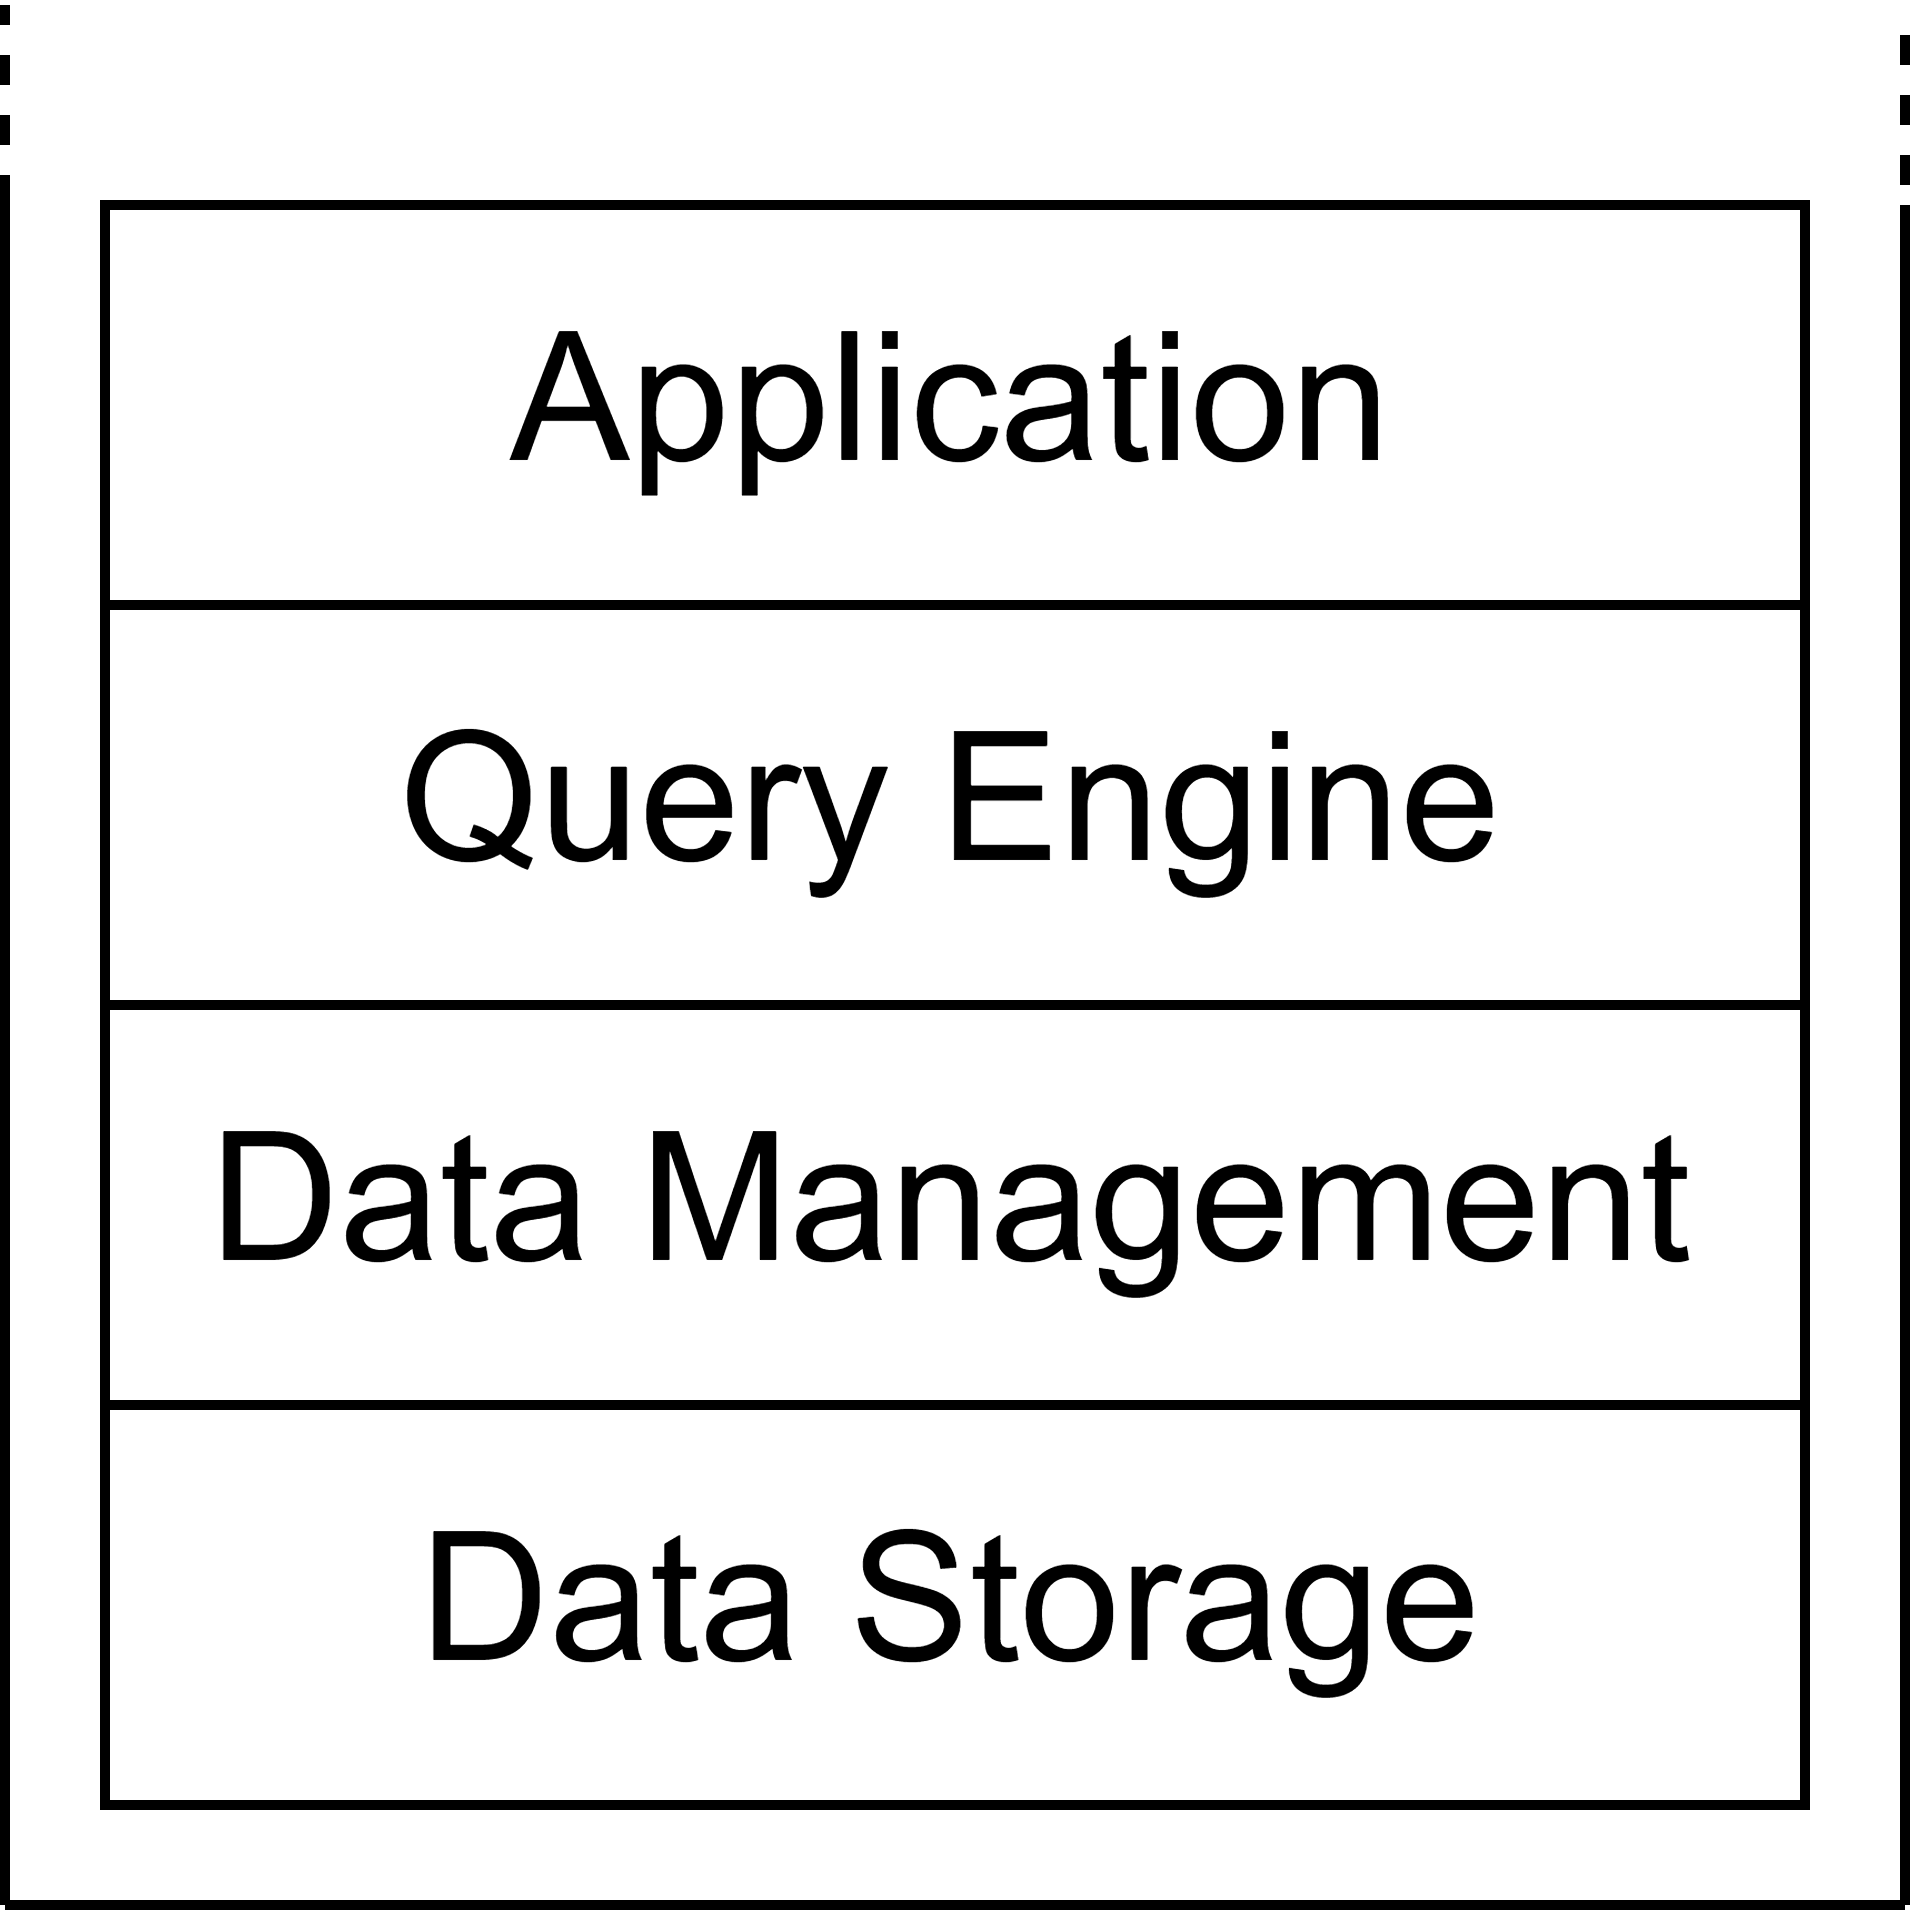
\includegraphics[width=0.4\textwidth]{figures/2-background_and_related_work/datastack.png}
    \end{center}
    \caption[Data stack abstraction]{Data stack abstraction for this project.}
    \label{fig:datastack}
\end{figure}

The data stack and this chapter are divided into four Sections:
\begin{enumerate}
    \item \textbf{Data Storage}: handles the physical storage of data. This layer determines how data is physically stored, including aspects like centralization or distribution, on-premise or cloud deployment, and storage formats such as files, objects, or blocks.
    \item \textbf{Data Management}: handles the organization, governance, and lifecycle of data. The data management layer may provide features such as \gls{ACID} properties, data versioning, support for open data formats, and the ability to store and manage both structured and unstructured data effectively.
    \item \textbf{Query Engine}: handles the execution of data queries. This layer is responsible for efficiently accessing, retrieving, and writing data based on user requests. Key features of a query engine may include caching mechanisms, highly scalable architectures, and support for diverse programming languages through \glspl{API}.
    \item \textbf{Application}: a system that utilizes the capabilities of the underlying data stack to achieve specific objectives. In this project, the focus will be on the Hopsworks feature store software.
\end{enumerate}

Following the data stack section, the architectures of the legacy system, IcedHops, and the delta-rs system architectures are explained in Section~\ref{sec:back_system_architecture}, showing how the technologies are reflected within the pipelines measured during this thesis' experiments.

\section{Data storage}
    \label{sec:back_data_storage}
    This Section describes first what data storage is and which typologies of storage exist. Thus, this project's data storage layer, \gls{HopsFS}, is presented, starting from its evolution from \gls{HDFS}, going into the details about its tools, and ending with possible alternatives, the cloud object storages.

\subsection{Block storage vs. File storage vs. Object storage}
\label{subsec:block_vs_file_vs_object}

Data can be stored and organized in physical storages, such as \glspl{HDD} or \glspl{SSD}. The three main type of data storage are (1)~Block storage, (2)~File storage, and (3)~Object storage briefly compared in Table \ref{tab:short_storage_comparison}. Each typology is describe in the following paragraphs, and their pros and cons are summarized in Table \ref{tab:long_storage_comparison}. This Subsection is a re-elaboration of three articles from major cloud providers (Amazon, Google, and IBM) \cite{BlockVsFile, HowObjectVs, ObjectVsFile2021} according to the author's understanding.

\begin{table}[!ht]
    \begin{center}
      \caption[Data storage features comparison]{Data storage features comparison. Table inspired by major cloud providers articles \cite{BlockVsFile,HowObjectVs,ObjectVsFile2021}.}
      \label{tab:short_storage_comparison}
      \begin{tabular}{cccc}
        \toprule
        \textbf{Characteristics} & \textbf{Block Storage} & \textbf{File Storage} & \textbf{Object Storage}\\
        \midrule
        Performance & High & High & Low\\
        Scalability & Low & Low & High\\
        Cost & High & High & Low\\
        \bottomrule
      \end{tabular}
    \end{center}
\end{table}

\subsubsection*{Block Storage}

Block storage is a data storage method that divides data into discrete blocks of fixed size, each assigned a unique identifier. These blocks are stored independently on a storage system, such as a \gls{SAN} or within a cloud environment. 

This decentralized approach offers several key advantages. Firstly, it enables high performance with fast read/write speeds and low latency, crucial for demanding applications like databases and virtual machine environments. Secondly, block storage provides direct, low-level access to storage volumes, similar to physical disks, granting users and applications granular control over data organization and management. This flexibility allows for a wide range of use cases, including powering virtual machine environments, supporting high-performance databases, and enabling efficient file sharing.

While offering significant benefits, block storage also presents certain limitations. It typically requires specialized hardware and infrastructure, potentially leading to higher costs compared to other storage options. Furthermore, while it offers a degree of scalability, expanding beyond certain limits can become complex and costly. Despite these considerations, block storage remains a vital technology for modern IT environments, enabling high performance, flexibility, and agility in data management.

\subsubsection*{File Storage}

File storage is a hierarchical data organization method that stores data in files, which are organized into folders within a structure of directories and subdirectories. Files are characterized by extensions (e.g., ".txt", ".png", ".csv"), defining how the data is organized and accessed. This system simplifies locating and retrieving individual files when their exact paths are known, making it intuitive and user-friendly.

This structure is particularly beneficial for managing structured data and is widely used in \gls{PC} and \gls{NAS} devices. It enables centralized file sharing on  \gls{LAN} and supports common file-level protocols, ensuring compatibility across Windows and Linux systems. Storing data on a separate NAS device or in the cloud also enhances data protection and disaster recovery, with options to replicate data across multiple geographic locations for added security.

However, as the volume of files grows, scaling becomes challenging. Locating files in a large hierarchy can be time-consuming, and scaling often requires investing in additional or higher-capacity hardware. Cloud-based file storage services mitigate these challenges by offering scalable, off-site storage managed by service providers. These services eliminate hardware maintenance costs and provide flexible, subscription-based models that adapt to varying storage and performance needs.

File storage remains popular for applications requiring simplicity and centralized access, such as file sharing, personal storage, and cloud-based platforms like Dropbox and Google Drive. While other storage solutions may be better suited for managing massive datasets or unstructured data, file storage's accessibility, affordability, and ease of use ensure its ongoing relevance.

\subsubsection*{Object Storage}

Object storage is a flat data storage method that organizes data into self-contained objects, each containing metadata that describes attributes like size, creation date, and unique identifiers. This metadata not only defines the data but also enables efficient querying and retrieval of large datasets. This makes object storage particularly well-suited for managing unstructured data, such as videos, images, and other media files that do not fit neatly into traditional hierarchical systems.

The flat structure of object storage eliminates complex hierarchies like folders and directories, simplifying organization and improving scalability. This structure allows object storage systems to replicate data across multiple regions, enhancing accessibility and fault tolerance in case of hardware failures. As a result, users benefit from faster data access in different parts of the world and robust disaster recovery options.

However, object storage has limitations. Objects are immutable, meaning they cannot be directly altered once created. Any changes require the creation of a new object. Additionally, object storage does not support transactional operations, as it lacks mechanisms like file locking, making it unsuitable for applications requiring frequent updates or real-time data changes. It also has slower writing performance compared to file or block storage solutions.

Overall, object storage is an excellent choice for use cases requiring high scalability, such as social networks, video streaming platforms, and cloud-based services. Its flat structure and metadata-driven design are ideal for managing large, static datasets. However, other storage options are preferred when high performance is required for frequently changing files or when transactional consistency is critical.

\begin{table}[h!]
    \centering
    \caption[Data storage pros and cons comparison]{Data storage pros and cons comparison. Table inspired by major cloud providers articles \cite{BlockVsFile,HowObjectVs,ObjectVsFile2021}.}
    \label{tab:long_storage_comparison}
    \begin{tabular}{|p{1.8cm}|p{4.8cm}|p{5.3cm}|}
        \hline
        \textbf{Storage Typology} & \textbf{Pros} & \textbf{Cons} \\
        \hline
        Block & 
        \begin{tabular}[t]{@{}l@{}}
            High performance \\ 
            High reliability \\ 
            Easy updates
        \end{tabular} & 
        \begin{tabular}[t]{@{}l@{}}
            Lacks metadata \\ 
            Not easily searchable \\ 
            High cost
        \end{tabular} \\
        \hline
        File & 
        \begin{tabular}[t]{@{}l@{}}
            Easy on small-scale \\ 
            User-friendly \\ 
            User-manageable \\ 
            File-level locking
        \end{tabular} & 
        \begin{tabular}[t]{@{}l@{}}
            Inefficient on unstructured data \\ 
            Limited scalability
        \end{tabular} \\
        \hline
        Object & 
        \begin{tabular}[t]{@{}l@{}}
            Ideal on unstructured data \\ 
            Cost-effective \\ 
            Highly scalable \\ 
            Efficient advanced retrieval \\ 
        \end{tabular} & 
        \begin{tabular}[t]{@{}l@{}}
            No file-level locking \\ 
            Low performance \\ 
            No data updates
        \end{tabular} \\
        \hline
    \end{tabular}
\end{table}

\subsection{\glsfmtlong{HDFS}}
% Restart from
\gls{HDFS}, a distributed file system~\footnote{\gls{HDFS} official guide available at \url{https://hadoop.apache.org/docs/r1.2.1/hdfs_user_guide.html}}, is designed to store and process massive datasets efficiently. It leverages a cluster of commodity hardware, allowing for cost-effective scalability and high availability. Unlike traditional file systems, \gls{HDFS} prioritizes high-throughput data access, making it well-suited for applications that process large volumes of data (higher than 100 GB), such as log analysis, data warehousing, and machine learning \cite{kalakarunReviewHadoopHDFS2013}.

At the core of \gls{HDFS} lies a master-slave architecture. A single Namenode acts as the central control point, managing the file system namespace, tracking file metadata, and controlling client access to files. Multiple Datanodes serve as worker nodes, each responsible for storing and managing a portion of the data within the cluster. \gls{HDFS} divides files into large blocks, which are then replicated across multiple Datanodes to ensure data redundancy and fault tolerance. This distributed storage approach enhances data availability and minimizes the risk of data loss due to hardware failures. Figure \ref{fig:hdfs_schema} presents a simplified visual representation of the Namenode read/write operations and Datanode orchestrating operations in \gls{HDFS}.

The Namenode maintains a comprehensive record of the file system namespace, including file locations, block mappings, and access permissions. This metadata is crucial for efficient data retrieval and processing. By strategically placing data replicas across different nodes, \gls{HDFS} minimizes data movement, optimizing performance and reducing network congestion. This aligns with the core principle that "moving computation is cheaper than moving data". \gls{HDFS} is designed for applications that primarily require write-once-read-many access patterns. This design choice simplifies data management and optimizes performance for batch processing tasks, where data is typically written once and then read multiple times for analysis or processing.

Furthermore, \gls{HDFS} relaxes some of the strict requirements defined by POSIX, such as low-latency access, to prioritize high-throughput data transfer. This allows \gls{HDFS} to efficiently handle large-scale data processing tasks, making it a cornerstone of many big data applications.

\begin{figure}[!ht]
    \begin{center}
      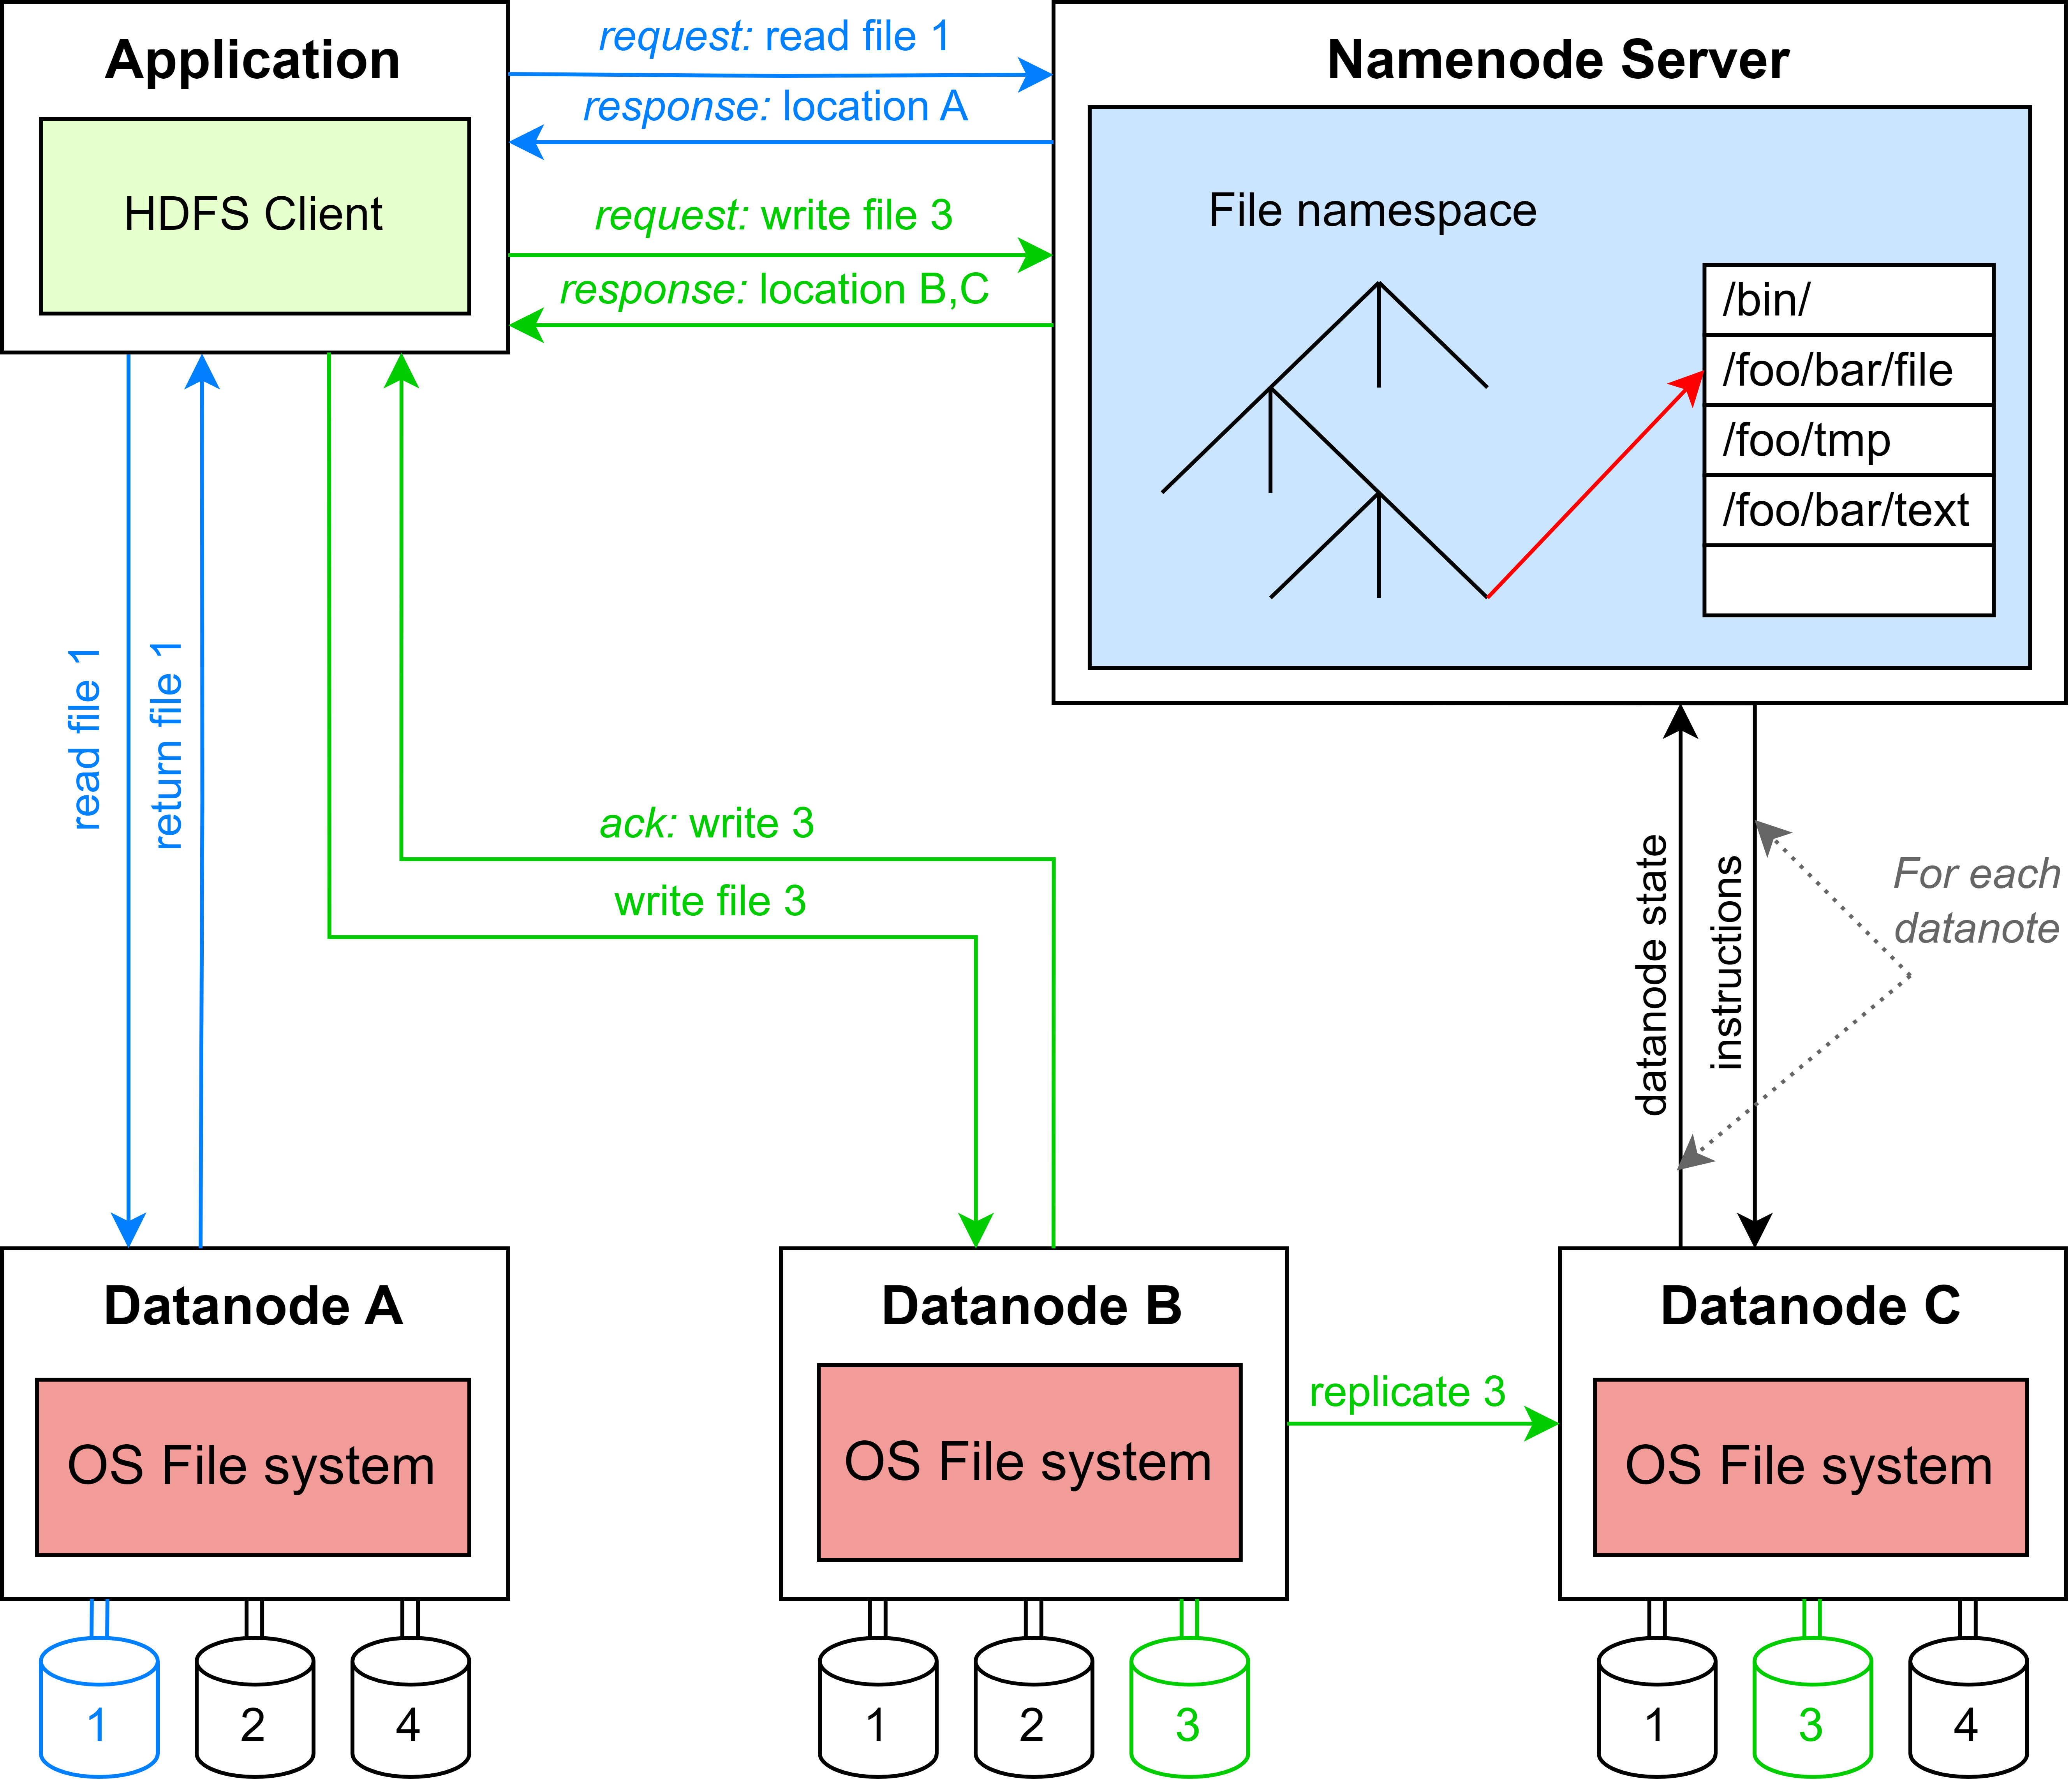
\includegraphics[width=\textwidth]{figures/2-background_and_related_work/hdfs_schema.png}
    \end{center}
    \caption[Hadoop Distributed File System architecture]{\glsentryfull{HDFS} architecture displaying in different colors basic operations: read (blue), write (green) and Namenode-Datanodes management messages (black). Note: for representation simplicity, files are not segmented into blocks and a single Namenode-Datanode message exchange is pictured. Diagram inspired by the Data-intensive Computing lectures at KTH by Prof. A. H. Payberah. Course website available at \url{https://www.kth.se/student/kurser/kurs/ID2221?l=en}.}
    \label{fig:hdfs_schema}
\end{figure}

\subsection{\glsfmtshort{HopsFS}}

\gls{HopsFS}, introduced at the 15th USENIX Conference in 2017 \cite{niaziHopsFSScalingHierarchical2017}, represents a significant evolution of \gls{HDFS}. \gls{HopsFS} addresses the critical scalability and metadata management limitations inherent to its predecessor, decentralizing metadata management by leveraging RonDB~\footnote{Details available at \url{https://www.rondb.com}}, a distributed NewSQL database, which allows metadata to be stored and managed across multiple Namenodes. This architecture supports Namenode replication and dynamic scaling, significantly enhancing throughput and operational efficiency.

\gls{HopsFS} encapsulates file system operations as distributed transactions, using advanced NewSQL features such as partition pruning and write-ahead caching. These techniques enable faster metadata retrieval and scalable operations, as seen in experiments where \gls{HopsFS} outperformed \gls{HDFS} by 16 to 37 times in throughput for real-world workloads \cite{10.1145/3626246.3653389}. Despite its scalability and performance advantages, \gls{HopsFS} remains backward-compatible with \gls{HDFS}, serving as a drop-in replacement. While \gls{HDFS} is widely adopted as a cornerstone of big data applications, \gls{HopsFS} provides a forward-looking solution for environments where metadata scalability and performance are critical. Both systems demonstrate the strengths of distributed file systems in managing massive datasets, but \gls{HopsFS} builds on the foundation of \gls{HDFS} by addressing its limitations and pushing the boundaries of what distributed file systems can achieve.

\subsection{Cloud object stores, an alternative}
The advent of cloud computing has revolutionized data storage, with object storage emerging as a dominant paradigm \cite{wuCloudStorageInfrastructure2010}. Pioneered by \gls{AWS} with its S3 service in 2006, cloud object storage services have rapidly proliferated, offered by major providers like \gls{GCS} and Microsoft Azure. This widespread adoption stems from the inherent advantages of cloud-based solutions, particularly their scalability and cost-effiency, as explained in \ref{subsec:block_vs_file_vs_object}. Cloud object storage empowers users to dynamically scale their storage capacity on-demand, paying only for the resources consumed. This pay-as-you-go model eliminates the need for significant upfront investments in hardware and infrastructure, significantly reducing operational costs. Furthermore, cloud providers leverage economies of scale to unparalleled levels of availability and scalability that are difficult to achieve for most organizations.

\gls{HDFS}, initially released in 2006, evolved alongside the rise of cloud object storage. While \gls{HDFS} has been widely adopted for on-premise deployments, the increasing popularity of cloud services has shifted the landscape. Cloud object storage solutions like \gls{AWS} S3, \gls{GCS}, and Azure Blob Storage have gained significant traction, with applications prioritizing support for these platforms due to their widespread adoption. While \gls{HDFS} and its advancements, such as \gls{HopsFS}, still have their place in specific use cases, the convenience and scalability offered by cloud object storage services have made them the preferred choice for many organizations. However, in the latest year, hybrid solution have been created, to extend cloud object storage with typical file-based system advantages, such has \gls{HopsFS}--S3 \cite{ismailHopsFSS3ExtendingObject2020}.

\section{Data management}
    \label{sec:back_data_management}
    This Section introduces the concept of data mananagement layer, starting from its origin and evolution in to today's technologies. This dissertation includes advantages and limitations of each evolutive step, and describe the functions of \gls{DBMS}. what a data storage is and which typologies of storages exist. The Subsections \ref{subsec:datalakehouse_architecture} focuses on the architecture of data lakehouses, explaing in details each component involed. Then, in Subsections \ref{subsec:datalakehouse_comparison}, three data lakehouse frameworks are compared, namely Hudi, employed in the legacy version of Hopsworks feature store, Iceberg and Delta Lake, the two alternatives evaluated.

\subsection{Brief history of \glsfmtlongpl{DBMS}}
\label{subsec:history_DBMS}
Since the 2010s, with the advent of Big Data, the data volume, variety, and production velocity have increased exponentially \cite{ederUnstructuredData802008, penceWhatBigData2014}. While on one side, this proved to be of enormous value, on the other this posed several challenges \cite{demchenkoAddressingBigData2012} on data architectures, which had to evolve to cope with these new needs. Data lakehouse frameworks, like Hudi, Iceberg and Delta Lake \cite{rajaperumalUberEngineeringIncremental2017,IcebergExamples2024,armbrustDeltaLakeHighperformance2020} are the last step of this evolution. However, to truly understand this tools, it is needed to start from the beginning of \gls{DBMS} evolution.

\smallskip

Before big data, companies already wanted to get insights from their data, automating the workflow from the data sources to point of access to this dataa. Here is where \gls{ETL} and relational databases first came into use. An \gls{ETL} pipeline consists of three steps:
\begin{enumerate}
    \item \textbf{Extracts} data from \glspl{API} or other various data sources.
    \item \textbf{Transforms} data according to one or more goal. Often this means removing absent fields, standardizes to a specific format to match the database schema, and validates the data.
    \item \textbf{Loads} it into a relational database (e.g., MySQL).
\end{enumerate}
This workflow structure enabled companies to generate \gls{BI} insights and data reports based on organizational data. However, a key limitation of this approach is its restricted ability to perform analytical queries that require joining multiple tables and working on several data dimensions. These types of queries, while executed less frequently than simpler queries, are essential for strategic decision-making (e.g., identifying the customer segment with the highest profitability over the past year, with the capabilities of drilling down on products, marketing and sales information).

\smallskip

To address the increasing demand for analytical queries, more advanced \glspl{DBMS} replaced traditional relational databases, optimizing performance for business-oriented analytical workloads. These systems, known as \glspl{OLAP}, introduced specialized storage and query execution strategies tailored for large-scale analytical processing. The most notable example of an \gls{OLAP} system is the data warehouse, which revolutionized how organizations handle structured data analysis. A data warehouse workflow, enables companies to process and analyze significantly larger datasets than traditional databases. Unlike transactional databases, which optimize for rapid insert/update operations, data warehouses focus on read-optimized queries by structuring data into columnar formats, reducing scan times for analytical queries. They maintain core relational database properties such as \gls{ACID} transactions and data versioning, ensuring data integrity and consistency for complex business intelligence applications.  

\smallskip

Over time, the exponential growth of unstructured data (e.g., images, videos, logs, and sensor data), posed new challenges for companies aiming to leverage such information. Traditional data warehouses struggled to accommodate this data due to their rigid schema requirements and high storage costs. Moreover, they were not designed to support \gls{AI}/\gls{ML} workflows that rely on diverse, unstructured datasets. To overcome these limitations, organizations adopted a new paradigm known as data lakes. Data lakes leverage cost-efficient object storage (Section~\ref{subsec:block_vs_file_vs_object}) and a schema-on-read approach, where raw data is loaded first and transformed only when needed. This shift from the traditional \gls{ETL} model to \gls{ELT} offers greater flexibility in handling diverse data types. For example, businesses can use data lakes to store raw IoT sensor readings and later refine them for predictive maintenance models, once the needed data transformation will be designed. Despite reducing storage costs and improving flexibility, data lakes introduced new complexities. Unlike structured databases, querying data lakes directly for \gls{BI} reports is impractical, as they lack indexing and transactional consistency. Additionally, maintaining separate storage solutions for structured (data warehouses) and unstructured (data lakes) data increases operational complexity and costs. A major drawback of data lakes is the risk of becoming "data swamps", repositories filled with ungoverned, low-quality data that provide little business value. Recognizing these challenges, organizations sought a hybrid solution combining the best features of data warehouses and data lakes. This led to the emergence of the data lakehouse architecture. First described by Databricks in 2020 at \gls{CIDR} \cite{lakehouse2021}, data lakehouses integrate structured and unstructured data storage capabilities of data lakes, while maintaining the governance, \gls{ACID} compliance, and indexing capabilities of data warehouses. The data lakehouse approach resolves many pain points associated with separate data warehouses and data lakes. It enables organizations to use a single storage for all types of data, while supporting high-performance \gls{SQL} queries and \gls{ML} workloads. Furthermore, by leveraging open file formats like Apache Parquet, ORC and Avro, data lakehouses ensure interoperability with various analytics engines, avoiding the risk of getting data locked into a proprietary format \cite{mazumdarDataLakehouseData2023}. All these capabilities and features make lakehouses an ideal solution for enterprise-scale data processing. Table \ref{tbl:DBMS_comparison} provides a comparison of data warehouses, data lakes, and data lakehouses, highlighting key takeaways for each technology and summarizing what described so far.


\subsection{Data lakehouse architecture}
\label{subsec:datalakehouse_architecture}
Data lakehouse architectures combines the desirable attributes of data warehouses and data lakes, mitigating the challenges encountered by both these technologies, and eliminate the need of a two-tier data stacks to run varying analytical workloads. The key components of data lakehouses are at the bases of any other architecture seen so far, but their design focus on reducing components coupling, providing more agility and choice when architecting such platform \cite{mazumdarDataLakehouseData2023}. The data lakehouse components, graphically presented in Figure \ref{fig:lakehouse_schema}, are:

\begin{itemize}
    \item \textbf{Data storage}: is where data files land after ingestion from various systems, usually a Cloud object store, as described in Section \ref{sec:back_data_storage}.
    \item \textbf{File formats}: hold the actual raw data and are phisically stored in the data storage. They are open-source file formats, such Apache Parquet or JSON, and are typically column-oriented.
    \item \textbf{Table format}: also referred as \gls{OTF}, acts as metadata layer on the top of the file formats, that abstracts the underlying physical data structure. They offers \gls{API} access to the query and storage engines.
    \item \textbf{Storage engine}: handles data management tasks, aimed at optimizing efficiency of queries over the data. It performes tasks as data compation, indexing, and partitioning.
    \item \textbf{Catalog}: sometimes described as metastore, it enables efficient search and discovery. The catalog keeps track of information about each table (name, column names, data types) and a reference to metadata for each table (table format).
    \item \textbf{Query engine}: is responsible for processing data, performing read and write operarations leveraging the table format \gls{API}. They are further explained in Section \ref{sec:back_query_engine}.
\end{itemize}

\begin{figure}[!ht]
    \begin{center}
      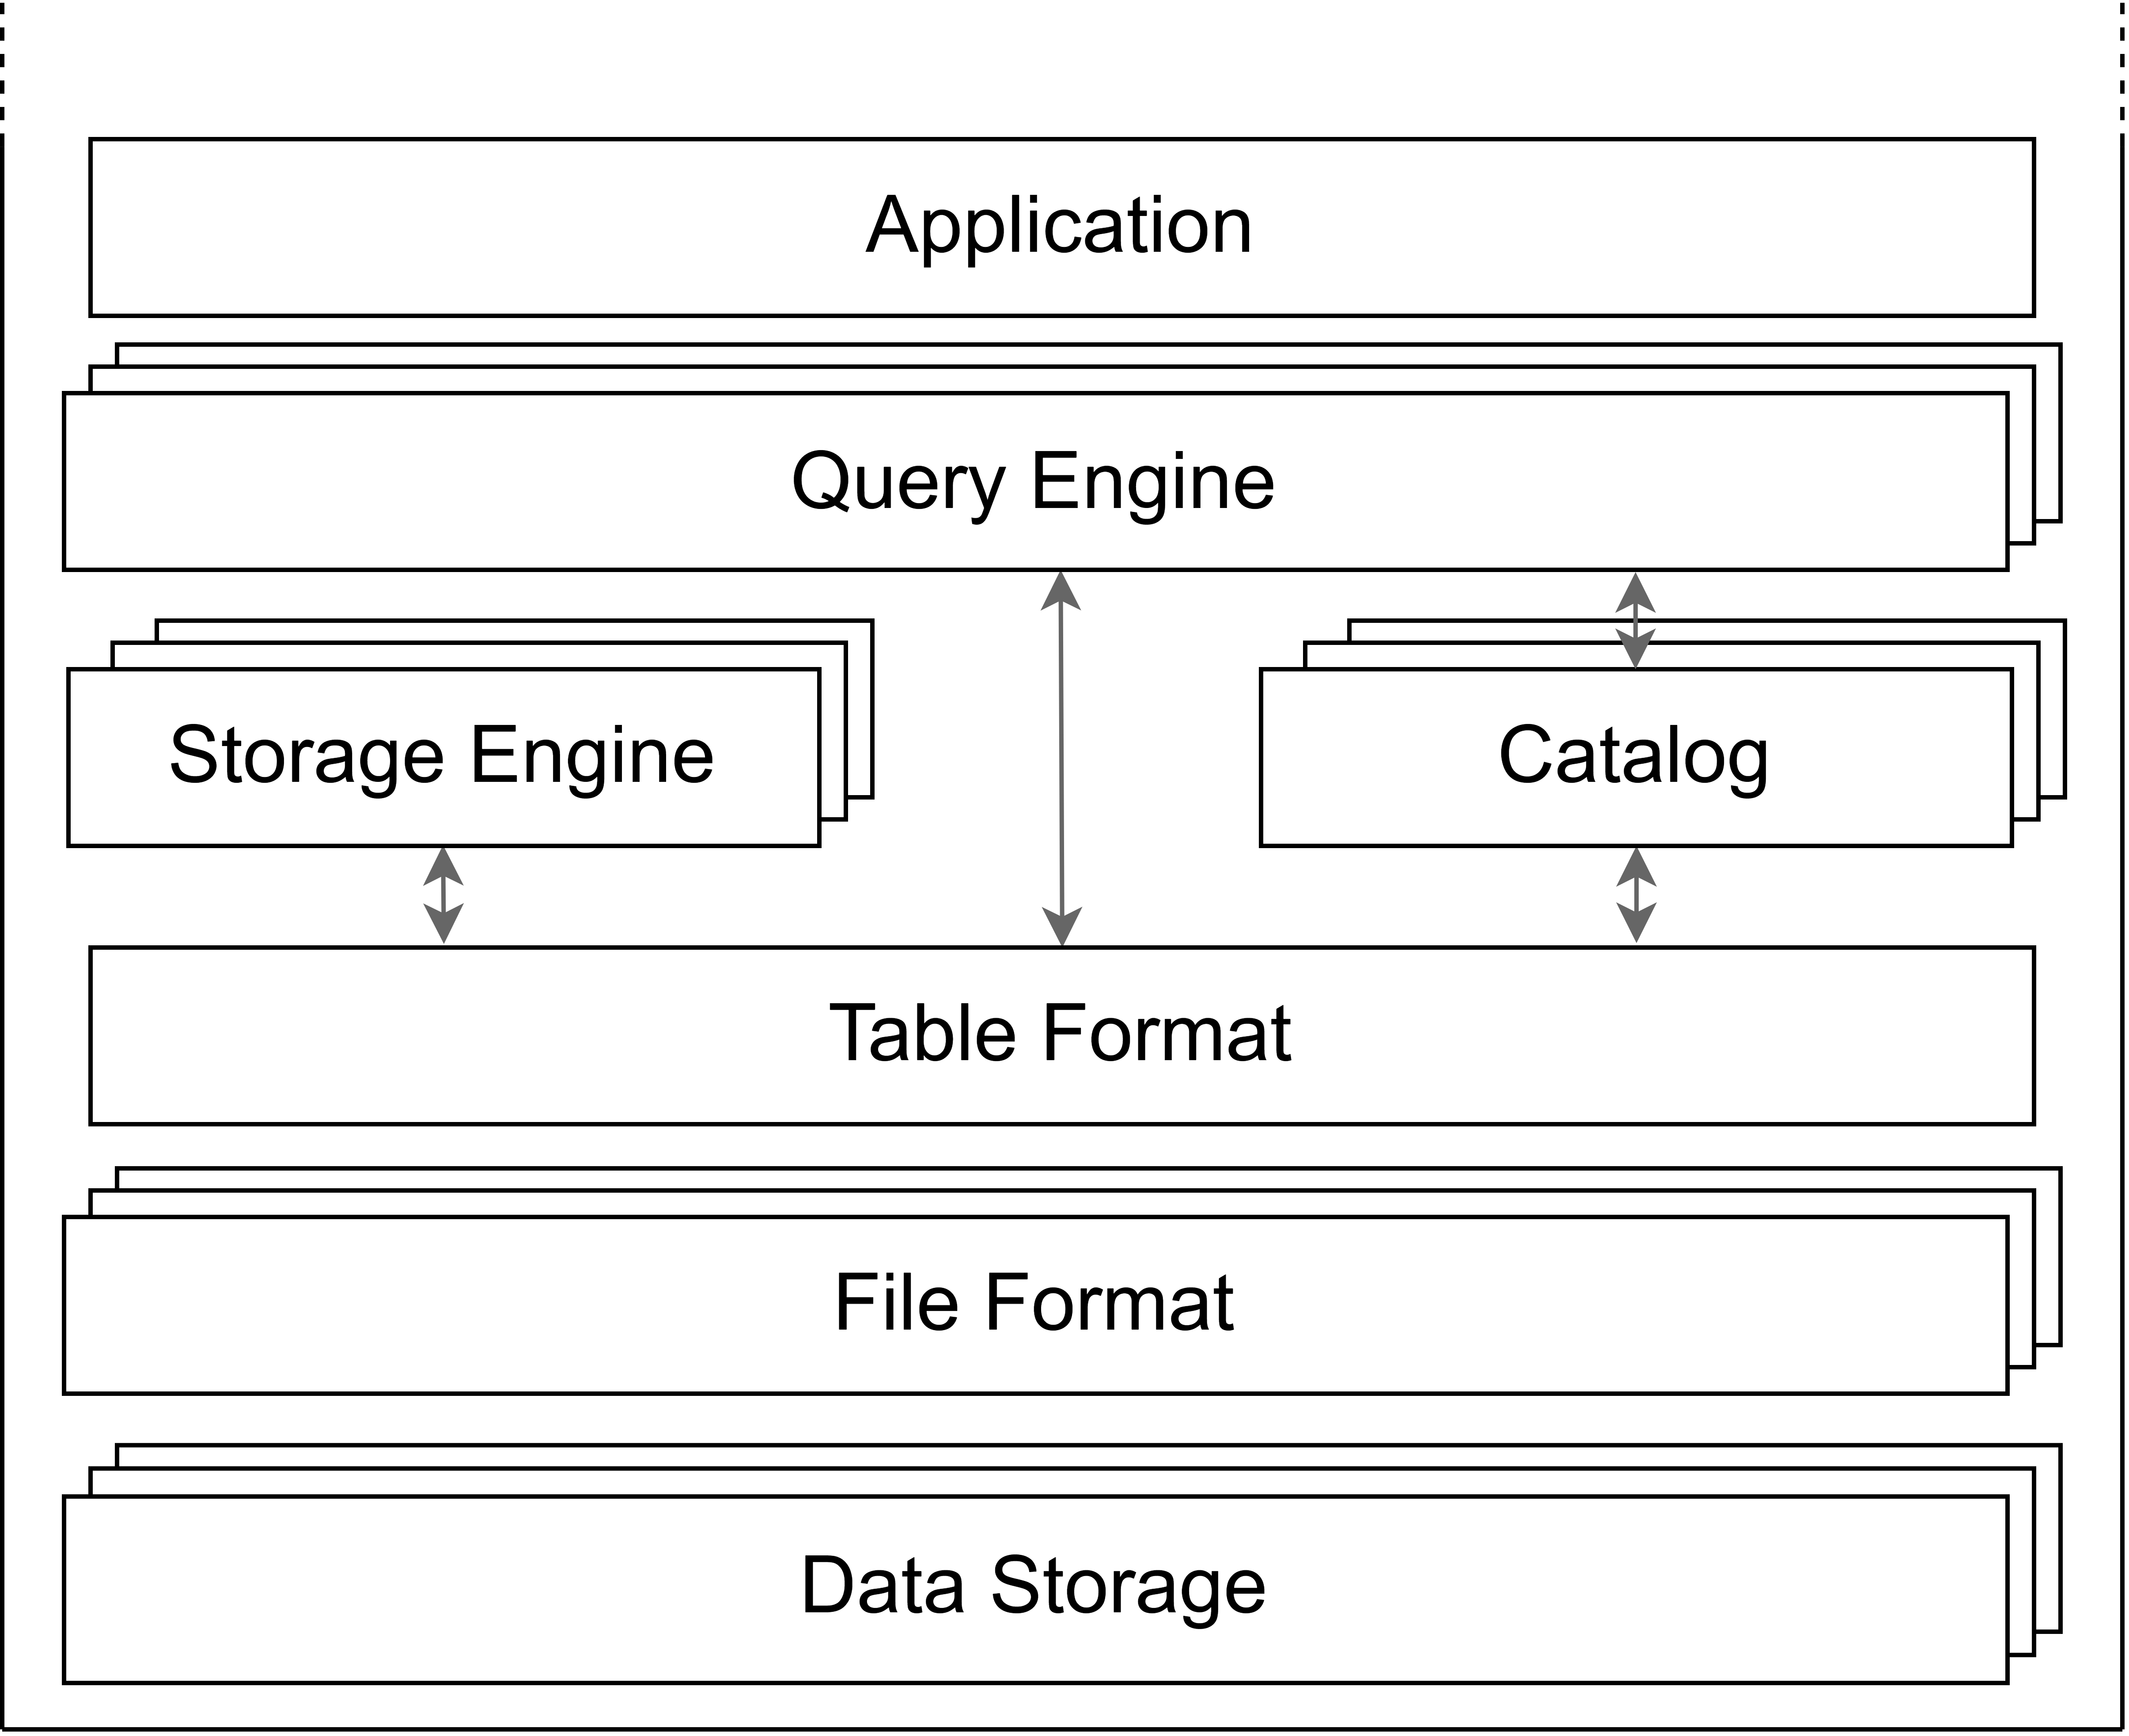
\includegraphics[width=0.6\textwidth]{figures/2-background_and_related_work/lakehouse_schema.png}
    \end{center}
    \caption[Architecture of data lakehouse]{Abstraction of architecture of a data lakehouse. Inspired by "Open table formats in perspective" article on OneHouse Website, available at \url{https://www.onehouse.ai/blog/open-table-formats-and-the-open-data-lakehouse-in-perspective}}
    \label{fig:lakehouse_schema}
\end{figure}

\gls{OTF} are open standards, and by design support interoperability throughout the stack, as visible in Figure \ref{fig:lakehouse_schema}. Thus, depending on the integration capabilities of the table format, there are several implementation options for data storage, file formats, storage engine, catalog and query engine. Additionally, recent introduction of tools like Apache XTable~\footnote{XTable repository available at \url{https://xtable.apache.org/}} demonstrates the trend towards a universal compatibility between \glspl{OTF}.


\subsubsection*{Open Table Formats}

\glspl{OTF} provide an abstraction layer on top of data lakes, enabling database-like functionalities, enhancing data management capabilities significantly \cite{lakehouse2021,DataLakehouseSurvey2025}. One of the cornerstone features of \glspl{OTF} is support for full \gls{CRUD} operations. The ability to perform updates and deletes sets datalake house data storage apart from traditional file-based storages, where such operations are cumbersome and inefficient. Performance and scalability are other notable features that \glspl{OTF} bring to the table. These formats are designed to excel in Big Data environments, where data volumes are massive and continue to grow. \glspl{OTF} could support various optimization techniques, such as indexing, partitioning, and caching, to expedite data retrieval and processing. This not only improves query performance but also ensures that the system can scale horizontally to accommodate increasing data loads without a significant degradation in performance. As a result, organizations can manage their data ecosystems more effectively, making data-driven insights more accessible and actionable. Transactional support with \gls{ACID} compliance is another key feature of \glspl{OTF}. This ensures that all data transactions are processed reliably, maintaining data integrity and consistency across the board. This is particularly important in scenarios where multiple transactions occur simultaneously or when the system needs to recover from partial failures. \glspl{OTF} guarantee that each transaction is completed successfully or fully rolled back, providing an essential level of data reliability and trustworthiness for critical business operations. This comprehensive functionality allows for flexible and complex data workflows, and ensures that data lakes and warehouses can be updated in real time, reflecting the most current state of information.



\subsection{Data lakehouse comparison}
\label{subsec:datalakehouse_comparison}

The three main data lakehouse frameworks investigated in this project are Hudi \cite{rajaperumalUberEngineeringIncremental2017}, Iceberg \cite{IcebergExamples2024} and Delta Lake \cite{armbrustDeltaLakeHighperformance2020}. Their popularity has increased proportionally with the popularity of the data lakehouse architecture, as visible by the growing community of each of these technologies in Figure \ref{fig:github_stars}, becoming the de-facto standards for data lakehouse implementations \cite{jainAnalyzingComparingLakehouse2023}. Some alternatives are newly being developed, such Apache Paimon~\footnote{GitHub repository available at \url{https://github.com/apache/paimon/}.}, but are still at early stages of their development and will not investigated in this thesis project. The following subsections present each of these technologies, specifying their development history, key features, integration capabilities, \gls{API} offered and in which are the use cases they are most suitable for.

\begin{figure}[h]
    \centering
    \begin{tikzpicture}
        \begin{axis}[
            ylabel={GitHub Stars},
            xmin=2016, xmax=2025,
            ymin=0, ymax=8000,
            xtick={2016, 2019, 2022, 2025},
            xticklabels={2016, 2019, 2022, 2025},
            ytick={1000, 2000, 3000, 4000, 5000, 6000, 7000},
            yticklabels={1k, 2k, 3k, 4k, 5k, 6k, 7k},
            legend pos=north west,
            ymajorgrids=true,
            grid style=dashed,
            width=0.9\textwidth,
            height=0.55\textwidth,
        ] 
        \addplot[color=yellow] coordinates {
            (2016, 0)
            (2019, 690)
            (2020, 1080)
            (2020.5, 1440)
            (2021, 1830)
            (2021.5, 2190)
            (2022, 2580)
            (2022.33, 2940)
            (2022.66, 3330)
            (2023, 3690)
            (2023.33, 4080)
            (2023.66, 4440)
            (2024, 4830)
            (2024.5, 5190)
            (2025, 5580)
        };
        \addlegendentry{apache/hudi}
        \addplot[color=blue] coordinates {
            (2018, 0)
            (2020, 840)
            (2021, 1320)
            (2021.5, 1770)
            (2022, 2220)
            (2022.33, 2670)
            (2022.66, 3120)
            (2023, 3600)
            (2023.25, 4050)
            (2023.50, 4500)
            (2023.75, 4950)
            (2024, 5400)
            (2024.33, 5880)
            (2024.66, 6330)
            (2025, 6780)
        };
        \addlegendentry{apache/iceberg}
        \addplot[color=red] coordinates {
            (2020, 0)
            (2021, 270)
            (2022, 450)
            (2022.5, 630)
            (2023, 780)
            (2023.2, 960)
            (2023.4, 1140)
            (2023.6, 1290)
            (2023.8, 1470)
            (2024, 1650)
            (2024.2, 1800)
            (2024.4, 1980)
            (2024.6, 2160)
            (2024.8, 2310)
            (2025, 2490)
        };
        \addlegendentry{delta-io/delta-rs}
        \end{axis}
    \end{tikzpicture}
    \caption[GitHub stars of \glspl{OTF} repositories]{Trend of GitHub stars of following repositories \url{https://github.com/apache/iceberg}, \url{https://github.com/apache/hudi}, \url{https://github.com/delta-io/delta-rs}.}
    \label{fig:github_stars}
\end{figure}

\subsubsection*{Apache Hudi}
Apache Hudi, open-sourced by Uber in 2017 \cite{rajaperumalUberEngineeringIncremental2017}, is an open-source framework that addresses the challenges of low-latency data ingestion and incremental processing. Hudi enables efficient record updates and deletions in data lakes, thus eliminating the need to rewrite entire datasets \cite{hudi_tech_docs}. The framework supports \gls{CDC} for efficient updates and deletes. Hudi offers two primary write optimization modes: \gls{CoW} for high read performance and \gls{MoR} for balancing both write and read performance. 

Hudi's metadata layer is structured around a timeline-based architecture, maintaining a history of all table operations, thus providing version control. The commit timeline records actions such as inserts, updates, deletes, and compactions, enabling time travel by referencing specific commit instants. The metadata table optimizes file listing by indexing data files, partitions, and record locations, improving query performance. Hudi also maintains delta logs (\gls{MoR}) to track incremental changes before they are compacted into columnar storage. The file groups and file slices structure organizes base and log files, ensuring efficient data versioning. 

Hudi is optimized for real-time analytics through low-latency streaming ingestion, and integrates seamlessly with Spark and Flink for data ingestion and processing. Hudi also supports reading data from Hive, Impala, and Presto. The framework incorporates multimodal indexing, such as Bloom filters and record-level indexing, and employs both Multi-Version \gls{CC} and Optimistic \gls{CC} for transaction management. Typical use cases for Hudi include streaming ingestion with frequent updates and deletes, incremental data processing, and real-time updates in domains like IoT, fintech, and log data processing \cite{comparison1_LakeFS}. While Hudi excels in real-time ingestion, its metadata overhead can be significant for large-scale analytical queries, potentially resulting in slower query performance compared to other formats like Iceberg and Delta Lake \cite{comparison4_starburst}.

Hudi's core implementation is in Java, and it integrates deeply with Apache Spark, offering a Spark datasource \gls{API} for reading and writing Hudi tables.  This makes Java and Scala the primary languages for Hudi development and usage.  While a standalone Python \gls{SDK} for Hudi doesn't exist, Python users can still interact with Hudi tables through PySpark, leveraging the Spark \gls{API}.  Although community-driven efforts like hudi-rs~\footnote{hudi-rs repository available at \url{https://github.com/apache/hudi-rs}.}, a native Rust implementation with Python bindings, are emerging, offering read support for some technologies, Hudi is currently still \gls{JVM}-centric.



\subsubsection*{Apache Iceberg}
Apache Iceberg, open-sourced by Netflix in 2018 \cite{IcebergExamples2024}, is an open-source framework that addresses the limitations of Hive tables by emphasizing scalability and correctness for large-scale analytics. By separating metadata from data, Iceberg supports efficient snapshot-based isolation and query planning \cite{shiranApacheIcebergDefinitive2024,iceberg_tech_docs}. The framework provides full \gls{ACID} transactions, ensuring atomicity, consistency, isolation, and durability. Iceberg allows for schema evolution, enabling the addition, removal, and renaming of columns, without breaking existing queries. It also supports partition evolution, allowing changes to partitioning schemes without necessitating data rewrites. 

Iceberg's metadata layer consists of multiple components that enable efficient time travel and point-in-time query planning. The manifest list acts as an index, pointing to multiple manifest files, each of which tracks a subset of data files. These manifest files store information about data file locations, partitioning, and statistics (e.g., min/max values). The snapshot metadata records changes over time, referencing manifest lists and enabling time travel by tracking table versions. Iceberg also maintains a table metadata file, which holds high-level properties, schema, partitioning details, and references to the latest snapshot. 

Iceberg is designed to scale to petabyte-scale datasets with optimized metadata management using manifest files. Its architecture enables data warehouse-like functionality, leveraging cloud object storage for efficient data access. Furthermore, Iceberg supports collaboration across multiple applications with transactionally consistent access. The framework integrates with query engines like Spark, Trino, Presto, and Dremio and supports Flink for both reading and writing. Iceberg excels in read performance, particularly for tables with large numbers of partitions \cite{comparison1_LakeFS}. It is ideal for analytical workloads that involve large-scale datasets and frequent schema or partition evolution. However, Iceberg's write performance may not be as optimized for streaming scenarios compared to other formats.

Iceberg's core is written in Java, and it is heavily integrated with Apache Spark \cite{IcebergNewHadoop,iceberg_tech_docs}.  The most common way to interact with Iceberg is through SparkSQL or other query engines like Trino and Presto, which support Iceberg natively, making Java and Scala the dominant languages in these environments.  However, Iceberg offers more than just Spark bindings. PyIceberg \cite{PyIceberg} provides a direct Python interface for read and -- from release 0.6.0 in 2024 -- write operations, making Iceberg accessible to Python developers without requiring PySpark.  Furthermore, query engines like Trino, accessible from Python via libraries like PyHive, allow Python users to query Iceberg tables through \gls{SQL}. Iceberg community has recently developed a Rust implementation, iceberg-rust~\footnote{iceberg-rust available at \url{https://github.com/apache/iceberg-rust}.}, which provides read access to Iceberg tables, further expanding its accessibility to a wider range of language ecosystems.



\subsubsection*{Delta Lake}
Delta Lake, open-sourced by Databricks in 2019 \cite{armbrustDeltaLakeHighperformance2020}, is an open-source framework that enhances the reliability and performance of data lakes, facilitating a seamless transition between batch and streaming use cases. Often considered the first data lakehouse, Delta Lake employs a transaction log to record all changes to data, ensuring consistent views and write isolation, which supports concurrent data operations \cite{deltalake_tech_docs}. The framework offers \gls{ACID} transactions, as well as features such as unified batch and streaming processing, indexing, and schema enforcement.

Delta Lake's metadata layer is built around the Delta Log, which records every transaction in JSON files, enabling time travel. The transaction log maintains a sequential history of operations, while checkpoint files (stored in Parquet format) periodically summarize log entries for faster metadata access. The protocol metadata defines the table's versioning, schema, and supported features, ensuring compatibility across different readers and writers. It also incorporates metadata-informed data skipping during merge operations and supports streaming through change data feeds.

Delta Lake tighlty integrates with Spark, thus it is particularly well-suited for real-time streaming, batch processing, and \gls{ML} pipelines requiring data versioning. While its open-source adoption continues to grow, Delta Lake remains deeply integrated with the Databricks ecosystem \cite{jainAnalyzingComparingLakehouse2023,comparison2_medium_recent}. Additionally, its focus on schema and partition evolution is less pronounced compared to frameworks like Iceberg, making Delta Lake less suitable for situations where data schemas are frequently changing.

Delta Lake  core is written in Java and Scala \cite{deltalake_tech_docs}, providing native support within the Spark ecosystem through the delta package. This allows Java and Scala developers to interact directly with Delta tables. Python support is provided via PySpark, enabling Python developers to leverage the Spark \gls{API} for Delta Lake operations.  However, Delta Lake's reach extends beyond the \gls{JVM}.  With the release of Delta Kernel \cite{AnnouncingDeltaLake2023}, a Java library providing low-level access, and the development of delta-rs~\footnote{delta-rs repository available at \url{https://github.com/delta-io/delta-rs}.}, a Rust-based implementation, Delta Lake has become accessible to a wider audience.  The library delta-rs allows interaction with Delta tables without Spark or \gls{JVM} dependencies, and its Python bindings makes this particularly attractive to the Python data science community.



\medspace
In Table \ref{tbl:lakehouse_comparison} is presented a comparation between key features of the three data lakehouse frameworks.

\section{Query engine}
    \label{sec:back_query_engine}
    This section describes the technologies used to query, cache, and process data in this project. The category of query engine includes mainly Apache Spark and DuckDB, but technologies operating at the same abstraction level of those are here presented, namely Apache Kafka, Arrow Flight and SQLite. \todo{maybe add here Apache Hive.}

\subsection{Apache Spark}
Apache Spark is an open-source distributed computing framework designed for large-scale data processing~\cite{zahariaApacheSparkUnified2016}. It builds upon MapReduce, a distributed programming model developed by Google for handling massive datasets~\cite{dean2004mapreduce}, later adapted into Hadoop MapReduce by Yahoo! engineers~\cite{borthakurHadoopDistributedFile2005}. Spark enhances this model using \glspl{RDD}\cite{Zaharia:EECS-2011-82}, a disitrbuted memory abstraction that enables lazy in-memory computation, diffently by on-disk MapReduce's computation, that is tracked through lineage graphs. This increases fault tolernace \cite{Zaharia:EECS-2011-82} and allow to manage even bigger scale computations.

Spark supports various workloads beyond batch processing, leveraging an in-memory execution model for efficiency. Its core components include SparkSQL for querying structured data, Spark Streaming for real-time processing, MLlib for scalable \gls{ML}, and GraphX for large-scale graph processing. With support for iterative computations, Spark is particularly well-suited for \gls{ML} and graph analytics. It also provides \glspl{API} for Scala, Java, Python (via PySpark), and R, making it accessible to a broad range of users. Despite its advantages, Spark has limitations. Its in-memory execution requires significant RAM, and \gls{JVM}-based execution can lead to performance overhead due to garbage collection. Tuning performance involves fine-tuning configurations, which can be complex. Additionally, Spark Streaming's micro-batch processing introduces higher latency compared to other frameworks, making it not the best solution for small-scale datasets processing \cite{BenchmarkResultsSpark}.

\subsection{Apache Kafka}

Apache Kafka is a robust, open-source distributed platform for handingle data streaming, that has become a cornerstone of modern data architectures~\cite{krepsKafkaDistributedMessaging2011}. Kafka supports high throughput data ingestion and processing, making it exceptionally well-suited for handling massive volumes of data in real, given its ability to manage and process continuous streams of data with very low latency. Kafka's architecture, which emphasizes fault tolerance, scalability, and durability, allows it to handle the demands of mission-critical systems that require continuous data flow and processing. \todo{Maybe add here schema of Kafka Architecture} The key components of Kafka architecture are:

\begin{enumerate}
    \item \textbf{Producer}: an application that publishes data, labeling into specific topic that group similar messages.
    \item \textbf{ZooKeeper}: the responsible for managing the Kafka cluster, including broker(s) information and topic message tracking, tracked with an offset for each topic.
    \item \textbf{Broker}: a processing node, or server, that handles data for specific topics. It receives messages from producers and delivers them to consumers upon request, enabling asynchronous communication. When for a single topic there are multiple brokers, one is elected as a leader, and the others replicate its content.
    \item \textbf{Consumer}: an application that subscribes to specific topics to receive and process data. Multiple consumers can subscribe to the same topic.
\end{enumerate}

Kafka enables applications to behave as producers and consumers, without the need of developing any synchronization protocol. This enables producers to reach high throughput, as they can broadcast messages without waiting for any acknoledgements or availability singal from the consumers. Due to its distributed architecture, a Kafka ecosystem can be optimised according to specific needs, allowing several brokers, producers and consumers to coexist.



\subsection{Catalogs}
\label{subsec:back_catalogs}
The term catalog is used in the data domain in multiple contexts, in each of those with a different definitions. In the data lakehouse context, thus in this project context, a catalog is a technical catalog also called metastore \cite{shiranApacheIcebergDefinitive2024}. As explained in Section \ref{subsec:datalakehouse_architecture}, a catalog plays an important role in tracking tables and their metadata. It is, at a minumum, the source if truth for a table's current metadata location. This is in contrast to a federated catalog, which is a central portal for data discovery and collaboration, since it tracks datasets across multiple data stores. It focuses on business needs such data governance and documentation, and sets standards for authentication and authorisation \cite{blueCatalogsRESTCatalog2024}. A federated catalog may point to tables from Cassandra, Postgres, Hiv, and other systems.

Made clarity over the catalog definition regarding this project, there are several technologies providing such tool. When data lakehouses were first created \cite{rajaperumalUberEngineeringIncremental2017,shiranApacheIcebergDefinitive2024}, the \gls{HMS} was the most popular catalog. \gls{HMS} is the technical catalog for Hive tables, but it can actually belong to both catalog categories, since it may also track \gls{JDBC} tables, and other datasets. However, scale challenges led developers and big tech companies to develope their own more scalable tools, which contributed to the development of data lakehouses technology itself, such the case of Iceberg \cite{IcebergNewHadoop}.

Data lakehouse technologies support different Catalogs, as shown in Table \ref{table:lakehouse_comparison}. Depending on the specific business need or on the available cloud resources and ecosystem, possible "pluggable" catalogs are:
\begin{itemize}
    \item \textbf{SQLite}: is a C library, with Python bindings, that provides lightweight disk-base database, that allows accessing the database with nonstandard variants of \gls{SQL}, where metadata can be saved. This does not require a separate server process, thus it is great in embedded applications, but it is not suitable for big-scale applications.
    \item \textbf{\gls{AWS} Glue}: provides a Data Catalog that serves as a managed metastore within the \gls{AWS} ecosystem. It integrates well with other\gls{AWS} services, thus it is a common choice for data lakehouses built on \gls{AWS}.
    \item \textbf{DynamoDB}: it is primarily a No~\gls{SQL} databases that due to its scalability and performance, can be used as a metastore. This is less common compared to other options.
    \item \textbf{\gls{JDBC}}: per sé is not a catalog, but it's the standard Java \gls{API} for connecting to relational databases. In this context, \gls{JDBC} would be used to connect to and interact with database systems that stores metadata.
    \item \textbf{Nessie}: acts as a versioned metastore, providing Git-like capabilities for managing data lake tables
    \item \textbf{Databricks Unity}: is Databricks' unified governance solution, thus it is a federated catalog, which however includes also technical catalog capabilities. It provides a centralized metastore specifically designed for the Databricks Lakehouse Platform, thus is the most common option for Delta Lake-backed lakehouses \cite{AnnouncingDeltaLake2023}.
\end{itemize}

As data lakehouse frameworks grew to support more and more languages and engines, pluggable catalogs started causing some practical problems, related to compatibility. It proved indeed difficult, for commercial offerings, to support many different clients and catalog features. To overcome these problems, some developers, like Iceberg's community \cite{blueCatalogsRESTCatalog2024}, created also a REST catalog protocol, a common \gls{API} for interacting with ant catalog. The advantages of such protocol are are multiple: (1) one client implementation, for new languages or engines, can support any catalog; (2) secure table sharing is enabled, using credential vending or remote signing; (3) the amount of failures is reduced, since server-side deconfliction and retries are supported.

When implementing a new data lakehouse, the catalog decision depends on the specific integrations and feature proper of each catalog option, also considering how this can be configured on the top of the previously added layer, as shown in Table \ref{fig:lakehouse_schema}.

\subsection{Duck DB}
DuckDB \cite{raasveldtDuckDBEmbeddableAnalytical2019} is an open-source, embeddable, \gls{OLAP} \gls{DBMS} designed for efficient processing of small-scale datasets (from 1GB to 100GB) within the same process as the application using it.  This embedded, in-process operation, inspired by SQLite's success, simplifies deployment and eliminates the overhead of inter-process communication, leading to high responsiveness and low latency.  DuckDB requires no external dependencies and compiles into a single amalgamation file, enhancing portability across major operating systems and architectures, including web browsers via DuckDB-Wasm.  It offers \gls{API} for various languages, such Java, C, C++, Go, Rust and Python and supports complex \gls{SQL} queries, including window functions and \gls{ACID} properties through Multi-Version \gls{CC}.  

Data is stored in persistent, single-file databases, and secondary indexes enhance query performance.  DuckDB's columnar-vectorized query execution engine, a key design choice for \gls{OLAP} workloads, processes data in batches (vectors), significantly improving performance compared to traditional row-by-row processing systems.  While optimized for analytical queries processing significant portions of datasets, DuckDB is not designed for massive data volumes (1TB or more) that require disk-based processing, as its core processing relies on in-memory operations.  However, its extensible architecture allows for adding features like support for Parquet, JSON, and cloud storage protocols as extensions.

\subsection{Arrow Flight}
Arrow Flight is an high-performance framework designed for efficient data transfer over networks, mostly utilising Arrow tables \cite{wesmIntroducingApacheArrow2019}. This protocol facilitates the transmission of large data volumes stored in a specific format, such as Arrow tables, without the necessity of serialisation or deserialisation for transfer. This significantly accelerates the data transfer, making Arrow Flight highly efficient. Arrow Flight is engineered for cross-platform compatibility and supports many programming languages, including C++, Python, and Java. The protocol further facilitates parallelism, enhancing transmission speeds by using numerous nodes in parallel networks. The Arrow Flight protocol is constructed upon gRPC, facilitating standardisation and simplifying the construction of connectors.

\section{Application - Hopsworks}
    \label{sec:back_applications}
    This Section describes the application layer, the uppermost layer presented in Figure \ref{fig:datastack}, which takes advantage of the data stack described above. The software described is the Hopsworks feature store, which this project contributes to. This software is part of the broader \gls{MLOps} platform offered by Hopsworks AB, the company that hosted this master thesis.


\subsection{Machine Learning Operations (MLOps)}
\label{subsec:back_mlops}

\gls{MLOps} are a full set of practices related to the development and automation of \gls{ML} workflows. Through the \gls{MLOps} lenses, a \gls{ML} workflow is logically separated in smaller steps, and considered from a data, code and model perspective. Differently from a classical software application, where only the code needs versioning, in the context of \gls{ML} applications, it is key that all three of data, code and model are versioned. Perhaps, different data might be used by models in different moments, as well as new model might be trained on the same data, to truly understand their improvements.The novel challenges are thus related to data validation, \gls{ML} artifacts versioning, \gls{ML} workflow orchestration, and infrastructure management, given higher computation and storage capabilities needed by those workflows \cite{SurgeAI2024,PDFBigData2024}.

The need of the described features saw new solutions emerging, like the Hopsworks AI data platform \cite{HopsworksRealtimeAI}. In the context of data versioning, the specific solution is called feature store \cite{MeetMichelangeloUbers2017}, which consists in a centralized fast-access storage for both real-time and batch data.

A simple architecture following \gls{MLOps} principle is presented in Figure \ref{fig:mlops_hops}. As first step, data are gathered either streaming (real-time) or batch data sources. A feature pipeline process those the data, performing model-independent transformations \cite{BigDictionaryMLOps2024}, and saves them in the feature store. A training pipeline runs now model-dependent transformations on features and labels retrieved from the feature store, and train the respective model, saving the trained model in the model registry. The last pipeline, the inference pipeline, extract at its need a specific model from the model registry and access the features, over which a inference will be conducted, from the feature store. The output of this pipeline, which normally is embedded directly in the consuming application, are the predictions of the model over the selected features, altogether with logs describing the performance of the model according to a pre-selected measure. All the pipeline are decoupled and could thus work asynchronously, making the whole \gls{ML} workflow scalabile, maintainable and effective.

\begin{figure}[!ht]
    \begin{center}
      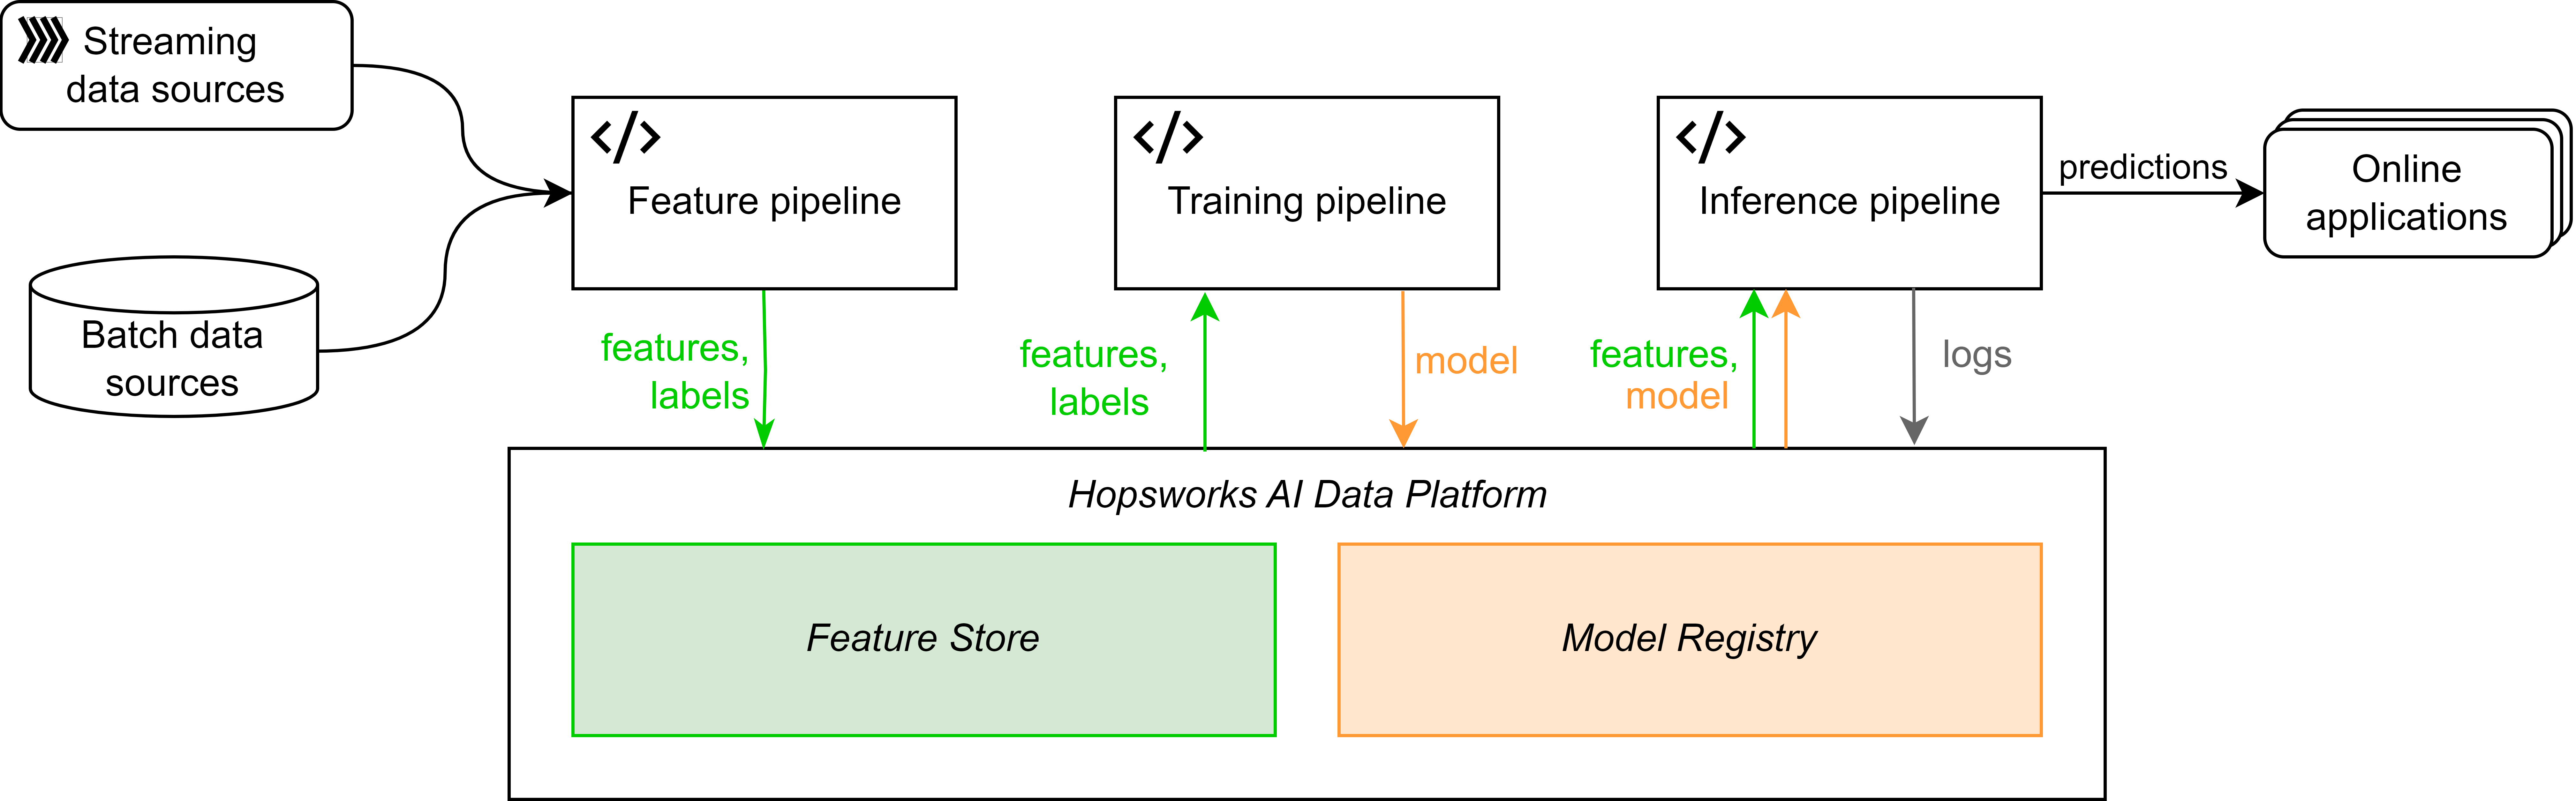
\includegraphics[width=\textwidth]{figures/2-background_and_related_work/MLOps_hops.png}
    \end{center}
    \caption[Feature store in an MLOps pipeline]{\glstext{MLOps} pipeline using a feature store and a model registry. Diagram inspired by Hopsworks documentation available at \url{https://www.hopsworks.ai/dictionary/feature-store}.}
    \label{fig:mlops_hops}
\end{figure}


\subsection{Hopsworks AI Data Platform}
\label{subsec:back_hopsworks_FS}
As briefly said above, the feature Store is a key data layer in an \gls{ML} application built over the \gls{MLOps} principles. The feature store enables feature reusability, as well as multi-user collaboration and a centralized authenticated access to the feature. The Hopsworks feature store organizes features in feature groups. Those are mutable collection of features, over which developers can perform \gls{CRUD} operations, accessing them via the Hopsworks \glspl{API}.

The Hopsworks feature store supports both batch data sources and real-time data streaming. This hybrid system is possible thanks to the dual implementation of an offline and an offline feature store. The offline feature store is a column-based storage suited for batch data that is updated with a low frequency (every few hours at maximum frequency). The online feature store, on the other hand, is a real-time row-based, key-value data storage based on RonDB, thus enabling low latency and real-time processing. To maintain consistentency between those two stacks, the Hopsworks feature store has a unique point of entry for data, which is Kafka, explained in detail in \ref{subsec:back_apache_kafka}. This guarantess that each message is delivered to both storages, which acts are consumers subscribed to the Kafka topics.

The model registry works under the same principles of the feature store, proving a centralized access and a standard deployment for all the models saved in it. It also saves information about model performance along time, model schemas and training feature logs, to ease model reproducibility and tracking.

\section{System architectures}
    \label{sec:back_system_architecture}
    This Section describes the architectures of the legacy, based on Hudi the system implemented during this thesis work, based on Iceberg, and the system implemented in a related thesis work \cite{manfrediReducingReadWrite2024}, based on Delta Lake. Those are the system that will be run and measured in teh experimental part of this thesis work. This Section is divided into six Subsections, according to the system and the operation run over it. For each Subsection, a chart presents the operation protocol step by step.



%%%% HUDI WRITE
\subsection{Legacy system - Hudi - writing}
\label{subsec:back_sys_hudi_write}

Figure \ref{fig:hudi_write}~\footnote{For enhanced visualization, refer Figure \ref{fig:appx_hudi_write_schema}.} shows the legacy Hopsworks feature store write process from the client onto the offline feature store. The process is mainly split into two synchronous parts: upload and materialization. In the upload step, the Pandas DataFrame given as input is converted into rows and sent to Kafka one row at a time. Then, when the upload is completed, the client will be notified. Asynchronously, a Spark job, the Hudi Delta Streamer, has been running in the cluster since the Hopsworks cluster was started. This job periodically retrieves messages from Kafka, and then once it retrieves a full table, it writes the table in a column-oriented format to Apache Hudi, which sits on top of a \gls{HopsFS} system. Once the materialization is completed, the Python client will be notified of completion.

As in the pipeline, the upload and the materialization are two parts of the process that do not act synchronously. During the experimental part of the thesis, the materialize function was called to measure the latency of the whole process without having to account for the Hudi Delta Streamer data retrieval period. This allows the system to perform the materialization on call instead of waiting for the period. This enabled the experiments to retrieve accurate data on the total latency of the process.

\begin{figure}
    \begin{center}
      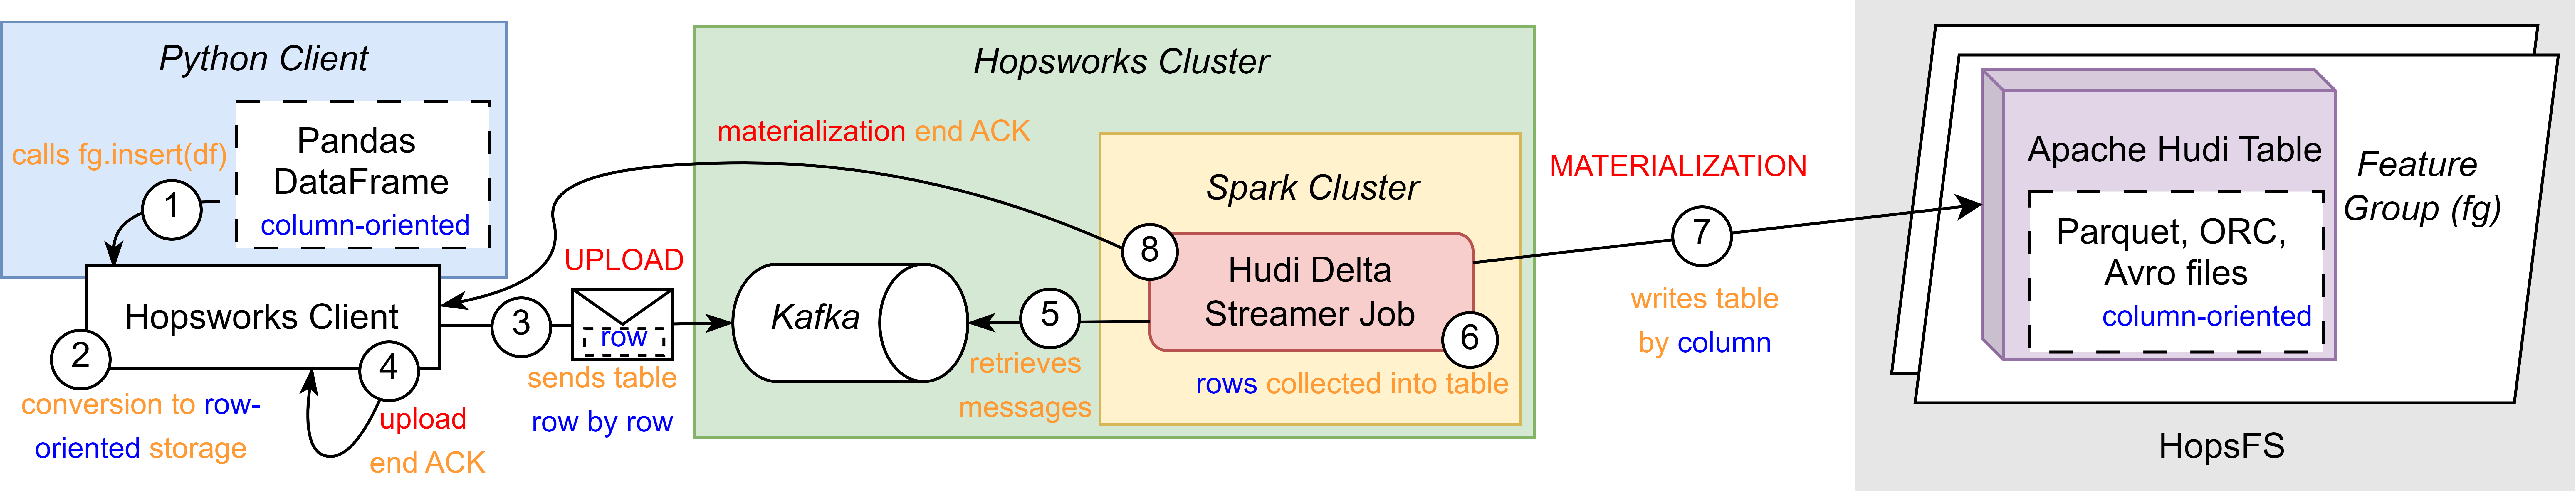
\includegraphics[width=\textwidth]{figures/2-background_and_related_work/hudi_write.png}
    \end{center}
    \caption[Legacy system - Hudi - write process]{Legacy system writing a Pandas DataFrame from a Python client to the Hopsworks offline feature store. Each step is represented with a number. The table format conversion is outlined in blue, i.e., from columns to rows and then from row to columns. Steps from one to four represent the upload process, while the materialization process is complete at step eight. The diagram was realized based on one-to-one interviews with Hopsworks AB employees developing the Hopsworks feature store.}
    \label{fig:hudi_write}
\end{figure}



%%%% HUDI READ
\subsection{Legacy system - Hudi - reading}
\label{subsec:back_sys_hudi_read}

Figure \ref{fig:hudi_read}~\footnote{For enhanced visualization, refer Figure \ref{fig:appx_hudi_reading_schema}.}  shows the offline feature store. Unlike the writing process, the process is not Spark-based and uses a Spark alternative: a combination of an Arrow Flight server and a DuckDB instance. This avoids the conversion into row-based tables for sending the data, keeping the unified standard Arrow Table, which is a column-oriented format.

\begin{figure}
    \begin{center}
      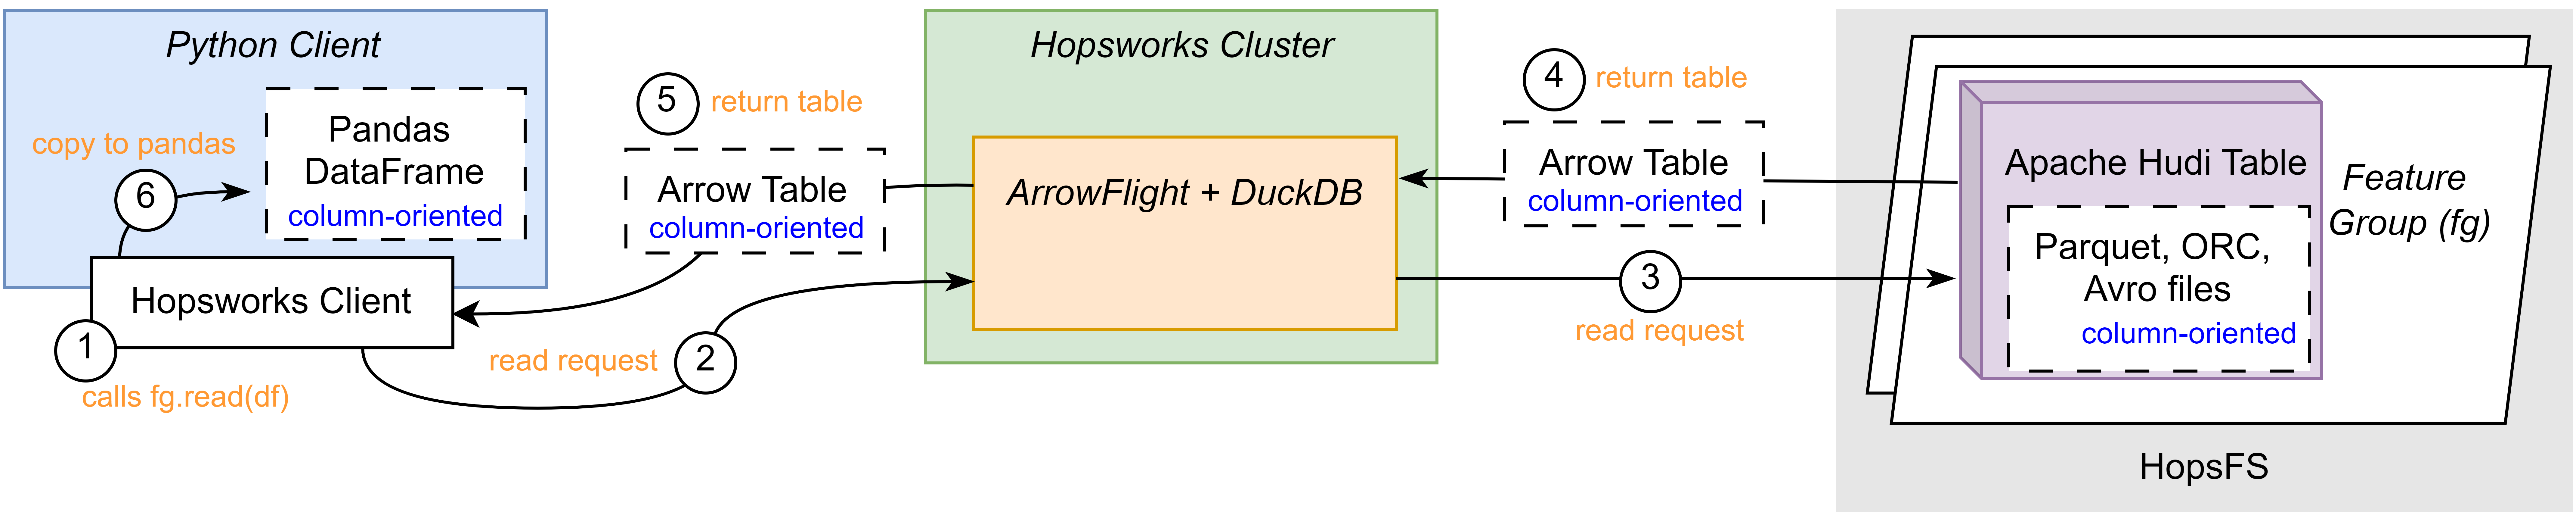
\includegraphics[width=\textwidth]{figures/2-background_and_related_work/hudi_read.png}
    \end{center}
    \caption[Legacy system - Hudi - read process]{Legacy system reading a table from the Hopsworks offline feature store and loading it into the Python client's local memory. The process is streamlined using Arrow Tables that avoid table conversion. Diagram inspired by the Hopsworks feature store paper \cite{10.1145/3626246.3653389}.}
    \label{fig:hudi_read}
\end{figure}



%%%%% ICEBERG WRITE
\subsection{New system - PyIceberg - writing}
\label{subsec:back_sys_iceberg_write}

Figure \ref{fig:iceberg_write} shows how the PyIceberg library writes on an Iceberg table instanced on top of \gls{HopsFS}. If first requests metadata information about the existing table to Iceberg Catalog, implemented using SQLite in the example. Once the JSON file containing the metadata is received, it reads the table location and request to read the table. The PyIceberg library streamlines the process without passing from a server instance (Spark), removing the middle-tier from the process.

\begin{figure}
    \begin{center}
      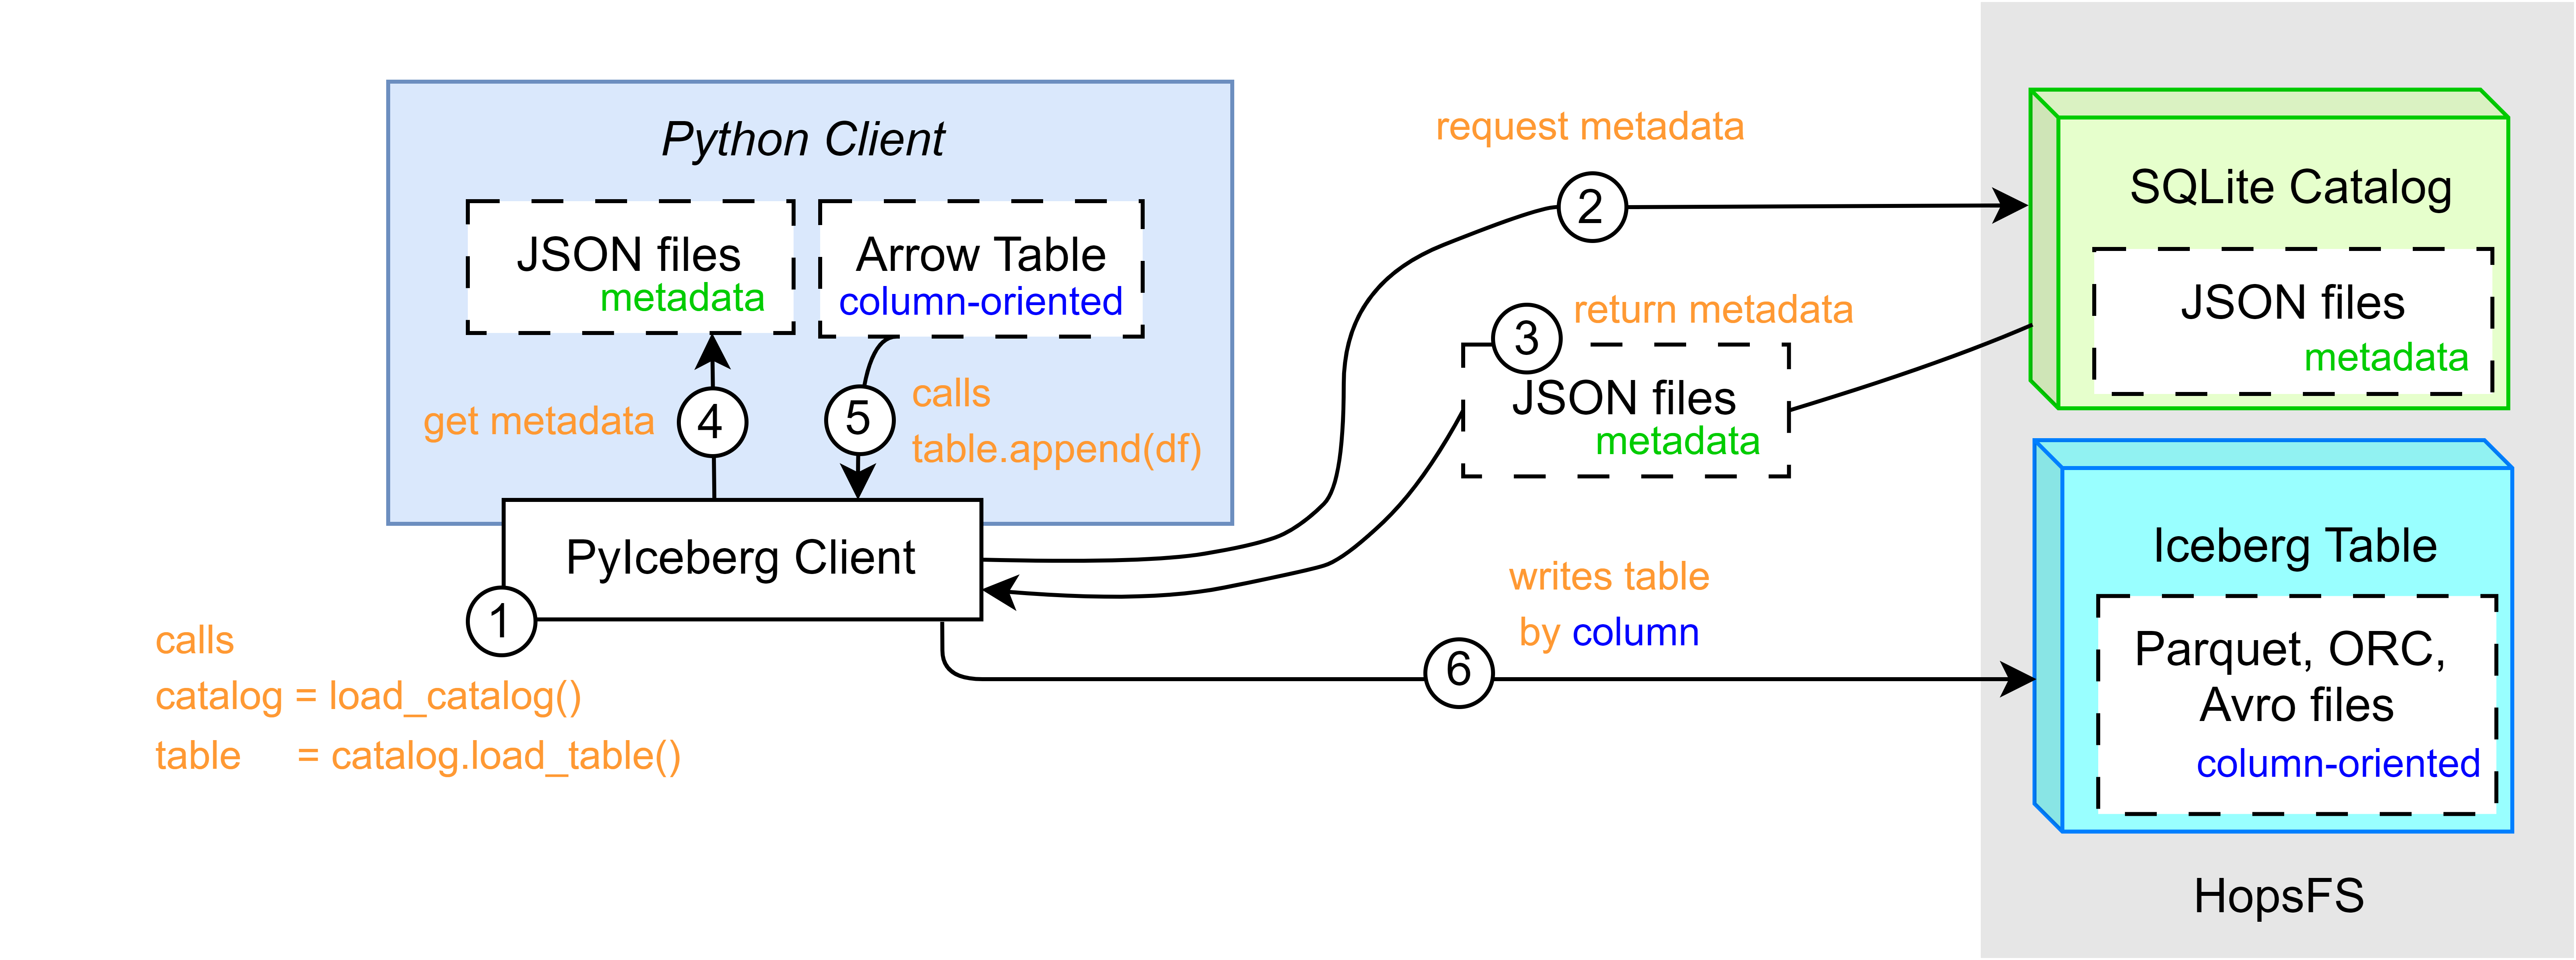
\includegraphics[width=\textwidth]{figures/2-background_and_related_work/iceberg_write.png}
    \end{center}
    \caption[New system - PyIceberg - write process]{PyIceberg library writing an Arrow Table from a Python client to an Iceberg Table stored on \gls{HopsFS}.}
    \label{fig:iceberg_write}
\end{figure}



%%%%% ICEBERG READ
\subsection{New system - PyIceberg - reading}
\label{subsec:back_sys_iceberg_read}

Figure \ref{fig:iceberg_read} shows how the PyIceberg library reads on an Iceberg table instanced on top of \gls{HopsFS}. If first requests metadata information about the existing table to Iceberg Catalog, implemented using SQLite in the example. Once the JSON file containing the metadata is received, it reads the table location and proceed to write (append), by column, on the Iceberg Table. The PyIceberg library streamlines the process without passing from a server instance (Arrow Flight), removing the middle-tier from the process.

\begin{figure}
    \begin{center}
      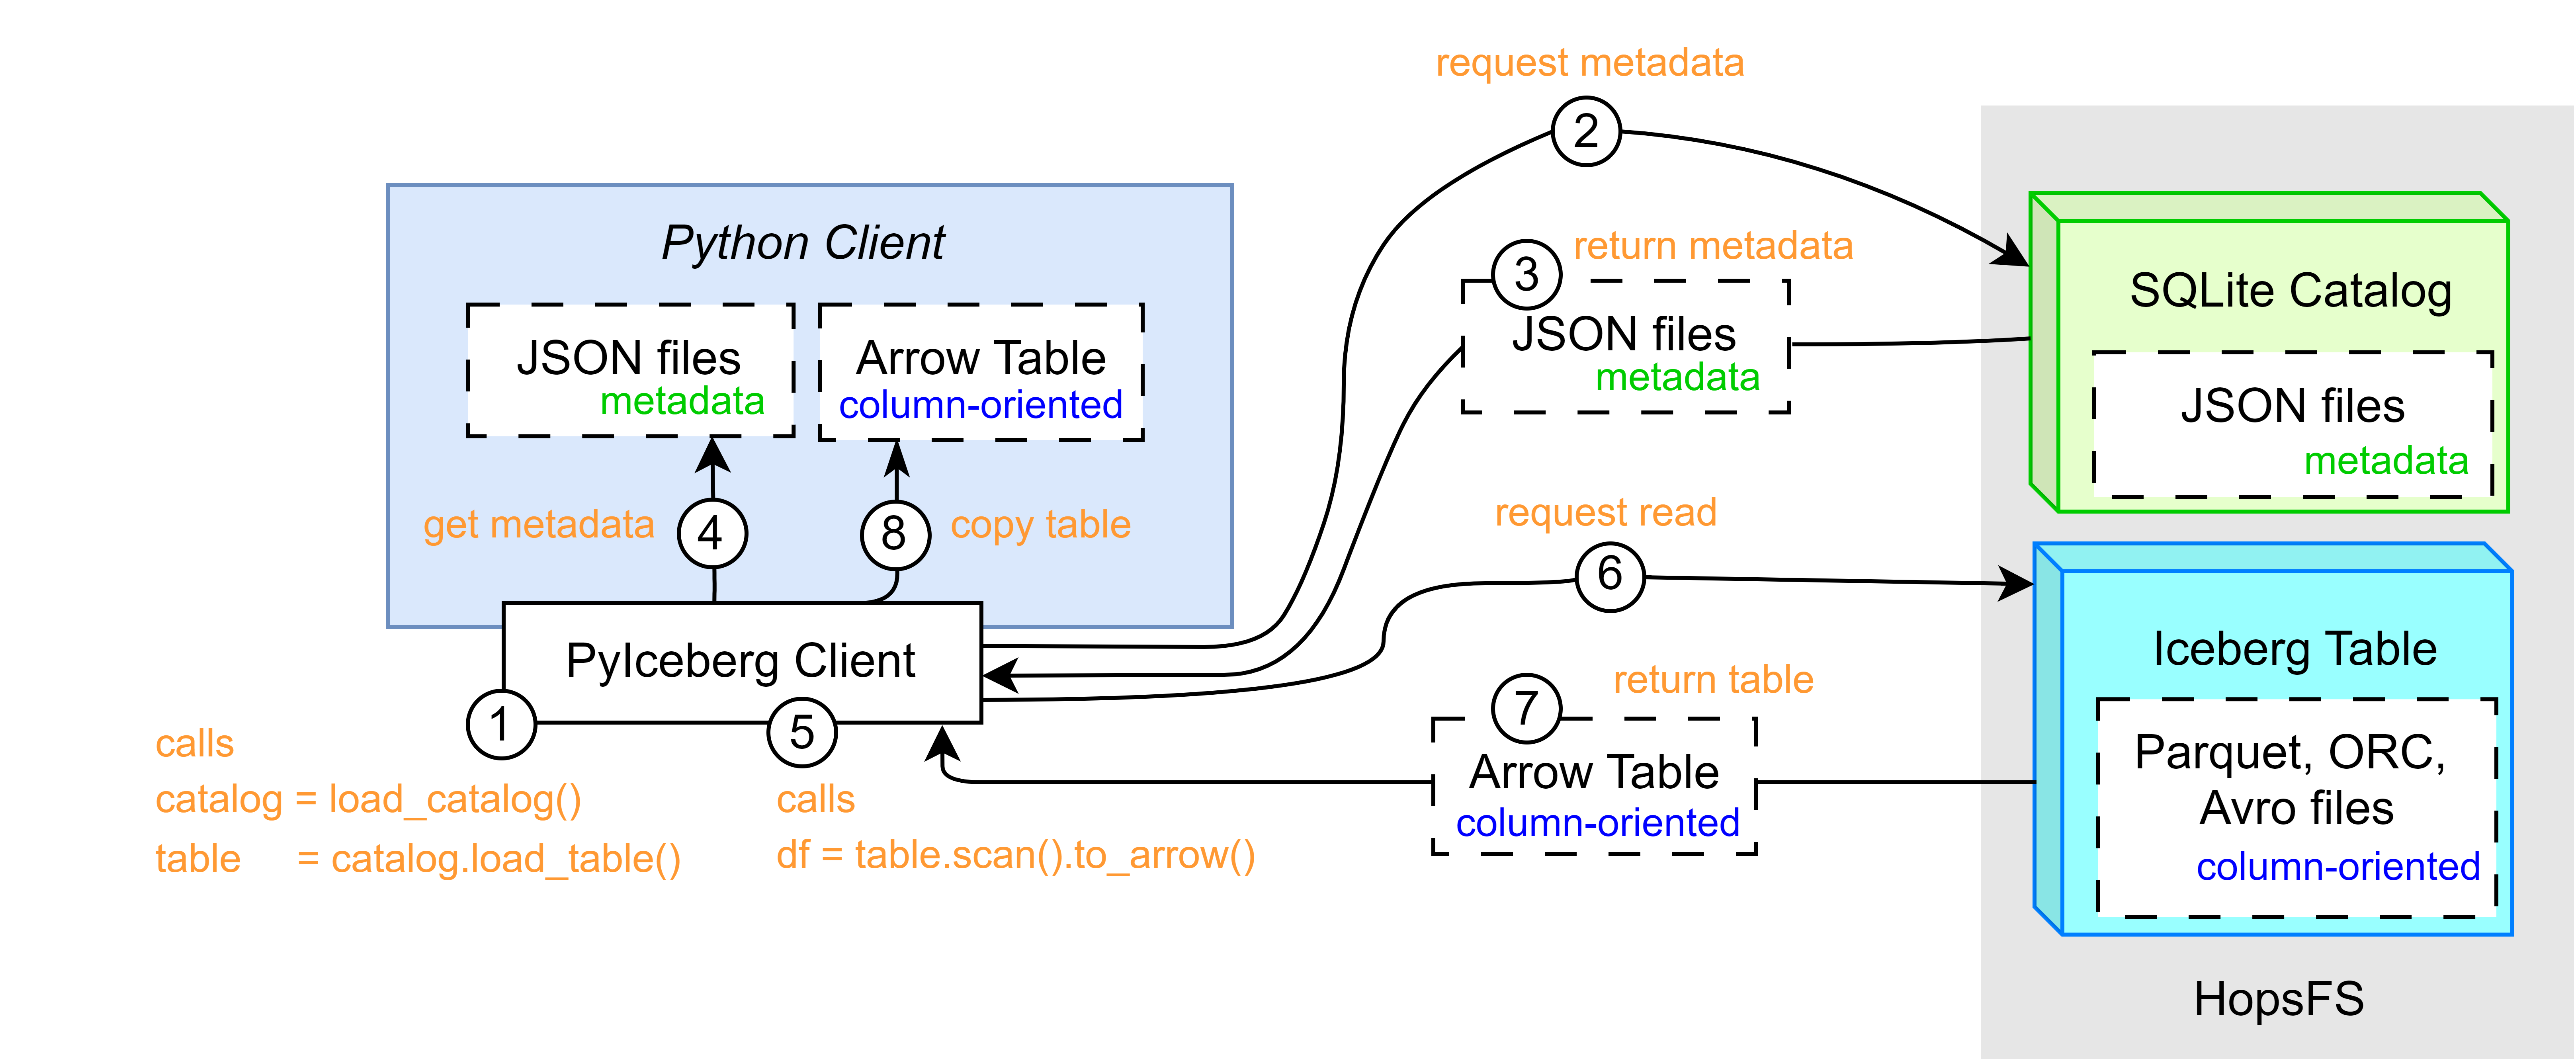
\includegraphics[width=\textwidth]{figures/2-background_and_related_work/iceberg_read.png}
    \end{center}
    \caption[New system - PyIceberg - read process]{PyIceberg library reading an Iceberg Table stored on \gls{HopsFS} and loading it into memory.}
    \label{fig:iceberg_read}
\end{figure}



%%%%% DELTA LAKE WRITE
\subsection{New system - delta-rs - writing}
\label{subsec:back_sys_delta_write}

Figure \ref{fig:delta_write} shows how the delta-rs library writes on a Delta Lake table instanced on top of \gls{HopsFS}. The delta-rs library streamlines the process without passing from a server instance (Spark), removing the middle-tier from the process. In this system, the only file format supported is Parquet, while the other systems supported also ORC and Avro.

\begin{figure}
    \begin{center}
      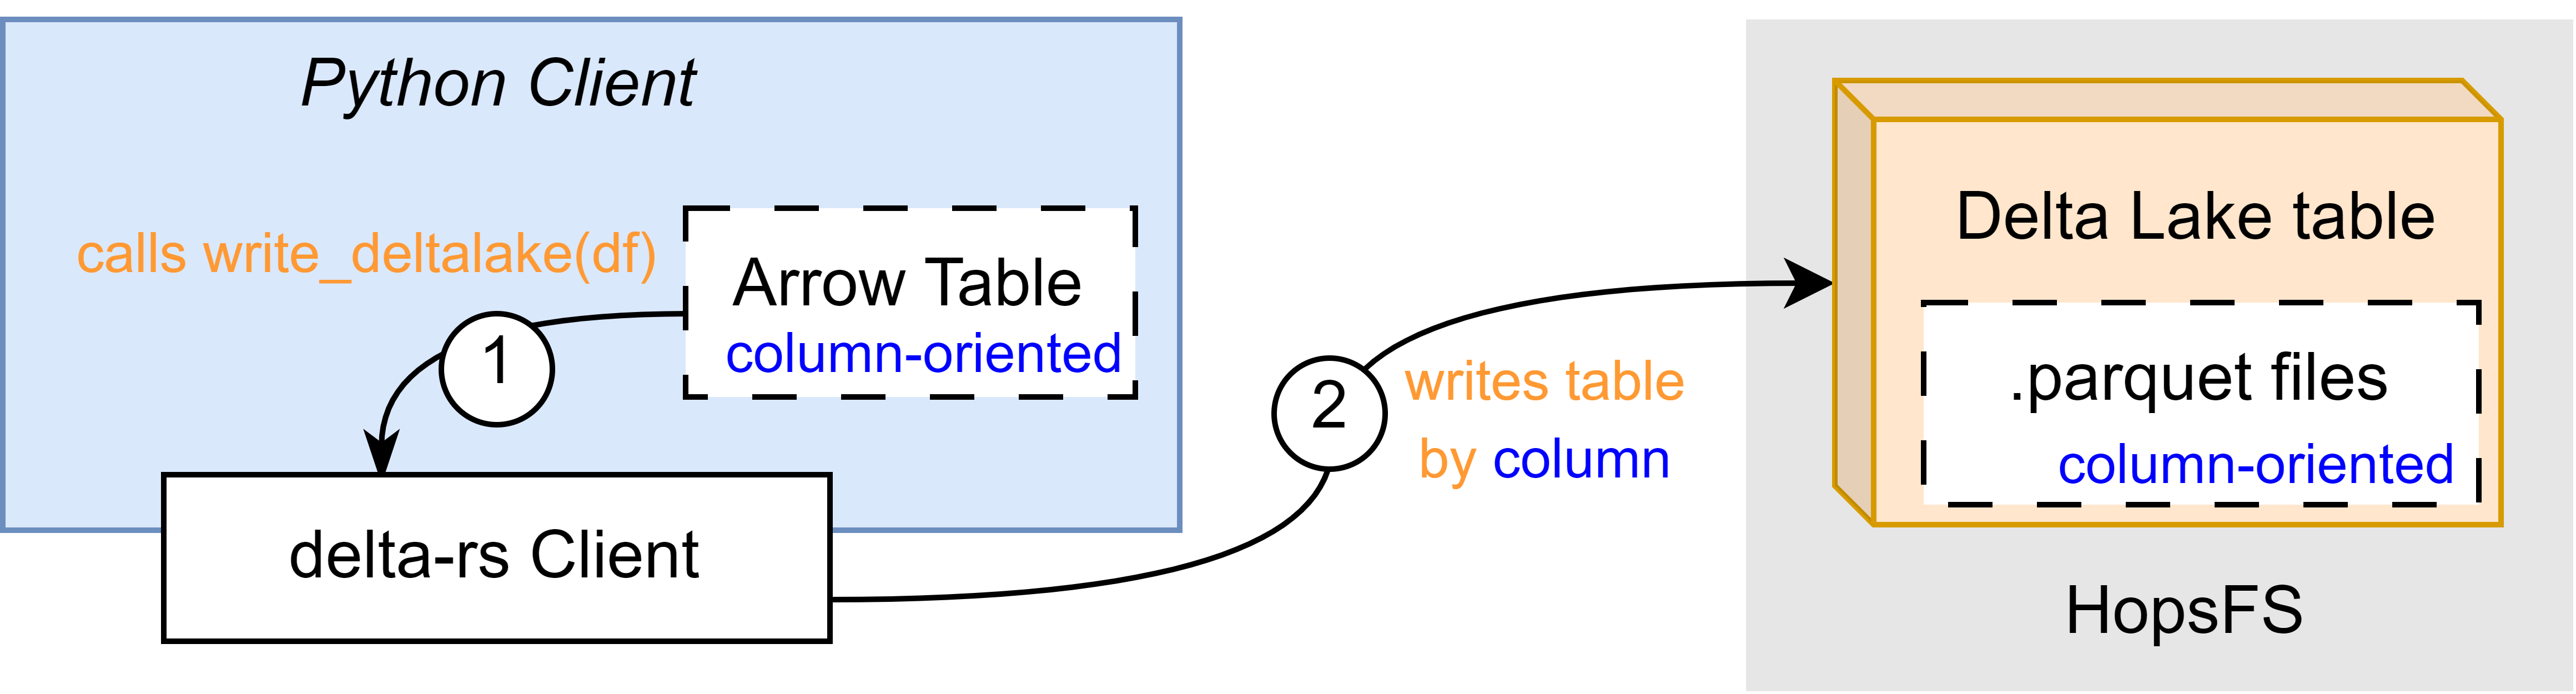
\includegraphics[width=\textwidth]{figures/2-background_and_related_work/delta_write.png}
    \end{center}
    \caption[New system - delta-rs - write process]{Delta-rs library writing an Arrow Table from a Python client to a Delta Lake table stored on \gls{HopsFS}.}
    \label{fig:delta_write}
\end{figure}



%%%%% DELTA LAKE READ
\subsection{New system - delta-rs - reading}
\label{subsec:back_sys_delta_read}

Figure \ref{fig:delta_read} shows how the delta-rs library reads a Delta Lake table instanced on top of \gls{HopsFS}. The delta-rs library streamlines the process without passing from a server instance (Arrow Flight), removing the middle-tier from the process. In this system, the only file format supported is Parquet, while the other systems supported also ORC and Avro.

\begin{figure}
    \begin{center}
      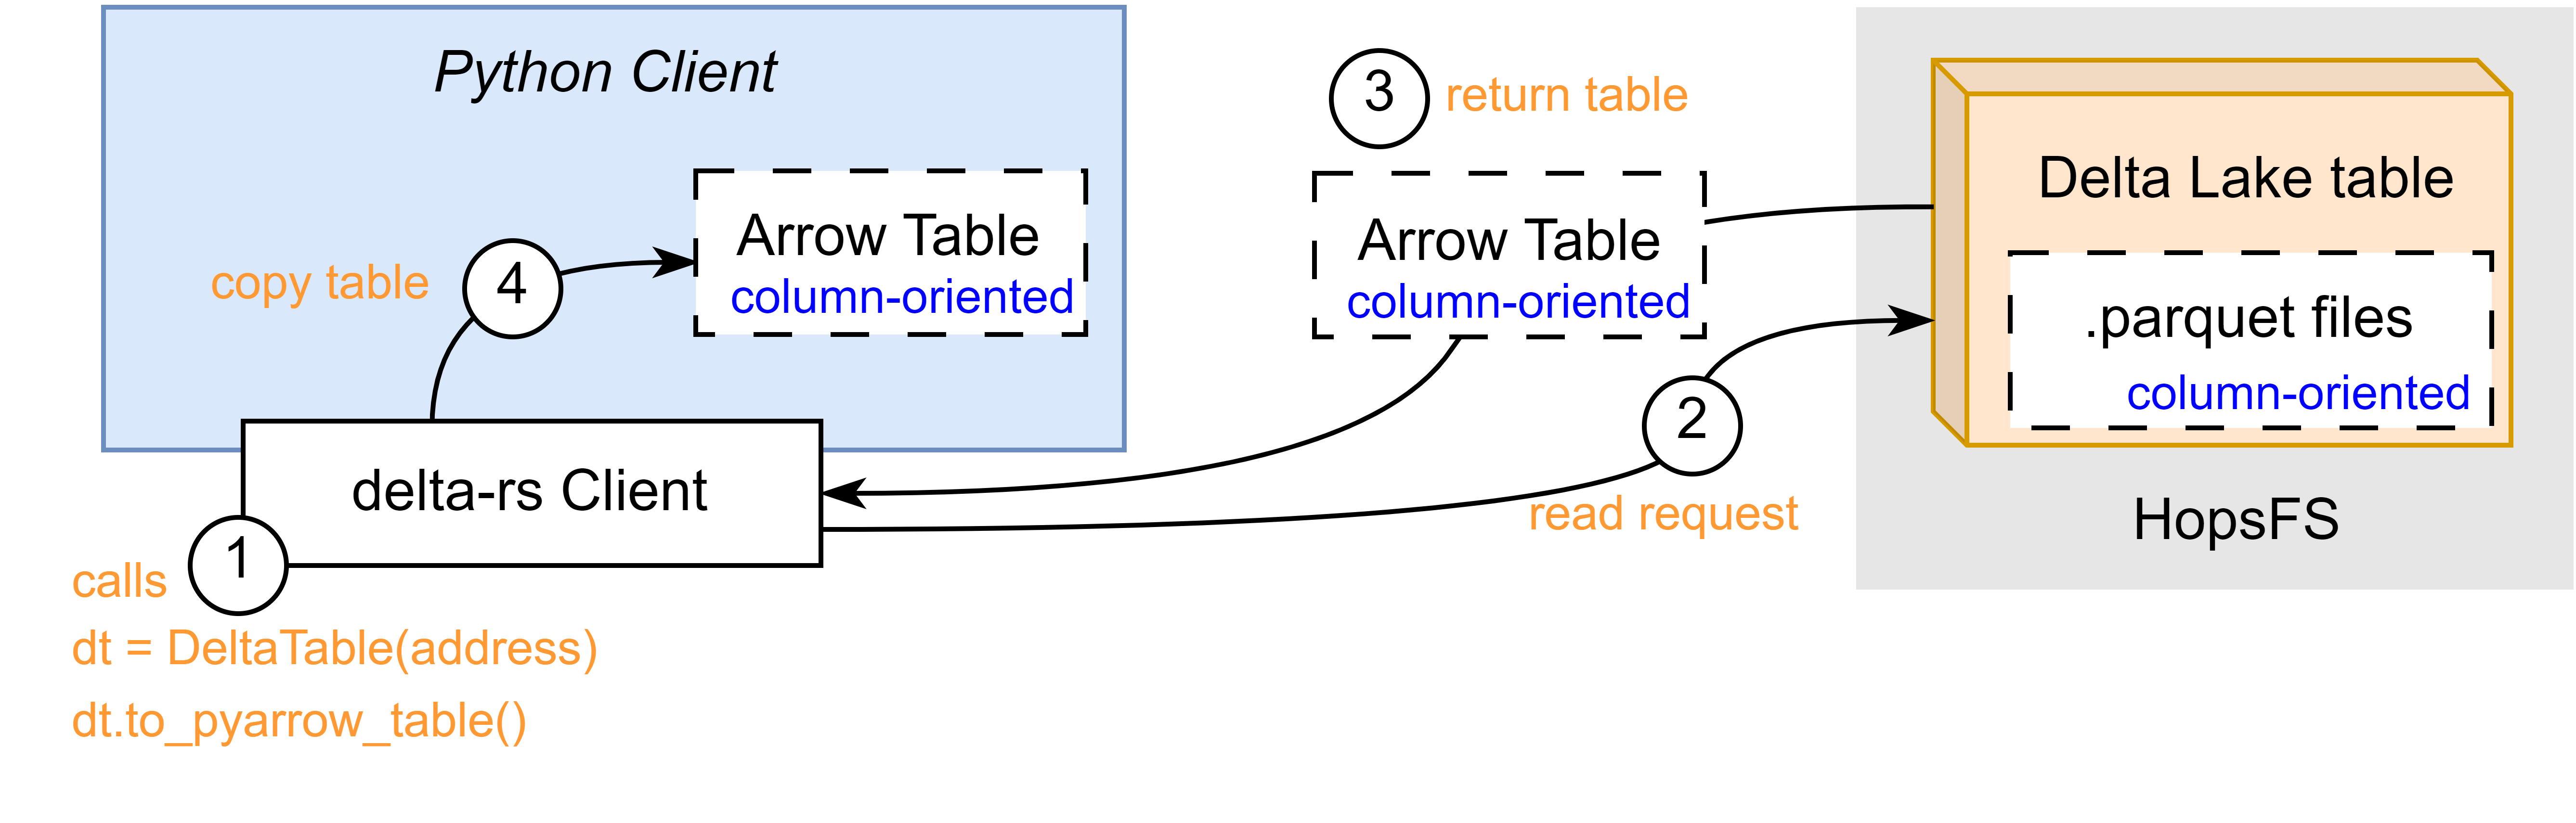
\includegraphics[width=\textwidth]{figures/2-background_and_related_work/delta_read.png}
    \end{center}
    \caption[New system - delta-rs - read process]{Delta-rs library reading a Delta Lake table stored in \gls{HopsFS} and loading it into memory.}
    \label{fig:delta_read}
\end{figure}

\cleardoublepage

\chapter{Method}
    \label{ch:method}
    This chapter defines three methodologies that will be applied sequentially in this project, answering the three \glspl{RQ} defined in Section~\ref{subsec:research_questions}. Section~\ref{sec:system_integration} defines the system integration process that outputs part of \gls{D}3, i.e., the integration detail. This output will enable the Hudi vs. Iceberg system evaluation defined in Section~\ref{sec:system_evaluation_hudi_iceberg}, which will output \gls{D}1, i.e., the results of the experiments. The Iceberg experiment results (\gls{D}1-partial) will enable the Iceberg vs. Delta Lake system evaluation, defined in Section~\ref{sec:system_evaluation_iceberg_delta}, which will output \gls{D}2, i.e.,the results of the comparative experiments. The analysis of \glspl{D}1--2 will be delivered in \gls{D}3, i.e. this comprehensive thesis report.

It has to be noticed that the system evaluation processes, described in Sections \ref{sec:system_evaluation_hudi_iceberg}-\ref{sec:system_evaluation_iceberg_delta}, are inspired by the system evaluation process of a related work \cite{manfrediReducingReadWrite2024}. That related work was hosted by the same company which hosted this thesis work, Hopsworks AB, and it focused on answering \glspl{RQ} on some intent similar to the ones described in Section \ref{subsec:research_questions}. The related work enabled write and read operations on Delta Lake tables stored on \gls{HopsFS}, and investigated performance differences between that system and the current Hopsworks legacy system. Following similar system evaluation processes will not only allow to answer this project's \glspl{RQ}, but will also enable the reader to fairly compare the three technologies investigated in these two thesis works. For the same reason, it easen the comparative process described in Section \ref{sec:system_evaluation_iceberg_delta}, and will make its results more fair and consistent.

\section{System integration}
  \label{sec:system_integration}
  This Section explains the method and principles used for the system integration process, between PyIceberg and \gls{HopsFS}. This Section is divided into three Subsections: Integration process, describing the activities to be conducted to integrate PyIceberg and \gls{HDFS}; Requirements; and Development environment, detailing the tools and resources that will be used during the integration process.


%%%%%  INTEGRATION PROCESS
\subsection{Integration process}
\label{subsec:integration_process}
The integration development process will follow an iterative in Figure \ref{fig:method_code_schema}. This project will require numerous interactions with \gls{HopsFS} maintainers (i.e., the industrial supervisors), since PyIceberg library has to interact with \gls{HopsFS}. This review process creates the need for a feedback loop, allowing the system to fit all the stakeholder requirements, described in Subsection~\ref{subsec:integration_reqs}. This process partially answer \gls{RQ}~1, to which \gls{G}~1-2 are associated, as described in Section~\ref{sec:intro_goals}. The relationships between each process activity and \glspl{G} are here explained:

\begin{enumerate}
    \item \textbf{Set requirements collaboratively}: this activity is key for the completion of \gls{G}~1-2, as it is an initial system analysis, performed together with the industrial supervisors, who are knowledgeable on Hopsworks' infrastructure. This task sets the project requirements and investigates what needs to be integrated at a high-level abstraction.
    \item \textbf{Analyze system and tools}: this activity solves \gls{G}~1 performing low-level code analysis on system and PyIceberg function calls, understanding what needs to be developed to integrate \gls{HopsFS} and PyIceberg. This activity is the first of an iterative loop accounting for the requirements fulfillment.
    \item \textbf{Develop integration}: this activity partially \gls{G}~2, designing and developing a code solution from the information gathered during the analyses above.
    \item \textbf{Test integration}: this activity partially solves \gls{G}~2, verifying the solution validity with integration tests. Failed integration tests or unfulfilled requirements will triggen a new loop iteration. Otherwise, the integretion process will be concluded.
\end{enumerate}

This process will produce a part of \gls{D}~3, which is the code implementation for PyIceberg and \gls{HopsFS} integration, including the consideration about the specific tools selected or discarded.

\begin{figure}[!ht]
    \begin{center}
      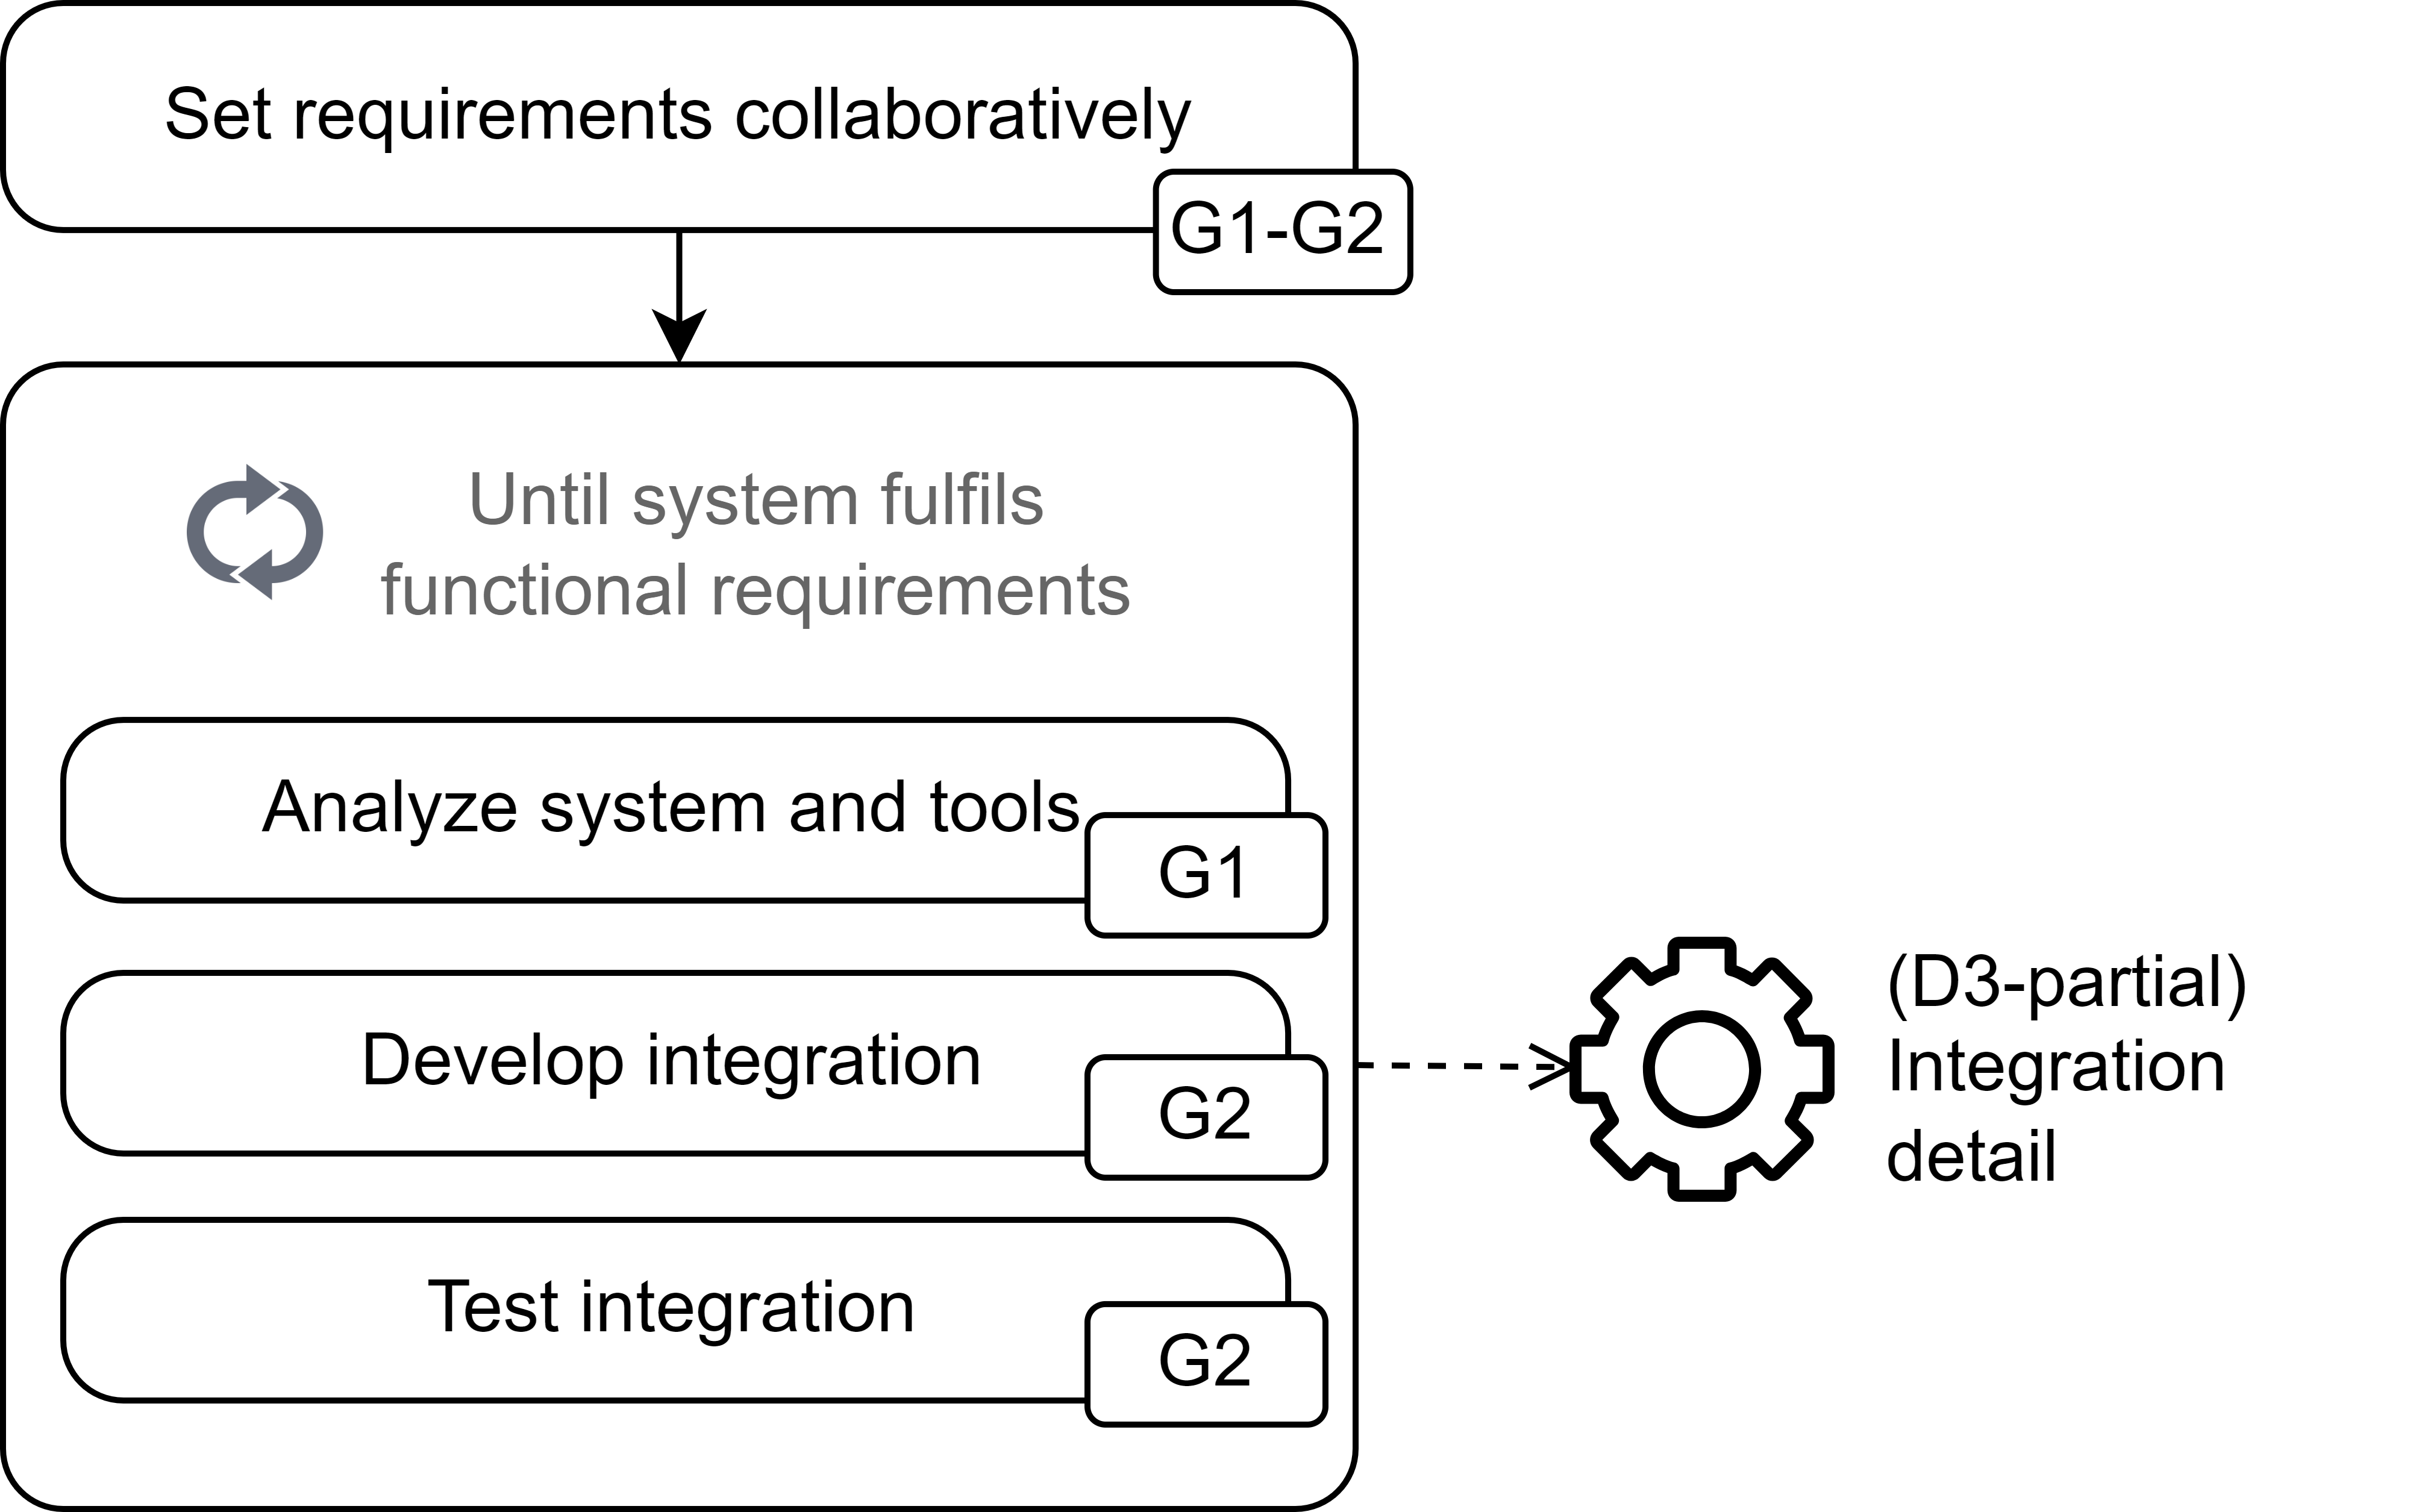
\includegraphics[width=0.8\textwidth]{figures/3-method/method_code.png}
    \caption[System integration process]{Diagram of the system integration process partially answering \gls{RQ}~1. Each activity is associated to specific \glspl{G}. The process produces the integration detail (\gls{D}~3 partial). The loop iterates until the functional requirements, defined in Section~\ref{subsec:integration_reqs}, are fulfilled.}
    \label{fig:method_code_schema}
    \end{center}
\end{figure}


%%%% REQUIREMENTS
\subsection{Requirements}
\label{subsec:integration_reqs}
A series of requirements are defined in agreement with Hopsworks AB, to create a solution that could be later used by the company, in a production environment. The \textbf{functional requirements} are:
\begin{enumerate}
    \item \textbf{Write Iceberg Tables}: the solution should allow to write Iceberg tables on \gls{HopsFS} via the PyIceberg library.
    \item \textbf{Read Iceberg Tables}: the solution should allow to read Iceberg tables on \gls{HopsFS} via the PyIceberg library.
\end{enumerate}
The \textbf{non-functional requirements} are:
\begin{enumerate}
    \item \textbf{Consistent}: the solution should be consistent with the current open-source codebase.
    \item \textbf{Maintainable}: the solution should minimize the need for maintenance and support of the codebase in the future, minimizing changes to open-source code.
    \item \textbf{Scalable}: the solution should handle read or write operations on Iceberg Tables, up to 100 GB, to support small-scale dataset scenarios.
\end{enumerate}


%%%%% DEVELOPMENT ENVIRONMENT
\subsection{Development environment}
The system implementation will be developed using the following technologies:
\begin{itemize}
    \item \textbf{Computing resources}: the system integration will be developed on a \gls{VM} accessed via \gls{SSH} from a computer terminal. Local development will be avoided, due to low reproducibility and complexity of mounting \gls{HopsFS} on a local machine.
    \item \textbf{Code versioning and shared development}: GitHub will be used for versioning and sharing the developed solution.
\end{itemize}


\section{System evaluation - Legacy vs. IcedHops}
  \label{sec:system_evaluation_hudi_iceberg}
  This Section explains the method and principles used for the system evaluation processes, measuring and comparing the performance (latency, in seconds, and throughput, in rows/second) of reading and writing Hudi and Iceberg tables on \gls{HopsFS}. Those operations are conducted respectively on the current legacy system and on the PyIceberg-based system, integrated in this thesis work.

\subsection{Evaluation process - RQ2}
\label{subsec:eval_process_hudi_iceberg}
This evaluation process will follow a sequential approach described in Figure~\ref{fig:method_experiments}. Each step of this process is related to one of the \glspl{G}3--6 associated with the \gls{RQ}2 in Section \ref{sec:intro_goals}, to which this process answers. The relationships between each process activity and \glspl{G} are here explained:
\begin{enumerate}
    \item \textbf{Design experiments}: this activity maps perfectly to \gls{G}3, designing the experiments that will be conducted to evaluate the performance difference in performance between the current legacy access to Apache Hudi compared to the PyIceberg library-based access to Icbeerg Tables in \gls{HopsFS}. 
    \item \textbf{Perform experiments}: this activity maps perfectly to \gls{G}4, using the integration detail (\gls{D}3-partial) to develop and conduct the designed experiments on the analyzed systems. Here, data is collected as latency, expressed in seconds.
    \item \textbf{Transform data according to metrics}: this activity is requisite to fulfill \gls{G}5, and \gls{G}8 of \gls{RQ}3. The activity is conducted because throughput is not directly measured, but it is computed from latency following the formula here below:
    \[ Throughput \; (rows/second) = \frac{Number \; of \; rows \; (rows)}{Latency \;(seconds)}\]
    \item \textbf{Visualize results}: this activity maps perfectly to \gls{G}5, visualizing the experiments' result according latency, measured in seconds, and throughput, measured in rows/second. This activity also generates \gls{D}1, the experiment results complemented with tables and histograms, presented in Chapter \ref{ch:results_and_analysis}.
    \item \textbf{Analyze results}: this activity maps perfectly to \gls{G}6, analyzing and interpreting the results delivered in \gls{D}1. This activity contributes to \gls{D}3, generating the analysis of experimental results, presented in Chapter \ref{ch:results_and_analysis}.
\end{enumerate}
\begin{figure}[!ht]
    \begin{center}
    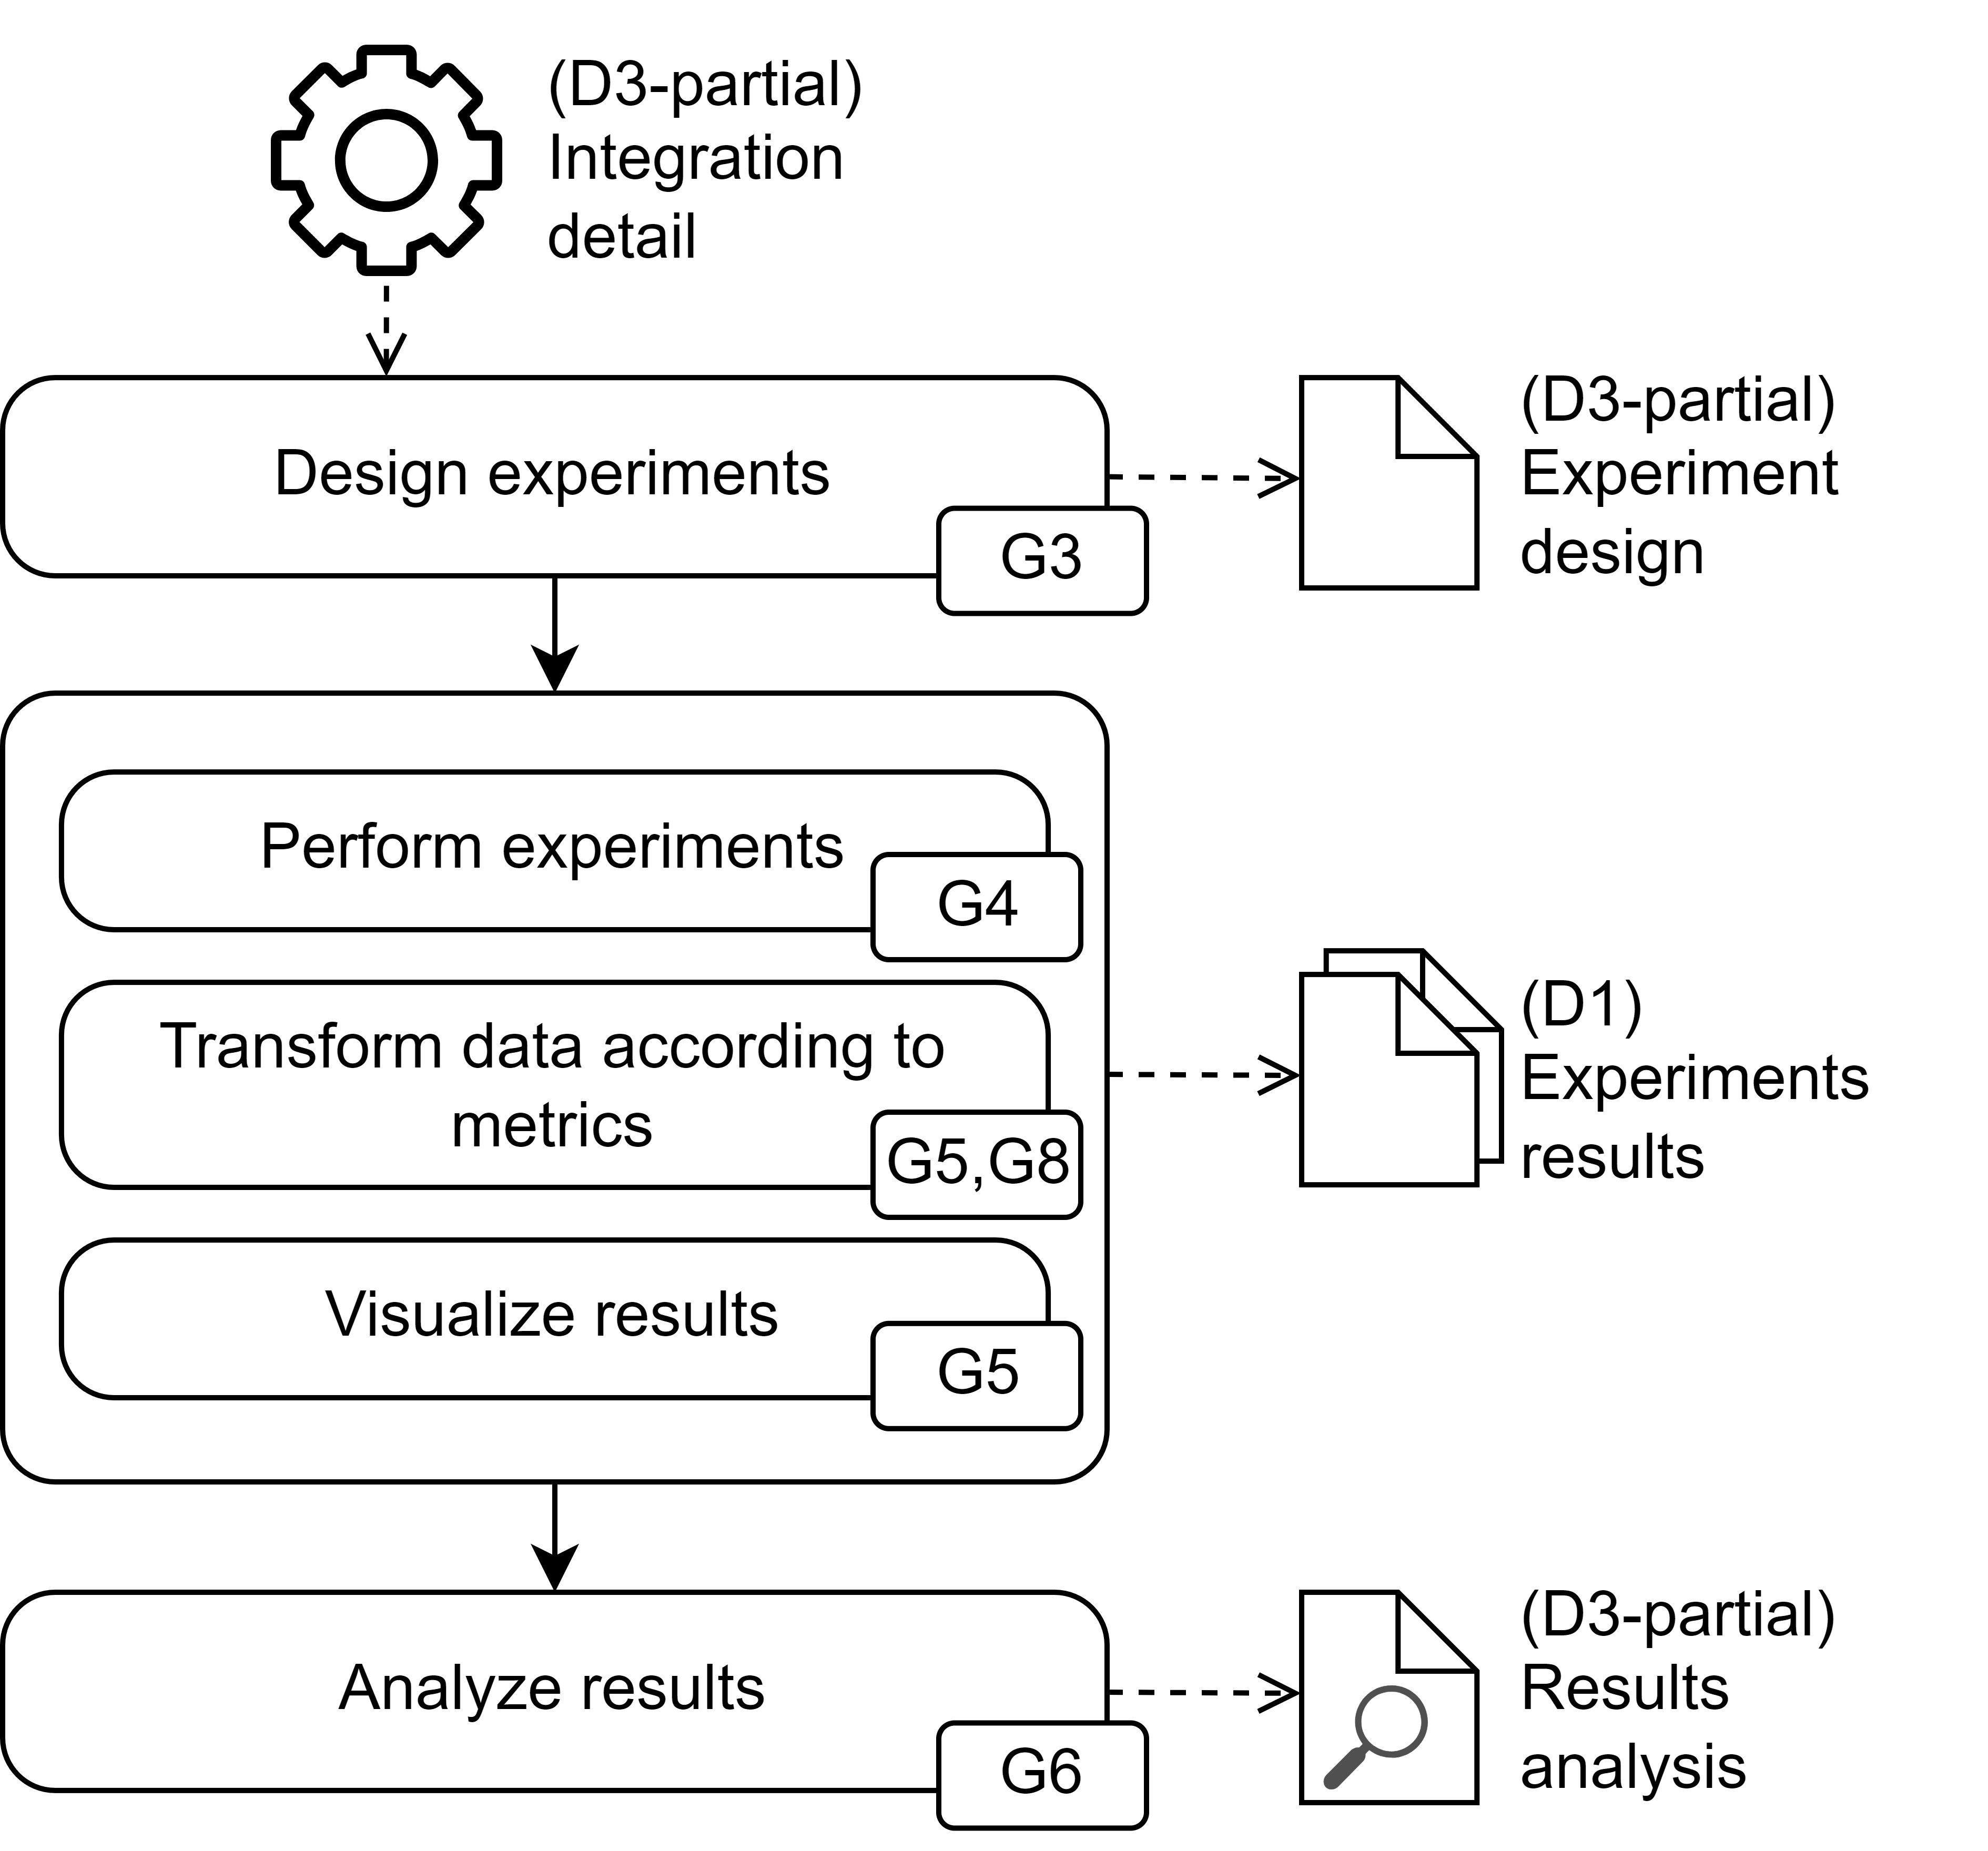
\includegraphics[width=0.7\textwidth]{figures/3-method/method_exp.png}
    \caption[System evaluation process - Hudi vs. Iceberg]{Diagram of the system evaluation process answering \gls{RQ}2. Each activity is associated to specific \gls{G}. The process produces two \glspl{D}, the experiments results (\gls{D}1) and a results analysis (\gls{D}3-partial).}
    \label{fig:method_experiments}
    \end{center}
\end{figure}


%%%% INDUSTRIAL USE CASE
\subsection{Industrial use case}
\label{subsec:method_use_case}

Several choices must be made for a system evaluation: which data will be used, which environment will run the experiments, and which metrics will be used to evaluate the system. Those choices depends on the scenarios for which the system is created. Thus, this Subsection describes the typical use case for this system. Follwing, the other Subsections describe which were the decision taken accordingly. While conducting their research in Hopsworks, the author outlined a typical industrial use case for the Hopsworks feature store, by reading internal documentation and discussing with several employees on their customer needs and trends. The use case is described by:
\begin{itemize}  
  \item \textbf{Table size}: most of the Hospworks' customers' workloads were limited (from 1M to 100M rows), with only few clients needing support for massive workloads (more than 1B rows). Thus, this project opted to improve performance for the smaller workloads (from 100k to 100M rows). The datatset selected are presented in Section~\ref{subsec:experimental_data}.
  \item \textbf{Type of data}: the Hopsworks feature store works only with structured data (e.g., numbers, strings), thus experiment design and selected datasets embody this scenario.
  \item \textbf{Rows over storage size}: In the experimental part of this thesis, in order to have a reliable unit measure for table size, the number of rows will be over the storage size (bytes). Perhaps, in the structured data domain of this use case, storage size (bytes) is neither linked to a table structure nor to a storage structure, arguably making this unit measure not reliable (i.e, table with a lot of rows and few columns, and a table with few ros and a lot of columns occupies the same memory).
  \item \textbf{Client configuration}: the client configuration is modeled to reflect typical customers' clients' computational and storage capabilities. Thus, the configuration are limited between one and eight \gls{CPU} cores, \gls{RAM} just sufficient for system needs and common \gls{SSD} storages. The experimental environment is further detailed in Section~\ref{subsec:experimental_env}.
\end{itemize}



%%%% EXPERIMENTAL DATA %%%%
\subsection{Experimental data}
\label{subsec:experimental_data}

The datasets that will be used to perform read and write experiments come from \glsentryshort{TPC}-H benchmark suite~\footnote{Benchmark suite website available at \url{https://www.tpc.org/tpch/}}. \glsentryshort{TPC}-H is a decision support benchmark by \gls{TPC}, that consists in a collection of business-oriented queries in specific industry sectors \cite{transactionprocessingperformancecounciltpcTPCH_v301pdf1993}, which became the de-facto standard for experiments on data storage system. Perhaps, it has been used in related studies \cite{raasveldtDuckDBEmbeddableAnalytical2019,behmPhotonFastQuery2022,manfrediReducingReadWrite2024}. 

The \glsentryshort{TPC}-H benchmark contains eight tables, and any part of the data can be generated via the \glsentryshort{TPC}-H data generation tool~\footnote{Available at \url{https://www.tpc.org/tpc_documents_current_versions/current_specifications5.asp}}. The two tables that will be used are the SUPPLIER and the LINEITEM, respectively, the smallest (10k rows) and largest (60M rows) tables. The size (number of rows) of a table depends on the \gls{SF}, that can be varied to progressivly change in the table size. The SUPPLIER table has seven columns, while the LINEITEM table has sixteen. This difference influences the average size of memory each row occupies. Below for each table their columns are listed, specifying which data type they store.
\begin{itemize}
  \item SUPPLIER
  \begin{itemize}
    \item S\_SUPPKEY : identifier
    \item S\_NAME : fixed text, size 25
    \item S\_ADDRESS : variable text, size 40
    \item S\_NATIONKEY : identifier
    \item S\_PHONE : fixed text, size 15
    \item S\_ACCTBAL : decimal
    \item S\_COMMENT : variable text, size 101
  \end{itemize}
  \item LINEITEM
  \begin{itemize}
    \item L\_ORDERKEY : identifier
    \item L\_PARTKEY : identifier
    \item L\_SUPPKEY : identifier
    \item L\_LINENUMBER : integer
    \item L\_QUANTITY : decimal
    \item L\_EXTENDEDPRICE : decimal
    \item L\_DISCOUNT : decimal
    \item L\_TAX : decimal
    \item L\_RETURNFLAG : fixed text, size 1
    \item L\_LINESTATUS : fixed text, size 1
    \item L\_SHIPDATE : date
    \item L\_COMMITDATE : date
    \item L\_RECEIPTDATE : date
    \item L\_SHIPINSTRUCT : fixed text, size 25
    \item L\_SHIPMODE : fixed text, size 10
    \item L\_COMMENT : variable text, size 44
  \end{itemize} 
\end{itemize}

Considering the different structure of the two tables used (i.e., number of columns and data types) comparison across different tables cannot be done using the the selected metrics, i.e., latency (seconds) and throughput(rows/second). For this reason, the system evaluation will only consider same tables on different configuration. This project used five table variations to benchmark the system integration. \gls{SF} was varied to obtain a table at each significant order of magnitude from 10k to 60M rows. These are the tables:
\begin{enumerate}
    \item \textit{supplier\_sf1}: size = 10000 rows
    \item \textit{supplier\_sf10}: size = 100000 rows
    \item \textit{supplier\_sf100}: size = 1000000 rows
    \item \textit{lineitem\_sf1}: size = 6000000 rows
    \item \textit{lineitem\_sf10}: size = 60000000 rows
\end{enumerate}

Lastly, despite no information are given about the row and storage size (bytes) ratio, in accordance to Section \ref{subsec:method_use_case}, this Section presentes comprehensive information on the data, including how to retrieve it and how it is composed. These gives to the reader the ability of calculating the storage occupancy of each table, depending on their prefered unit of measure.



%%%% EXPERIMENTAL DESIGN
\subsection{Experimental design}
\label{subsec:experimental_design}

The experiments aim to highlight the differences between the current legacy system and the the newly implemented system based on the PyIceberg library. Two experimental pipelines were designed to isolate the performance of those two systems:
\begin{enumerate}
  \item \textbf{Legacy pipeline}: is the current Hopsworks feature store which stores data in Hudi tables. This system uses a pipeline based on Kafka, and Spark to write data on the Hudi tables, saved on \gls{HopsFS}. The pipeline uses a Spark alternative, DuckDB, and Arrow Flight to read data. This is described in Sections \ref{subsec:back_sys_hudi_write}-\ref{subsec:back_sys_hudi_read}.
  \item \textbf{PyIceberg - \glsentryshort{HopsFS}}: is the system implemented in Chapter \ref{ch:implementation}, which stores data in Iceberg Tables. This systems uses a pipeline based on PyIceberg, SQLite, and Arrow Flight to both write to and read from the Iceberg tables, saved on \gls{HopsFS}. This is described in Sections \ref{subsec:back_sys_iceberg_write}-\ref{subsec:back_sys_iceberg_read}.
\end{enumerate}

The experiments will verify how the performance will change based on different \gls{CPU} resources provided: one, two, four, and eight cores, according to the typical Hopsworks use case (Section \ref{subsec:method_use_case}). Each time, the experimental environment will be modified, creating a new Jupyter server where the host the experiments. The data used for experiments, as described in Section \ref{subsec:experimental_data}, will come from two different tables, modified according to a \gls{SF}, for a total of five times for each table. For the writing experiments conducted on the legacy system, different parts of the whole writing process will be measured, to verify how different parts of the legacy system will scale in the different environments described above. Those two parts are the upload and the materialization, which are explained in Section \ref{subsec:back_sys_hudi_write}. This will also help defining whether and what part of the legacy pipeline is a bottleneck.

In conclusion, the experiments conducted will be a total of two (pipelines) times four (\gls{CPU} configurations) times five (tables) times two (read and write operations), thus eighty experiments, performed each fifty times, to ensure statistical significancy to the results.



%%%% EXPERIMENTAL ENVIRONMENT
\subsection{Experimental environment}
\label{subsec:experimental_env}

The experimental environment consists of a physical machine in Hopsworks AB' offices, virtualized to enable remote shared development. The \gls{CPU} details of the machine are present in Listing \ref{lst:cpu_snurran}, noting that only eight cores at maximum were dedicated during the experiments. The machine mounts about 5.4 TBs of \gls{SSD} memory, allowing for fast read and write speed, respectively 2.7 GB/s, and 1.9 GB/s (measured with a simple \textit{dd} bash command). The experimental environment will be set up with a Jupyter Server of different CPU cores, depending on the experiment. The Jupyter server is allocated by default with 2048MB, which will be adjusted during the experiments, according to the needs (see Section \ref{subsec:resources_usage}).

Notica that, despite this experimental environment is virtualized in isolation, it runs on shared resources, thus experiments result might vary depending on the machine's load. To mitigate this, all experiments will be run when the machine load is low (less than 50\% of \gls{CPU} and \gls{RAM} usage).

\begin{lstlisting}[language=bash, caption={[Experimental environment details]Output of a \textit{lscpu} bash command on the machine.}, label={lst:cpu_snurran}, frame=tb, basicstyle=\small]
Architecture:            x86_64
  CPU op-mode(s):        32-bit, 64-bit
  Address sizes:         48 bits physical, 
                         48 bits virtual
  Byte Order:            Little Endian
CPU(s):                  32
  On-line CPU(s) list:   0-31
Vendor ID:               AuthenticAMD
  Model name:            AMD Ryzen Threadripper 
                         PRO 5955WX 16-Cores
    CPU family:          25
    Model:               8
    Thread(s) per core:  2
    Core(s) per socket:  16
    Socket(s):           1
    Stepping:            2
    Frequency boost:     enabled
    CPU max MHz:         7031.2500
    CPU min MHz:         1800.0000
    BogoMIPS:            7985.56
Virtualization features: 
  Virtualization:        AMD-V
Caches (sum of all):     
  L1d:                   512 KiB (16 instances)
  L1i:                   512 KiB (16 instances)
  L2:                    8 MiB (16 instances)
  L3:                    64 MiB (2 instances)
\end{lstlisting}



%%%% EVALUATION FRAMEWORK
\subsection{Evaluation framework}
\label{subsec:method_eval_framework_hudi_iceberg}

The system evaluation framework will evaluate the different system on three key aspects:
\begin{enumerate}
    \item \textbf{Functional requirements}: will be measured by verifying the success or failure of running an experiment. This will not happen by design, since the system integration phase stops only when all functional requirements are met. Those are escribed in Section \ref{subsec:integration_reqs}:
    \item \textbf{Non-functional requirements}: Consistency and maintainability are mainly addressed during integration, while scalability is measured during the system evaluation experiments. The metric used for measuring this requirement is the throughput, as defined in \gls{RQ}1.
    \item \textbf{How does the legacy pipeline compare to the PyIceberg pipeline?} this question answers directly \gls{RQ}2, measuring the throughput of the pipelines defined in Section \ref{subsec:experimental_design}. Results are then compared using a visual approach.
\end{enumerate} 



%%%% RELIABILITY AND VALIDITY
\subsection{Reliability and validity}
\label{subsec:method_reliability_validity}

Experiments result are significant according to their reliability and validity. Each experiment will be performed fifty times to ensure the reliability of the its results on the system performance. This number was agreed to balance the results' consistency and resource efficiency (i.e., time and computing resources), as described in Section \ref{sec:intro_ethics_and_sustainability}. Secondly, due to the complex nature of the pipelines used, the data distribution of results might vary from one experiment to the other. Thus, a bootstrapping technique will be employed to restore the validity of the data collected. Data will be resampled with substitutions a thousand times, then for each experiment an average measure, altogether with a confidence interval.

\section{System evaluation - IcedHops vs. Delta Lake}
  \label{sec:system_evaluation_iceberg_delta}
  This Section firstly explains the steps of this system evaluation processes, aimed at measuring and comparing the performance (latency, in seconds, and throughput, in rows/second) of reading and writing Iceberg and Delta Lake tables on \gls{HopsFS}. Those experiments will be conducted respectively on the PyIceberg-based system, integrated in this thesis work, and on the delta-rs-based system, implemented in a related work \cite{manfrediReducingReadWrite2024}. Then, it presents the evaluation framework used by in this process.



%%%% EVALUATION PROCESS
\subsection{Evaluation process - RQ3}
\label{subsec:eval_process_iceberg_delta}
This evaluation process will follow a sequential approach described in Figure~\ref{fig:method_comparison}. Each step of this process is related to one of the \glspl{G}7--9 associated with the \gls{RQ}3 in Section \ref{sec:intro_goals}. The relationships between each process activity and \glspl{G} are here explained:
\begin{enumerate}
    \item \textbf{Analyze related work results}: this activity maps perfectly to \gls{G}7, analyzing the results coming from the related work taken as input by this process.
    \item \textbf{Visualize results}: this activity maps perfectly to \gls{G}8. It takes as input also PyIceberg experiments results (\gls{D}1-partial), visualizing thus the experiments' result according to latency and throughput. This activity generates \gls{D}2, the comparative experiments results complemented with tables and histograms, presented in Chapter \ref{ch:results_and_analysis}.
    \item \textbf{Analyze results}: this activity maps perfectly to \gls{G}9, analyzing and interpreting the results delivered in \gls{D}2. This activity contributes to \gls{D}3, generating the comparative analysis of the experiment results, presented in Chapter \ref{ch:results_and_analysis}.
\end{enumerate}
\begin{figure}[!ht]
    \begin{center}
    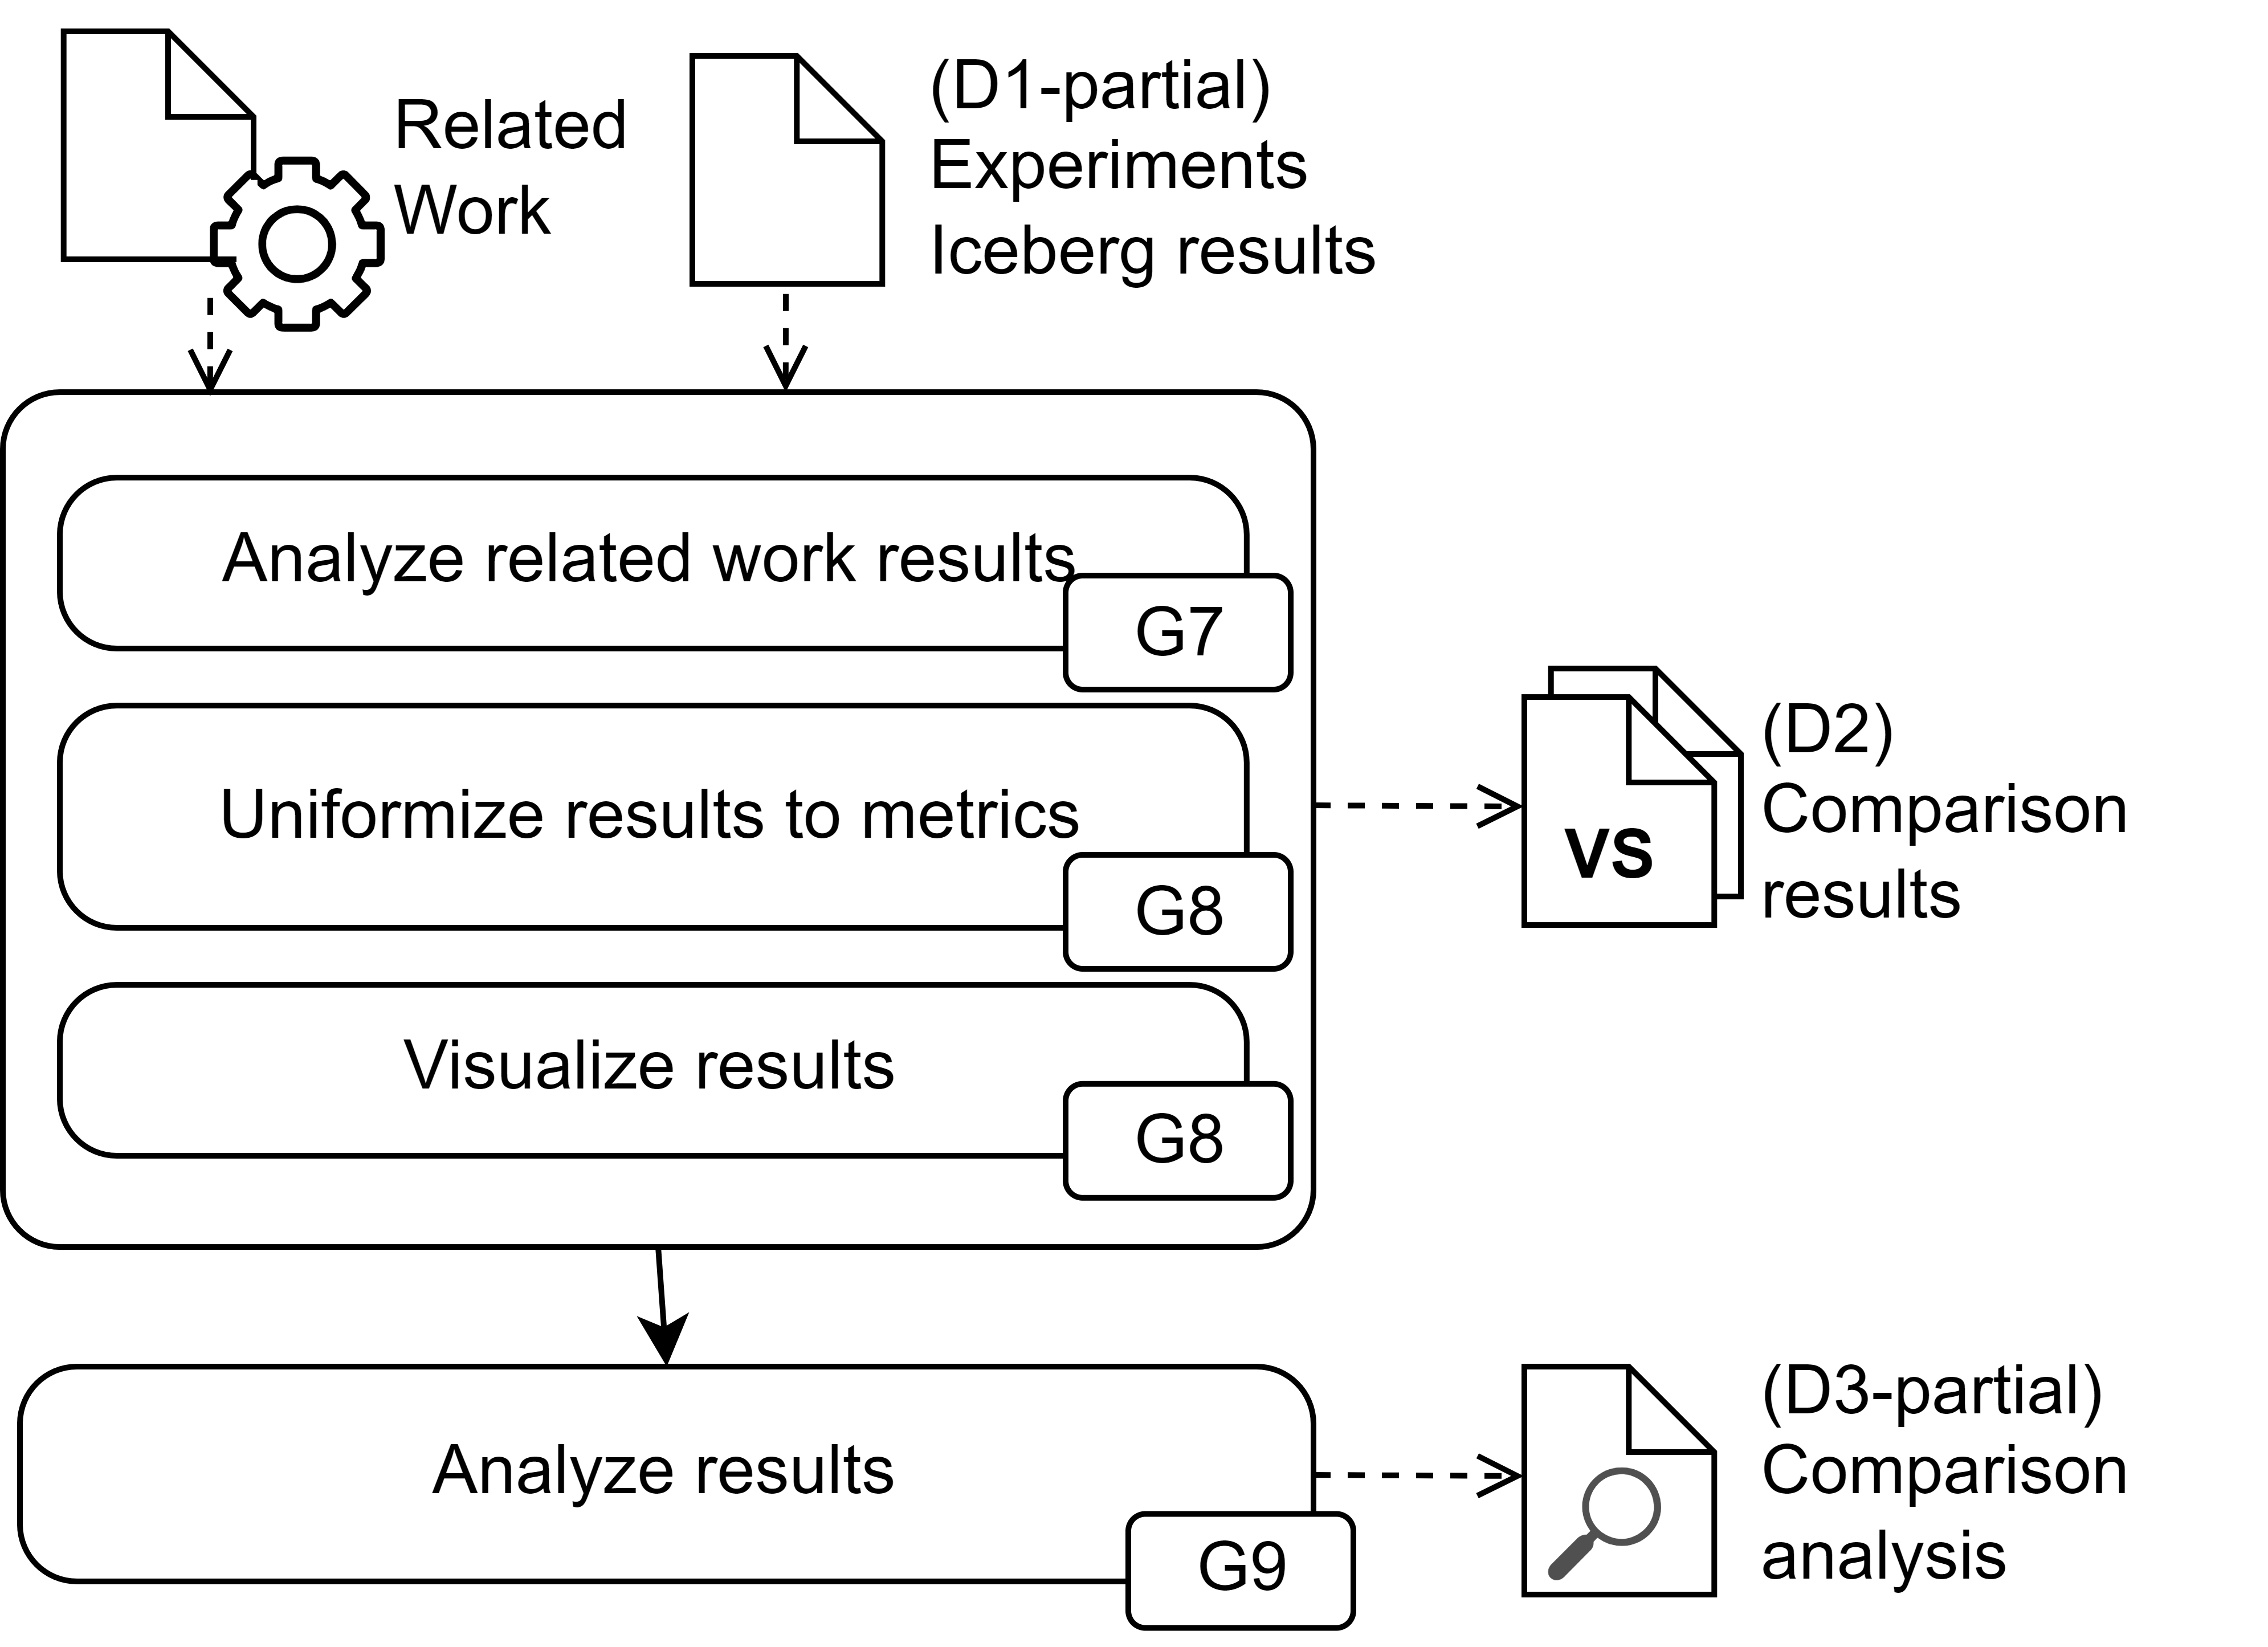
\includegraphics[width=0.7\textwidth]{figures/3-method/method_comp.png}
    \caption[System evaluation process - PyIceberg vs. delta-rs]{Diagram of the system evaluation process answering \gls{RQ}3. Each activity is associated to specific \gls{G}. The process produces two \glspl{D}, the comparative expertiments results (\gls{D}2) and a comparative results analysis (\gls{D}3-partial).}
    \label{fig:method_comparison}
    \end{center}
\end{figure}



%%%% EVALUATION FRAMEWORK
\subsection{Evaluation framework}
\label{subsec:method_eval_framework_iceberg_delta}

This system evaluation framework is similar to the system evaluation framework described in Section \ref{subsec:method_eval_framework_hudi_iceberg}, but will not focus on functional requirements, as they will be already assessed in previous Section, for PyIceberg, and they have been already assessed in the related work, for delta-rs. Thus, this evaluation framework will evaluate the different system on two key aspects:
\begin{enumerate}
    \item \textbf{Non-functional requirements}: Consistency and maintainability are mainly addressed during integration, while scalability is measured during the system evaluation experiments. The metric used for measuring this requirement is the throughput, as defined in \gls{RQ}2.
    \item \textbf{How does the PyIceberg pipeline compare to the delta-rs pipeline?} this question answers directly \gls{RQ}3, measuring the throughput of the PyIceberg pipeline defined in Section \ref{subsec:experimental_design} and the delta-rs pipeline \cite{manfrediReducingReadWrite2024}. Results are then compared using a visual approach.
\end{enumerate}




\cleardoublepage

\chapter{Implementation}
    \label{ch:implementation}
    This Chapter follows first the system integration process, defined in Section \ref{sec:system_integration}, describing which integration choices were taken, which components were selected and their usage. Thus it explains how was conducted the experimental part of this thesis, presented in Section \ref{sec:system_evaluation_hudi_iceberg}.

\section{Integration design and usage}
    \label{sec:integration_design_and_usage}
    The first step of the system integration process consisted of analyzing the Hopsworks system and the PyIceberg tools, as described in Section \ref{sec:system_integration}. This permitted to identify which parts had to be integrated to satisfy the requirements, thus to be able to read and write on Iceberg Table hosted on \gls{HopsFS}, via the PyIceberg library. This step outlined the need of a catalog, a query engine, and a FileIO. While the formers are fundamental components of any Data lakehouse architecture explained in Section \ref{subsec:datalakehouse_architecture}, the latter is a pluggable module for performing \gls{CRUD} operations on files, specifically required by PyIceberg.

PyIceberg, being a rather recently developed library, does not provides yet all the features integrations of older Iceberg libraries \cite{iceberg_tech_docs}, such the Java \gls{API}. In addition, despite \gls{HopsFS} expose the same methods of \gls{HDFS}, the environment where HopsFS was mounted, described in Section \ref{subsec:experimental_env}, did not allow to use some catalogs. Sections \ref{subsec:integration_catalog_choice}-\ref{subsec:integration_engine_choice} describe the choices taken for both catalog (SQL Catalog) and query engine (DuckDB), describing the reason behind those choices and the problem encountered~\footnote{Code available at: https://github.com/SebastianoMeneghin/apache-iceberg-as-offline-feature-store}. Regarding the FileIO, since there was a single compatible option (PyArrowFileIO), this component could not be subject of any design comparison. Lastly, Section \ref{subsec:integration_usage} describe how instanciate the integrated system, and how to perform operations over it.

\subsection{Catalog choice}
\label{subsec:integration_catalog_choice}
At time of development, the available catalogs were:
\begin{itemize}
    \item \textbf{REST}: it is supported by \gls{HopsFS}. However, since this would have need to develop the interface from scratch, thus was discarded as not fulfilling the maintainability not-functional requirement, described in Section \ref{subsec:integration_reqs}.
    \item \textbf{\gls{AWS} Glue}: it is supported by \gls{HDFS}, but it did not pass the integration test with \gls{HopsFS}, thus was discared. Additionally, since it is a proprietary solution of \gls{AWS}, this would have lowered the reproducibility of the experiments later conducted, due to the additional costs of this solution.
    \item \textbf{\gls{AWS} DynamoDB}: it is supported by \gls{HopsFS}. Was however discarded, for the same reproducibility reason explained above.
    \item \textbf{\gls{HMS}}: it is supported by \gls{HopsFS}. \gls{HMS} is however a complex tool, developed to be tightly integrated with MapReduce and Spark environment, and perhaps perform its best in large-scale data scenarios. This was discared since not matching with purpose of avoiding Spark and its environment, and the industrial use case described in Section \ref{subsec:method_use_case}. Furthermore, this did not fulfill the maintainability not-functional requirement.
    \item \textbf{SQL Catalog}: it is supported by \gls{HopsFS}, and it could be instanciated on a SQLite database supported by PyIceberg. This was the choice for the system integration, as it is an open-source catalog, the most light-weight option among the alternatives, and needs few lines of code to be used, fulfilling both the not-functional and the functional requirements. This solution suits perfectly small-scale scenarios such this thesis' use case, but it does not fit a large-scale scenario. Furthemore, the specific SQLite database is not built for concurrency.
\end{itemize}

\subsection{Query engine choice}
\label{subsec:integration_engine_choice}
In the choice of the query engine, all the candidates are known to be suitable for both \gls{HopsFS}, since this all of these engines are supported by Hopsworks AI Data Platoform, which uses HopsFS are data storage layer. At time of development, the available query engines were:
\begin{itemize}
    \item \textbf{\gls{AWS} Athena and Snowflake}: both were discarded since they are proprietary solutions. This would have lowered the reproducibility of the experiments later conducted, due to the additional costs of this solution.
    \item \textbf{Spark}: this was discarded since it direclty violates the purpose of this project, i.e. create a Spark alternative to read and write data on \gls{OTF} stored on \gls{HopsFS}.
    \item \textbf{Presto, Trino, Flink}: were discarded as designed to perform their best in large-scale data scenarios, thus it did not suit the  industrial use case described in Section \ref{subsec:method_use_case}. Additionally, it did not fulfill the maintainability not-functional requirement, describe in Section \ref{subsec:integration_reqs}.
    \item \textbf{DuckDB}: was the chioce for the system integration, as it is a portable open-source \gls{OLAP}-\gls{DBMS}, which proved to be the best performing engine in related work on small-scale scenarios \cite{raasveldtDuckDBEmbeddableAnalytical2019,Khazanchi1801362}.
\end{itemize}


\subsection{Usage}
\label{subsec:integration_usage}
Once selected PyArrowFileIO as FileIO, SQLite as support to SQL Catalog, and DuckDB as query engine, all the libraries and dependencies are directly managed by the installation of the PyIceberg library, using the command \verb|pip install pyiceberg[pyarrow,duckdb,sql-lite]|, as described on PyIceberg documentation \cite{iceberg_tech_docs}. This integration supports all PyIceberg methods, but this Section will focus only on the methods used for the experiments. Listing \ref{lst:ch4_instanciate_catalog} describe how to instanciate an Iceberg catalog using SQLite, to enable metadata management on \gls{HopsFS} (or \gls{HDFS}), and how to create a namespace and a table within the namespace. Following this, an example of write operation on \gls{HopsFS} (or \gls{HDFS}) is described in Listing \ref{lst:ch4_iceberg_write}, while Listing \ref{lst:ch4_iceberg_read} provides an example of read operation on \gls{HopsFS} (or \gls{HDFS}).


%%%% INSTANCIATE CATALOG
\begin{minipage}{\textwidth}
    \begin{python}[caption={[Instanciate Iceberg catalog with SQLite] Instanciating an Iceberg catalog using SQLite}, label={lst:ch4_instanciate_catalog}, basicstyle=\small]
    from pyiceberg.catalog.sql import SqlCatalog

    catalog = ("default",**{
            "uri" : "sqlite:///catalog_path",
            "warehouse" : "hdfs_path", 
            "hdfs.host" : "hdfs.host" }) 
    catalog.create_namespace("ns")
    table = catalog.create_table(
                    "ns.table", 
                    schema=your_df.schema,
                    location="hdfs_path",)
    \end{python}
\end{minipage}
\medskip


%%%% WRITE WITH PYICEBERG
\begin{minipage}{\textwidth}
    \begin{python}[caption={[Writing with IcedHops] Writing a DataFrame with IcedHops on an Iceberg Table stored on \gls{HopsFS} (or \gls{HDFS}).}, label={lst:ch4_iceberg_write}, basicstyle=\small]
    import pandas as pd
    from pyiceberg.catalog import load_catalog

    df = pd.DataFrame({"num": [1, 2, 3], 
                       "letter": ["a", "b", "c"]})
    catalog = load_catalog()
    table   = catalog.load_table("ns.table")
    table.append(df)
    \end{python}
\end{minipage}
\medskip


%%%% READ WITH PYICEBERG
\begin{minipage}{\textwidth}
    \begin{python}[caption={[Reading with IcedHops] Reading a table with IcedHops from an Iceberg Table stored on \gls{HopsFS} (or \gls{HDFS}).}, label={lst:ch4_iceberg_read}, basicstyle=\small]
    from pyiceberg.catalog import load_catalog

    catalog = load_catalog()
    table   = catalog.load_table("ns.table")
    df      = table.scan().to_arrow()
    \end{python}
\end{minipage}
\medskip

\section{Experimental setup}
    \label{sec:experimental_setup}
    As defined in Section \ref{subsec:experimental_design}, experiments run different system configurations with five tables fifty times per experiment.
The run time of the experiments, i.e., the read and write latency, was measured using two different approaches. This decision is motivated by the need to measure accurate results, while it was impossible to use the most precise measurement approach in all systems. The first approach uses the Python timeit function, which isolates the process running the code, proving a reasonable estimate of the operation latency. As illustrated in Listing \ref{lst:ch4_timeit}, timeit can be used by defining a SETUP\_CODE that runs before the experiment and a TEST\_CODE that when running is measured and the time (expressed in seconds) is the return value of the timeit function. This approach was selected as the timeit function provides a clear interface to run and measure a small code script, and was used to conduct the experiments about the read operations of legacy system, described in Section~\ref{subsec:back_sys_hudi_read}.

\begin{minipage}{\textwidth}
    \begin{python}[caption={[Measuring latency using Timeit] Timeit usage to measure the time to read from an Iceberg table stored on \gls{HopsFS}.}, label={lst:ch4_timeit}, basicstyle=\small]
    import timeit
    SETUP_CODE='''
    from pyiceberg.catalog import load_catalog'''
        
    TEST_CODE='''
    catalog = load_catalog()
    table   = catalog.load_table("ns.table")
    df      = table.scan().to_arrow()'''
    
    # Measure the execution runtime
    write_result = timeit.timeit(setup  = SETUP_CODE,
                                 stmt   = TEST_CODE,
                                 number = 1          )
    \end{python}
\end{minipage}
\medskip

Running in an isolated Python environment, the timeit approach had two limitations: (1) it was not possible to breakdown the two main steps performed by the legacy system when performing a write operation, (2) it was not possible to separate the timings of the creation of a new catalog and of the read operations in IcedHops, since timeit cannot access variables declared elsewhere (this catalog creation/deletion was necessary at every step, to the machine to perform caching). Thus, for those two cases, see Sections \ref{subsec:back_sys_hudi_write} and \ref{subsec:back_sys_iceberg_read}, a second approach was implemented. This approach consisted in recording the time before and after the script run, using the function time, from the Python standard library called time, and an example of this approach is showed in Listing \ref{lst:ch4_timetime}. The usage of two different approaches was not considered problematic during the experiments, as some trials revealed that the latency measured by the two methods was equal within a 95\% confidence interval.

\begin{minipage}{\textwidth}
    \begin{python}[caption={[Measuring latency using the time difference] A simple time difference approach the time to read from an Iceberg table stored on \gls{HopsFS}.}, label={lst:ch4_timetime}, basicstyle=\small]
    import time
    from pyiceberg.catalog import load_catalog

    catalog = load_catalog()

    before = time.time()
    table  = catalog.load_table("ns.table")
    df     = table.scan().to_arrow()
    after  = time.time()

    reading_time = after - before
    \end{python}
\end{minipage}

\cleardoublepage

\chapter{Results and Analysis}
    \label{ch:results_and_analysis}
    This Chapter is the output of both system evaluation processes defined in Section~\ref{sec:system_evaluation_hudi_iceberg}--\ref{sec:system_evaluation_iceberg_delta}. It starts with Section~\ref{sec:major_results}, which presents the results of both the experiments and the comparison in tables, histograms, and written descriptions. Then, Section~\ref{sec:results_analysis_discussion} complements the chapter by analyzing and discussing the major findings.

\section{Major results}
    \label{sec:major_results}
    
This Section presents the main results of the one eighty experiments performed as defined in Section \ref{subsec:experimental_design}, and the fourty experiments performed in the related work \cite{manfrediReducingReadWrite2024}, conducted with the same experimental desing and environment. The experiments are grouped into subsections according to the measured operation, i.e., read or write. Each Subsection presents histograms and tables to visualize the results using both metrics, i.e., latency (measured in seconds) and throughput (measured in rows/secodns), defined in \gls{RQ}1.

It must be noted that the results are visualized using a log scale for clarity, as results differing from more than one significant figure would not be clearly interpreted using a linear scale, in a histogram representation. For each measurement, a 95\% confidence interval was calculated using the bootstrapping technique mentioned in Section \ref{subsec:method_reliability_validity}. For better readibility, this interval is not reported in the histograms of this Section, but it is reported in Appendices \ref{appx:res_write}--\ref{appx:res_read}, with a histogram and a table for each experiment expressed in both metrics.

Of the two metrics, only latency was measured during the experiments, while throughput was calculated with the formula present in Section ~\ref{subsec:eval_process_hudi_iceberg}. Latency and throughput are inversely related by a constant factor, as all experiments were conducted with fixed-size tables. This implies that halving the latency results in a doubling of throughput, while reducing latency to a quarter results in a quadrupling of throughput. Since the results are described according to both metrics, this introduces redundancy. To minimize repetition, trends will primarily be discussed in terms of latency, with throughput trends highlighted only when they exhibit significantly different behavior.



%%%%%%%%%%%%%%%%%%%%%%%%%%%%%%%%%%%%%%%%%%%%%%%%%%%%%%%%%%%%%%%
%%%%%                  WRITE EXPERIMENTS                  %%%%%
%%%%%%%%%%%%%%%%%%%%%%%%%%%%%%%%%%%%%%%%%%%%%%%%%%%%%%%%%%%%%%%
\subsection{Write experiments}

\begin{figure}
    \centering
    \begin{minipage}[b]{\textwidth}
        \centering
        \captionof{table}[Write experiments results expressed as latency]{Write experiment results expressed as latency. Experiments performed with multiple \glstext{CPU} cores are expressed as latency percentage decrease compared to the one \glstext{CPU} core experiment.}
        \label{tbl:res_write_time_cpu_perc_HID}
        \begin{tabular}{c r S[table-format=4.5] S[table-format=2.2] S[table-format=2.2] S[table-format=2.2]} 
            \toprule
            Pipeline\Tstrut\Bstrut & \thead{Number\\ of rows} & {\thead{1 CPU core latency \\ (seconds)}} & {\thead{2 CPU cores\\ (\% decrease)}} & {\thead{4 CPU cores\\ (\% decrease)}} & {\thead{8 CPU cores\\ (\% decrease)}} \\
            \midrule
            \multirow{5}{4em}{Hudi\\Legacy}             &   10K   &     50.23794  &     -0.98  &     -2.06  &     -1.97  \\
                                                        &  100K   &     59.55605  &     -0.37  &      0.07  &     -1.23  \\
                                                        &    1M   &    112.17773  &      3.22  &      3.00  &      2.49  \\
                                                        &    6M   &    511.84908  &      7.52  &      5.84  &      7.01  \\
                                                        &   60M   &   2716.20939  &     13.81  &     13.63  &     14.41  \\
            \midrule
            \multirow{5}{4em}{Iceberg\\PyIceberg}       &   10K   &      1.20406  &      0.75  &      0.73  &     -1.18  \\
                                                        &  100K   &      1.26524  &      5.19  &      0.83  &      1.32  \\
                                                        &    1M   &      1.71770  &     -0.22  &      5.01  &     -0.08  \\
                                                        &    6M   &      3.57649  &      0.28  &      0.88  &      1.23  \\
                                                        &   60M   &     24.60989  &      4.48  &      2.46  &      4.01  \\
            \midrule
            \multirow{5}{4em}{Delta Lake\\delta-rs}     &   10K   &      1.25088  &     -0.95  &      2.72  &     -8.70  \\
                                                        &  100K   &      1.36800  &      4.44  &      2.30  &      5.54  \\
                                                        &    1M   &      9.38231  &      9.19  &     10.27  &     11.59  \\
                                                        &    6M   &     19.75149  &     17.47  &     17.86  &     20.39  \\
                                                        &   60M   &    177.19458  &     24.29  &     29.99  &     31.21  \\
            \bottomrule
        \end{tabular}
    \end{minipage}
    \begin{minipage}[b]{\textwidth}
        \centering
        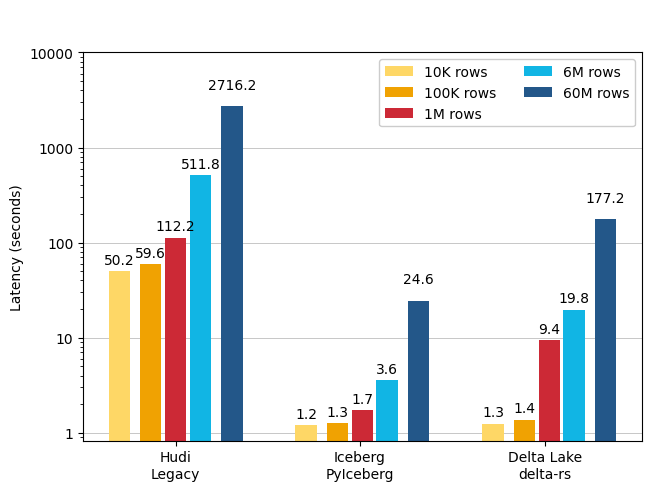
\includegraphics[width=\textwidth]{figures/5-results/hudi_iceberg_delta/write/write_time_1_core.png}
        \caption[Histogram of the write experiment - Latency - 1 CPU core]{Histogram in log-scale of the write experiment results expressed as latency. The experiment was performed with one \glstext{CPU} core.}
        \label{fig:res_write_time_HID}
    \end{minipage}
\end{figure}

\begin{figure}
    \centering
    \begin{minipage}[b]{\textwidth}
        \captionof{table}[Write experiments results expressed as throughput]{Write experiment results expressed as throughput. Experiments performed with multiple \glstext{CPU} cores are expressed as throughput percentage increase compared to the one \glstext{CPU} core experiment.}
        \label{tbl:res_write_throughput_cpu_perc_HID}
        \begin{tabular}{c r S[table-format=4.5] S[table-format=2.2] S[table-format=2.2] S[table-format=2.2]}
            \toprule
            Pipeline\Tstrut\Bstrut & {\thead{Number\\ of rows}} & {\thead{1 CPU core throughput \\ (k rows/second)}} & {\thead{2 CPU cores\\ (\% increase)}} & {\thead{4 CPU cores\\ (\% increase)}} & {\thead{8 CPU cores\\ (\% increase)}} \\
            \midrule
            \multirow{5}{4em}{Hudi\\Legacy}             &   10K   &      0.19905  &     -0.97  &     -2.02  &     -1.93  \\
                                                        &  100K   &      1.67909  &     -0.37  &      0.07  &     -1.21  \\
                                                        &    1M   &      8.91443  &      3.33  &      3.10  &      2.56  \\
                                                        &    6M   &     11.72221  &      8.13  &      6.20  &      7.54  \\
                                                        &   60M   &     22.08961  &     16.02  &     15.78  &     16.84  \\
            \midrule
            \multirow{5}{4em}{Iceberg\\PyIceberg}       &   10K   &      8.30521  &      0.75  &      0.74  &     -1.16  \\
                                                        &  100K   &     79.03658  &      5.47  &      0.84  &      1.33  \\
                                                        &    1M   &    582.17295  &     -0.22  &      5.28  &     -0.08  \\
                                                        &    6M   &   1677.62161  &      0.28  &      0.89  &      1.25  \\
                                                        &   60M   &   2438.04452  &      4.69  &      2.52  &      4.18  \\
            \midrule
            \multirow{5}{4em}{Delta Lake\\delta-rs}     &   10K   &      7.99435  &     -0.94  &      2.80  &     -8.00  \\
                                                        &  100K   &     73.09924  &      4.65  &      2.35  &      5.87  \\
                                                        &    1M   &    106.58358  &     10.12  &     11.45  &     13.11  \\
                                                        &    6M   &    303.77453  &     21.16  &     21.75  &     25.61  \\
                                                        &   60M   &    338.61080  &     32.08  &     42.83  &     45.37  \\
            \bottomrule
        \end{tabular}
    \end{minipage}
    \begin{minipage}[b]{\textwidth}
        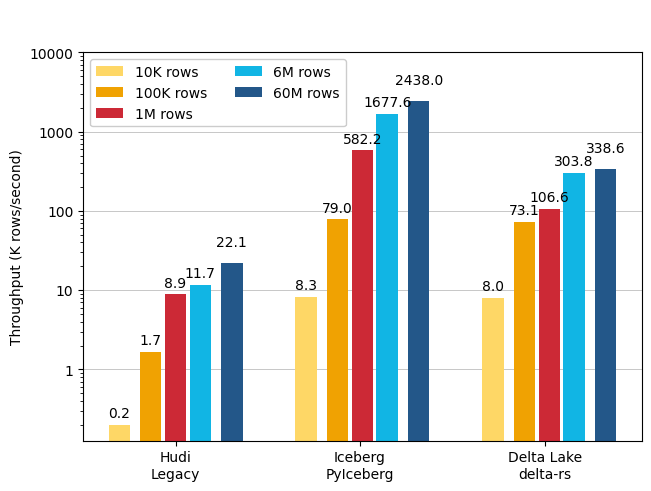
\includegraphics[width=\textwidth]{figures/5-results/hudi_iceberg_delta/write/write_throughput_1_core.png}
        \caption[Histogram of the write experiment - Throughput - 1 CPU core]{Histogram in log-scale of the write experiment results expressed as throughput. The experiment was performed with one \glstext{CPU} core.}
        \label{fig:res_write_throughput_HID}
    \end{minipage}
\end{figure}



Figures~\ref{fig:res_write_time_HID}--\ref{fig:res_write_throughput_HID}, and Tables~\ref{tbl:res_write_time_cpu_perc_HID}--\ref{tbl:res_write_throughput_cpu_perc_HID} report the results of the write experiments performed. The results are expressed in latency in Figure~\ref{fig:res_write_time_HID} and Table~\ref{tbl:res_write_time_cpu_perc_HID}, while are expressed in throughput in Figure~\ref{fig:res_write_throughput_HID} and Table~\ref{tbl:res_write_throughput_cpu_perc_HID}. The experiments were performed on the two systems defined in Section~\ref{subsec:experimental_design} and on the delta-rs based system defined in the related work \cite{manfrediReducingReadWrite2024}. The five tables of different sizes being written were defined in Section~\ref{subsec:experimental_data}.

Both histograms, i.e., Figures~\ref{fig:res_write_time_HID}--\ref{fig:res_write_throughput_HID}, report the results of the experiment performed with one \gls{CPU} core. Instead, Tables~\ref{tbl:res_write_time_cpu_perc_HID}--\ref{tbl:res_write_throughput_cpu_perc_HID} also present a calculated percentage of improvement (decrease in the case of latency, increase in the case of throughput) of the metric as the \gls{CPU} cores increase.


%%%%% WRITE RESULTS /// HUDI vs. ICEBERG %%%%%
\subsubsection*{Legacy pipeline vs. PyIceberg}




%%%%% WRITE RESULTS /// ICEBERG vs. DELTA LAKE %%%%%
\subsubsection*{PyIceberg vs. delta-rs}




%%%%% WRITE RESULTS /// PERFORMANCES WITH DIFFERENT CORE(S)
\subsubsection*{Change of performance as the \glsentryshort{CPU} cores increase}







%%%%%%%%%%%%%%%%%%%%%%%%%%%%%%%%%%%%%%%%%%%%%%%%%%%%%%%%%%%%%%%
%%%%%                  READ EXPERIMENTS                   %%%%%
%%%%%%%%%%%%%%%%%%%%%%%%%%%%%%%%%%%%%%%%%%%%%%%%%%%%%%%%%%%%%%%
\subsection{Read experiments}

\begin{figure}
    \centering
    \begin{minipage}[b]{\textwidth}
        \captionof{table}[Read experiments results expressed as latency]{Read experiment results expressed as latency. Experiments performed with multiple \glstext{CPU} cores are expressed as latency percentage decrease compared to the one \glstext{CPU} core experiment.}
        \label{tbl:res_read_time_cpu_perc_HID}
        \begin{tabular}{c r S[table-format=4.5] S[table-format=2.2] S[table-format=2.2] S[table-format=2.2]} 
            \toprule
            Pipeline\Tstrut\Bstrut & {\thead{Number\\ of rows}} & {\thead{1 CPU core latency \\ (seconds)}} & {\thead{2 CPU cores\\ (\% decrease)}} & {\thead{4 CPU cores\\ (\% decrease)}} & {\thead{8 CPU cores\\ (\% decrease)}} \\
            \midrule
            \multirow{5}{4em}{Hudi\\Legacy}             &   10K   &      0.63144  &      1.05  &     -0.76  &      0.65  \\
                                                        &  100K   &      2.65043  &     -0.49  &      0.40  &     -0.45  \\
                                                        &    1M   &      8.59296  &     -0.16  &     -1.76  &      2.80  \\
                                                        &    6M   &     33.52580  &      0.44  &      0.23  &      0.26  \\
                                                        &   60M   &     33.69031  &      0.18  &      0.09  &      1.63  \\
            \midrule
            \multirow{5}{4em}{Iceberg\\PyIceberg}       &   10K   &      0.01723  &     -6.36  &    -72.94  &      1.53  \\
                                                        &  100K   &      0.04687  &      7.89  &      8.62  &      8.95  \\
                                                        &    1M   &      0.43018  &     37.37  &     45.75  &     46.04  \\
                                                        &    6M   &      2.12331  &     38.96  &     52.50  &     58.34  \\
                                                        &   60M   &     21.81955  &     38.07  &     53.66  &     59.49  \\
            \midrule
            \multirow{5}{4em}{Delta Lake\\delta-rs}     &   10K   &      0.05345  &     22.90  &     18.50  &     19.29  \\
                                                        &  100K   &      0.05763  &      0.73  &      3.78  &      5.18  \\
                                                        &    1M   &      0.53878  &     56.62  &     64.81  &     67.69  \\
                                                        &    6M   &      1.94947  &     53.41  &     72.76  &     74.50  \\
                                                        &   60M   &     22.98186  &     50.35  &     75.72  &     87.19  \\
            \bottomrule
        \end{tabular}
    \end{minipage}
    \begin{minipage}[b]{\textwidth}
        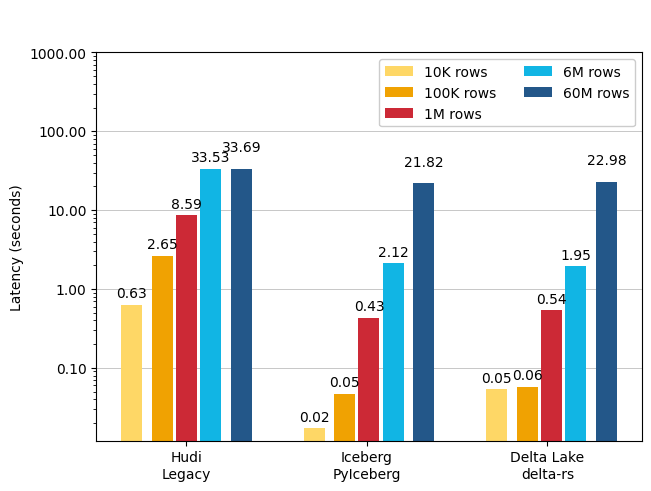
\includegraphics[width=\textwidth]{figures/5-results/hudi_iceberg_delta/read/read_time_1_core.png}
        \caption[Histogram of the read experiment - Latency - 1 CPU core]{Histogram in log-scale of the read experiment results expressed as latency. The experiment was performed with one \glstext{CPU} core.}
        \label{fig:res_read_time_HID}
    \end{minipage}
\end{figure}

\begin{figure}
    \centering
    \begin{minipage}[b]{\textwidth}
        \captionof{table}[Read experiments results expressed as throughput]{Read experiment results expressed as throughput. Experiments performed with multiple \glstext{CPU} cores are expressed as throughput percentage increase compared to the one \glstext{CPU} core experiment.}
        \label{tbl:res_read_throughput_cpu_perc_HID}
        \begin{tabular}{c r S[table-format=4.5] S[table-format=2.2] S[table-format=2.2] S[table-format=2.2]}
            \toprule
            Pipeline\Tstrut\Bstrut & {\thead{Number\\ of rows}} & {\thead{1 CPU core throughput \\ (k rows/second)}} & {\thead{2 CPU cores\\ (\% increase)}} & {\thead{4 CPU cores\\ (\% increase)}} & {\thead{8 CPU cores\\ (\% increase)}} \\
            \midrule
            \multirow{5}{4em}{Hudi\\Legacy}             &   10K   &     15.83673  &      1.06  &     -0.75  &      0.66  \\
                                                        &  100K   &     37.72979  &     -0.48  &      0.40  &     -0.45  \\
                                                        &    1M   &    116.37431  &     -0.16  &     -1.73  &      2.88  \\
                                                        &    6M   &    178.96662  &      0.44  &      0.23  &      0.26  \\
                                                        &   60M   &   1780.92764  &      0.18  &      0.09  &      1.65  \\
            \midrule
            \multirow{5}{4em}{Iceberg\\PyIceberg}       &   10K   &    580.48003  &     -5.98  &    -42.18  &      1.56  \\
                                                        &  100K   &   2133.40362  &      8.57  &      9.43  &      9.83  \\
                                                        &    1M   &   2324.62963  &     59.66  &     84.33  &     85.33  \\
                                                        &    6M   &   2825.77691  &     63.83  &    110.53  &    140.02  \\
                                                        &   60M   &   2749.82753  &     61.47  &    115.82  &    146.85  \\
            \midrule
            \multirow{5}{4em}{Delta Lake\\delta-rs}     &   10K   &    187.08171  &     29.70  &     22.69  &     23.89  \\
                                                        &  100K   &   1735.08031  &      0.74  &      3.93  &      5.47  \\
                                                        &    1M   &   1856.03325  &    130.51  &    184.19  &    209.48  \\
                                                        &    6M   &   3077.75801  &    114.64  &    267.09  &    292.19  \\
                                                        &   60M   &   2610.75520  &    101.42  &    311.87  &    680.55  \\
            \bottomrule
        \end{tabular}
    \end{minipage}
    \begin{minipage}[b]{\textwidth}
        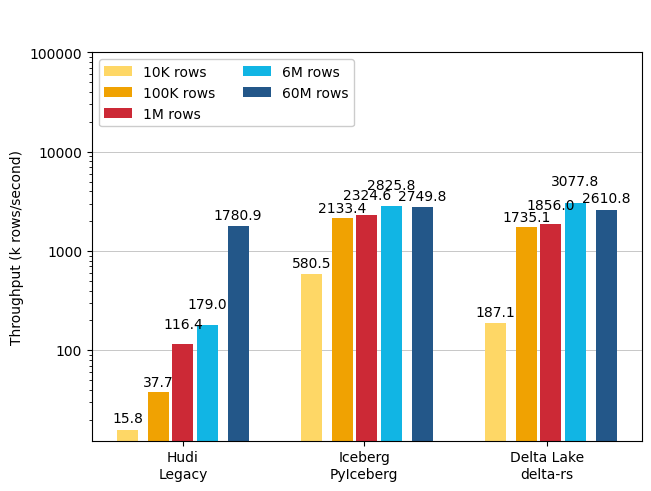
\includegraphics[width=\textwidth]{figures/5-results/hudi_iceberg_delta/read/read_throughput_1_core.png}
        \caption[Histogram of the read experiment - Throughput - 1 CPU core]{Histogram in log-scale of the read experiment results expressed as throughput. The experiment was performed with one \glstext{CPU} core.}
        \label{fig:res_read_throughput_HID}
    \end{minipage}
\end{figure}


Figures~\ref{fig:res_read_time_HID}--\ref{fig:res_read_throughput_HID}, and Tables~\ref{tbl:res_read_time_cpu_perc_HID}--\ref{tbl:res_read_throughput_cpu_perc_HID} report the results of the read experiments performed. The results are expressed in latency in Figure~\ref{fig:res_read_time_HID} and Table~\ref{tbl:res_read_time_cpu_perc_HID}, while are expressed in throughput in Figure~\ref{fig:res_read_throughput_HID} and Table~\ref{tbl:res_read_throughput_cpu_perc_HID}. The experiments were performed on the two systems defined in Section~\ref{subsec:experimental_design} and on the delta-rs based system defined in the related work \cite{manfrediReducingReadWrite2024}. The five tables of different sizes being read were defined in Section~\ref{subsec:experimental_data}.

Both histograms, i.e., Figures~\ref{fig:res_read_time_HID}--\ref{fig:res_read_throughput_HID}, report the results of the experiment performed with one \gls{CPU} core. Instead, Tables~\ref{tbl:res_read_time_cpu_perc_HID}--\ref{tbl:res_read_throughput_cpu_perc_HID} also present a calculated percentage of improvement (decrease in the case of latency, increase in the case of throughput) of the metric as the \gls{CPU} cores increase.



%%%%% WRITE RESULTS /// HUDI vs. ICEBERG %%%%%
\subsubsection*{Legacy pipeline vs. PyIceberg}




%%%%% WRITE RESULTS /// ICEBERG vs. DELTA LAKE %%%%%
\subsubsection*{PyIceberg vs. delta-rs}




%%%%% WRITE RESULTS /// PERFORMANCES WITH DIFFERENT CORE(S)
\subsubsection*{Change of performance as the \glsentryshort{CPU} cores increase}










%%%%%%%%%%%%%%%%%%%%%%%%%%%%%%%%%%%%%%%%%%%%%%%%%%%%%%%%%%%%%%%
%%%%%                  LEGACY BREAKDOWN                   %%%%%
%%%%%%%%%%%%%%%%%%%%%%%%%%%%%%%%%%%%%%%%%%%%%%%%%%%%%%%%%%%%%%%
\subsection{Legacy pipeline write latency breakdown}
\begin{figure}
    \centering
    \begin{minipage}[b]{\textwidth}
        \captionof{table}[Writes on legacy pipeline - Time breakdown]{Contributions to the write latency of the upload and materialization steps in the legacy pipeline. Experiments performed with multiple \glstext{CPU} cores are expressed as latency percentage decrease compared to the one \glstext{CPU} core experiment.}
        \label{tbl:hudi_virtualiz_breakdown_cpu_perc}
        \begin{tabular}{r S[table-format=4.2] S[table-format=4.2] S[table-format=2.2] S[table-format=2.2] S[table-format=2.2] S[table-format=2.2] S[table-format=2.2] S[table-format=2.2]} 
            \toprule
            \multirow{2}{*}{{\thead{Number\\ of rows}}} & \multicolumn{2}{c}{{\thead{1 CPU core\\ latency (seconds)}}} & \multicolumn{2}{c}{{\thead{2 CPU cores\\ (\% decrease)}}} & \multicolumn{2}{c}{{\thead{4 CPU cores\\ (\% decrease)}}} & \multicolumn{2}{c}{{\thead{8 CPU cores\\ (\% decrease)}}}\\
            & {upl.} & {mat.} & {upl.} & {mat.} & {upl.} & {mat.} & {upl.} & {mat.}\\
            \midrule
            10K &  2.50 & 47.73 & 4.50 & -1.28 & 4.53 & -2.46 & 4.65 & -2.32\\
            100K & 3.67 & 55.91 & 6.36 & -0.79 & 5.56 & -0.30 & 6.28 & -1.68\\
            1M   & 22.59 & 89.60 & 17.51 & -0.37 & 14.88 & 0.01 & 16.49 & -1.03\\
            6M   & 244.60 & 267.25 & 15.83 & -0.10 & 13.47 & -1.15 & 15.09 & -0.39\\
            60M &  2438.22 & 278.16 & 15.34 & 0.43 & 15.17 & 0.20 & 15.96 & 0.86\\
            \bottomrule
        \end{tabular}
    \end{minipage}
    \begin{minipage}[b]{\textwidth}
        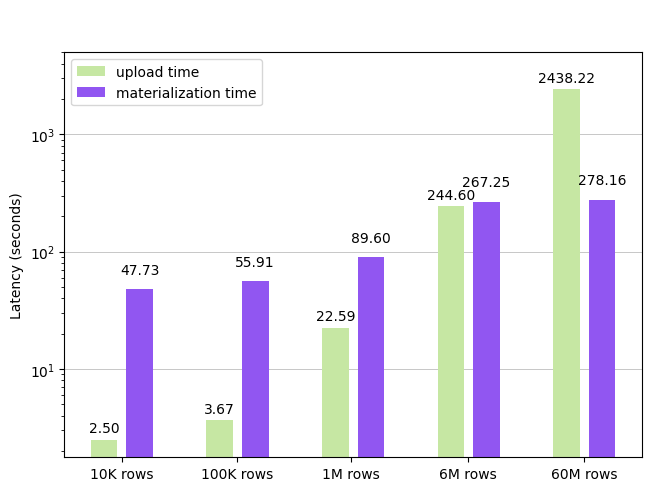
\includegraphics[width=\textwidth]{figures/5-results/hudi_iceberg_delta/hudi_virtualiz1_core.png}
        \caption[Histogram of the write on legacy pipeline - Time breakdown - 1 core]{Histogram in log-scale displaying the contributions to the write latency of the upload and materialization steps in the legacy pipeline. The experiment was performed with one \glstext{CPU} core.}
        \label{fig:hudi_virtualiz_breakdown}
    \end{minipage}
\end{figure}

Table \ref{tbl:hudi_virtualiz_breakdown_cpu_perc} and Figure \ref{fig:hudi_virtualiz_breakdown} show the write latency breakdown of the legacy pipeline into upload time and materialization time, the two different steps explained in Section \ref{subsec:back_sys_hudi_write}. The breakdown is proposed for all five tables defined in Section \ref{subsec:experimental_data}. Figure \ref{fig:hudi_virtualiz_breakdown} reports the data from the one \gls{CPU} core experiment. In contrast, Table \ref{tbl:hudi_virtualiz_breakdown_cpu_perc} reports both the one \gls{CPU} core experiment data and also a calculated percentage of improvement (decrease) of the latency as the \gls{CPU} cores increase.

Considering the upload time contribution to the write latency, this represents a small percentage (around 5\%) when writing smaller tables (10K and 100K) rows, while it grows following a similarly linear pattern in larger tables (100K, 6M, and 60M rows). This radically changes the proportion between the upload and materialized time contributions, making the upload time 90\% of the total write latency for the largest table (60M rows). Differently, the materialization time contribution makes up 95\% of the total write latency for the smallest table (10K rows), but then its absolute value does not increase by more than a significant figure even if the table size is increased by three significant figures.

Observing the results of experiments on multiple \gls{CPU} cores, the upload time benefits from a higher number of \gls{CPU} cores, especially with larger tables (15\% latency decrease compared to a 4\% with smaller tables), while the materialize time is not affected, having either small decreases in latency or small increases (both around 1-2\%).







%%%%%%%%%%%%%%%%%%%%%%%%%%%%%%%%%%%%%%%%%%%%%%%%%%%%%%%%%%%%%%%
%%%%%                   IN-MEMORY USAGE                   %%%%%
%%%%%%%%%%%%%%%%%%%%%%%%%%%%%%%%%%%%%%%%%%%%%%%%%%%%%%%%%%%%%%% 
\subsection{In-memory resources usage}
\label{subsec:resources_usage}

The resources of the experimental environment, defined in Section \ref{subsec:experimental_env}, were adjusted to match computational needs. The write operations were demanding on the available \gls{RAM} resources, requiring up to 24 GBs to operate with the larger tables (6M and 60M rows). Thus, on were allocated 32768 MBs of \gls{RAM}, to avoid slowing down operations.

\section{Related work results}
    \label{sec:related_work_results}
    \input{contents/5-results_and_analysis/2-related_results.tex}

\section{Results analysis and discussion}
    \label{sec:results_analysis_discussion}
    \input{contents/5-results_and_analysis/3-results_discussion.tex}

\cleardoublepage

\chapter{Conclusions and Future work}
    \label{ch:conclusions_and_future_work}
    \generalExpl{Add text to introduce the subsections of this chapter.}

\section{Conclusions}
\label{sec:conclusions}
\engExpl{Describe the conclusions (reflect on the whole introduction given in Chapter 1).}


  
\engExpl{Discuss the positive effects and the drawbacks.\\
Describe the evaluation of the results of the degree project.\\
Did you meet your goals?\\
What insights have you gained?\\
What suggestions can you give to others working in this area?\\
If you had it to do again, what would you have done differently?}

\section{Limitations}
\label{sec:limitations}
\engExpl{What did you find that limited your efforts? What are the limitations of your results?}


\section{Future work}
\label{sec:futureWork}
\engExpl{Describe valid future work that you or someone else could or should do.\\
Consider: What you have left undone? What are the next obvious things to be done? What hints can you give to the next person who is going to follow up on your work?}



Due to the breadth of the problem, only some of the initial goals have been
met. In these section we will focus on some of the remaining issues that
should be addressed in future work. ...

\subsection{What has been left undone?}
\label{what-has-been-left-undone}

The prototype does not address the third requirment, \ie a yearly unavailability of less than 3 minutes; this remains an open problem. ...

\subsubsection{Cost analysis}
\generalExpl{Example of a missing component}
The current prototype works, but the performance from a cost perspective makes this an impractical solution. Future work must reduce the cost of this solution; to do so, a cost analysis needs to first be done. ...

\subsubsection{Security}
\generalExpl{Example of a missing component}
A future research effort is needed to address the security holes that results from using a self-signed certificate. Page filling text mass. Page filling text mass. ...


\subsection{Next obvious things to be done}

In particular, the author of this thesis wishes to point out xxxxxx remains as a problem to be solved. Solving this problem is the next thing that should be done. ...

\section{Reflections}
\label{sec:reflections}
\generalExpl{What are the relevant economic, social, environmental, and ethical aspects of your work?}



One of the most important results is the reduction in the amount of
energy required to process each packet while at the same time reducing the
time required to process each packet.

The thesis contributes to the \gls{UN}\enspace\glspl{SDG} numbers 1 and 9 by
xxxx. 

%%%%%%%%%%%%%%%%%%%%%%%%%%%%%%%%%%%%%%%%%%%%%%%%%%%%%%%%%%%%%%%%%%%%%%%%%%%%%%%%%%%%%%%%
%%                                 REFERENCES
%%%%%%%%%%%%%%%%%%%%%%%%%%%%%%%%%%%%%%%%%%%%%%%%%%%%%%%%%%%%%%%%%%%%%%%%%%%%%%%%%%%%%%%%
%\noindent\rule{\textwidth}{0.4mm}
%\engExpl{In the references, let Zotero or other tool fill this in for you. I suggest an extended version of the IEEE style, to include URLs, DOIs, ISBNs, etc., to make it easier for your reader to find them. This will make life easier for your opponents and examiner. \\IEEE Editorial Style Manual: \url{https://www.ieee.org/content/dam/ieee-org/ieee/web/org/conferences/style_references_manual.pdf}}

\cleardoublepage

% Print the bibliography (and make it appear in the table of contents)
\renewcommand{\bibname}{References}

\ifbiblatex
    %\typeout{Biblatex current language is \currentlang}
    \printbibliography[heading=bibintoc]
\else
    \phantomsection  % make it include a hyperref - see https://tex.stackexchange.com/a/98995
    \addcontentsline{toc}{chapter}{References}
    \bibliography{references}
\fi

%%%%%%%%%%%%%%%%%%%%%%%%%%%%%%%%%%%%%%%%%%%%%%%%%%%%%%%%%%%%%%%%%%%%%%%%%%%%%%%%%%%%%%%%
%%                                 APPENDIX
%%%%%%%%%%%%%%%%%%%%%%%%%%%%%%%%%%%%%%%%%%%%%%%%%%%%%%%%%%%%%%%%%%%%%%%%%%%%%%%%%%%%%%%%
%% If you do not have an appendix, do not include the \textbackslash cleardoublepage command below; otherwise, the last page number in the metadata will be one too large.}
\cleardoublepage

\appendix
\renewcommand{\chaptermark}[1]{\markboth{Appendix \thechapter\relax:\thinspace\relax#1}{}}

\chapter{Supporting materials}
    \label{sec:supportingMaterial}
    This appendix contains the system architecture diagrams, for both the legacy system and the Apache Iceberg version.

\cleardoublepage

\chapter{Something Extra}
    This appendix contains the writing diagrams, showing the barplots and the schema with all the information the writing experiments performed on the different systems.

% Include an example of using nomenclature
\ifnomenclature
\cleardoublepage

\chapter{Main equations}
    \label{ch:NomenclatureExamples}
    This appendix contains the reading diagrams, showing the barplots and the schema with all the information the reading experiments performed on the different systems.


\cleardoublepage

%% The following label is necessary for computing the last page number of the body of the report to include in the "For DIVA" information
\label{pg:lastPageofMainmatter}

\cleardoublepage

%%%%%%%%%%%%%%%%%%%%%%%%%%%%%%%%%%%%%%%%%%%%%%%%%%%%%%%%%%%%%%%%%%%%%%%%%%%%%%%%%%%%%%%%
%%                                 FOR DIVA MATERIAL
%%%%%%%%%%%%%%%%%%%%%%%%%%%%%%%%%%%%%%%%%%%%%%%%%%%%%%%%%%%%%%%%%%%%%%%%%%%%%%%%%%%%%%%%
\clearpage\thispagestyle{empty}\mbox{} % empty page with backcover on the other side
\kthbackcover
\fancyhead{}  % Do not use header on this extra page or pages
\section*{€€€€ For DIVA €€€€}
\lstset{numbers=none} %% remove any list line numbering
\divainfo{pg:lastPageofPreface}{pg:lastPageofMainmatter}

% If there is an acronyms.tex file,
% add it to the end of the For DIVA information
% so that it can be used with the abstracts
% Note that the option "nolol" stops it from being listed in the List of Listings

% The following bit of ugliness is because of the problems PDFLaTeX has handling a non-breaking hyphen
% unless it is converted to UTF-8 encoding.
% If you do not use such characters in your acronyms, this could be simplified.
\ifxeorlua
\IfFileExists{lib/acronyms.tex}{
\section*{acronyms.tex}
\lstinputlisting[language={[LaTeX]TeX}, nolol, basicstyle=\ttfamily\color{black},
commentstyle=\color{black}, backgroundcolor=\color{white}]{lib/acronyms.tex}
}
{}
\else
\IfFileExists{lib/acronyms-for-pdflatex.tex}{
\section*{acronyms.tex}
\lstinputlisting[language={[LaTeX]TeX}, nolol, basicstyle=\ttfamily\color{black},
commentstyle=\color{black}, backgroundcolor=\color{white}]{lib/acronyms-for-pdflatex.tex}
}
{}
\fi

\end{document}
